\documentclass[11pt,a4paper,openany]{book}

% ---------- packages ----------
\usepackage[a4paper,margin=2.4cm]{geometry}
\usepackage[T1]{fontenc}
\usepackage[utf8]{inputenc}
\usepackage{mathpazo}
\usepackage{courier}
\usepackage{microtype}
\usepackage{amsmath,amssymb}
\usepackage{booktabs,array,tabularx}
\usepackage{enumitem}
\usepackage{xcolor}
\usepackage{tikz}
\usetikzlibrary{arrows.meta,positioning,calc,shapes.geometric,fit,backgrounds,decorations.pathreplacing}
\usepackage[most]{tcolorbox}
\usepackage{listings}
\usepackage{fancyhdr}
\usepackage{titlesec}
\usepackage[hidelinks]{hyperref}

\setlist{itemsep=2pt,topsep=4pt,parsep=0pt}
\renewcommand{\arraystretch}{1.18}
\setlength{\parskip}{4pt}
\setlength{\parindent}{0pt}

% ---------- headers ----------
\pagestyle{fancy}
\fancyhf{}
\fancyhead[LE]{\small\nouppercase{\leftmark}}
\fancyhead[RO]{\small\nouppercase{\rightmark}}
\fancyfoot[C]{\thepage}
\renewcommand{\headrulewidth}{0.3pt}
\titleformat{\chapter}[display]{\normalfont\huge\bfseries\color{blue!40!black}}{\chaptertitlename\ \thechapter}{10pt}{\Huge}
\titlespacing*{\chapter}{0pt}{-10pt}{22pt}

% ---------- colours / boxes ----------
\definecolor{defblue}{RGB}{30,80,160}
\definecolor{intgreen}{RGB}{30,120,70}
\definecolor{warnred}{RGB}{170,40,40}
\definecolor{exorange}{RGB}{200,110,20}
\definecolor{keypurple}{RGB}{110,50,150}

\tcbset{nbox/.style={enhanced,breakable,arc=2pt,boxrule=0.6pt,left=7pt,right=7pt,top=4pt,bottom=4pt,
  fonttitle=\bfseries\small,before skip=9pt,after skip=9pt}}
\newtcolorbox{definition}[1]{nbox,colback=defblue!5,colframe=defblue,title={Definition: #1}}
\newtcolorbox{intuition}{nbox,colback=intgreen!6,colframe=intgreen,title={In plain words}}
\newtcolorbox{pitfall}{nbox,colback=warnred!5,colframe=warnred,title={Watch out}}
\newtcolorbox{workedex}[1]{nbox,colback=exorange!6,colframe=exorange,title={Worked example: #1}}
\newtcolorbox{keyidea}{nbox,colback=keypurple!6,colframe=keypurple,title={Key idea}}

\newtcolorbox{outofsyllabus}{nbox,colback=gray!10,colframe=black!70,title={OUT OF SYLLABUS}}
\newcommand{\oos}{\noindent{\small\textcolor{red!60!black}{\textsc{Out of syllabus (not on the slides)}}}\par\smallskip}
\newcommand{\slides}[1]{\noindent{\small\textcolor{teal!70!black}{\textsc{Matches slides #1}}}\par\smallskip}
\newcommand{\term}[1]{\textbf{\textit{#1}}}
\newcommand{\cl}[1]{\texttt{#1}}

% ---------- listings ----------
\lstset{language=C,basicstyle=\ttfamily\small,keywordstyle=\color{blue!60!black}\bfseries,
  commentstyle=\color{green!40!black}\itshape,numbers=left,numberstyle=\tiny\color{gray},
  frame=single,framerule=0.3pt,breaklines=true,columns=fullflexible,
  xleftmargin=1.6em,framexleftmargin=1.6em,aboveskip=8pt,belowskip=8pt}

% ---------- tikz styles ----------
\tikzset{
  >=Stealth,
  pe/.style={draw,rounded corners=2pt,fill=blue!12,minimum width=9mm,minimum height=6.5mm,font=\small},
  mm/.style={draw,fill=orange!18,minimum width=9mm,minimum height=6.5mm,font=\small},
  ca/.style={draw,fill=green!15,minimum width=9mm,minimum height=4.5mm,font=\scriptsize},
  swt/.style={draw,fill=gray!22,minimum size=5mm,font=\scriptsize},
  busbar/.style={draw,fill=gray!18,minimum height=5mm,font=\scriptsize},
  lnk/.style={thick},
  dn/.style={circle,draw,fill=blue!12,minimum size=6mm,inner sep=0pt,font=\scriptsize},
}

\title{\textbf{Parallel and Many-core Architecture}\\[4pt]\Large Study notes to read alongside the slides\\[2pt]\large DS221: Introduction to Scalable Systems}
\author{}
\date{\today}

\begin{document}
\frontmatter
\maketitle

\chapter*{Preface}
\addcontentsline{toc}{chapter}{Preface}

These notes accompany the slide decks \emph{Parallel Architecture} and \emph{Many-core Architectures} used in DS221. The slides are
short: each bullet stands for a few minutes of explanation in class. The notes are meant to
supply that explanation, so that a student who missed the lectures, or who has never studied
computer systems before, can follow every step.

\subsection*{How to use the notes}
\begin{itemize}
  \item Each section starts with a line such as \textsc{Matches slides 5--7}. Read the slides
        first, then the section, then try the exercises at the end of the chapter.
  \item The order of material follows the slides: why parallel hardware exists (Chapter~1),
        how parallel machines are classified (Chapter~2), caches and cache coherence
        (Chapter~3), and interconnection networks (Chapter~4). Chapter~5 is a summary, a
        formula sheet and a glossary. The second part is about many-core processors: why GPUs exist (Chapter~6), the
        NVIDIA A100 chip (Chapter~7) and the GPU memory hierarchy (Chapter~8), with its own summary in Chapter~9. Chapter~10 goes deeper into the A100 than the slides do and is marked as \textbf{out of syllabus} throughout.
  \item Solutions to all exercises are in Appendix~A. Try them before looking.
\end{itemize}

\subsection*{What is assumed}
(For Chapters 6--9 the same assumptions hold; GPU numbers come from the NVIDIA A100 whitepaper, which the course lists as reading.)\par\smallskip
You should know what a cache is and what a cache hit and miss are, how a memory address is split
into tag, index and offset, and why locality matters. These are covered in Chapter~1 of Nihar
Shah's notes (\emph{Notes on Parallel Computing}), which the notes below build on. One idea that
is usually taught alongside caches but is \emph{not} covered there, the \emph{write policy}
(write-through versus write-back and the dirty bit), is explained here in
Section~\ref{sec:writepolicy} because cache coherence depends on it.

\subsection*{The boxes}
\begin{definition}{a term}
Blue boxes define a term precisely. These are the words the slides and exams use.
\end{definition}
\begin{intuition}
Green boxes restate an idea informally, often with an analogy.
\end{intuition}
\begin{workedex}{a calculation}
Orange boxes work through numbers or a trace step by step.
\end{workedex}
\begin{pitfall}
Red boxes mark common misconceptions and easy mistakes.
\end{pitfall}
\begin{keyidea}
Purple boxes hold the one thing to remember from a section.
\end{keyidea}

\subsection*{A note on sources}
The structure follows the slides. Where the notes go beyond the slides (for example, the cost
model for messages, or the counting argument for Omega networks) this is said explicitly. Standard
references are listed in Chapter~5: Grama, Gupta, Karypis and Kumar for networks, and Culler and
Singh for caches and coherence. All text and figures here are original.

\tableofcontents

\mainmatter
\chapter{Why Parallel Computers?}
\label{ch:why}

\slides{2}

Every slide deck on parallel computing starts by saying that processors stopped getting faster.
That sounds odd: a laptop today is certainly faster than one from ten years ago. This chapter
explains what stopped, what did not, and why the industry's answer was to put \emph{many} processors on a chip
instead of one faster one.

\section{The free lunch is over}

For roughly thirty years, a programmer could write a program once and expect it to run faster on
every new generation of computer, with no changes at all. Two trends made this possible:

\begin{itemize}
  \item \textbf{More transistors.} A transistor is the tiny electronic switch that all digital
        circuits are built from. \term{Moore's law} is the observation that the number of
        transistors that fit on a chip doubles roughly every two years. This is still
        approximately true.
  \item \textbf{Higher clock frequency.} A processor does its work in steps called
        \emph{cycles}, paced by a clock. A $3$~GHz clock ticks three billion times per second.
        If you can raise the clock frequency, every instruction finishes sooner and every program speeds up.
\end{itemize}

The second trend is the one that ended. Clock frequencies climbed from a few MHz in the early
1980s to about $3$--$4$~GHz in the mid-2000s and then stopped, and they have stayed there. The
slide says it briefly: \emph{``CPU speeds have saturated''}. There are two main reasons.

\subsection{The power wall}

A chip turns almost all the electrical power it uses into heat. The \emph{dynamic} power of a
chip (the power spent switching transistors) is approximately
\begin{equation}
  P \;\approx\; \alpha\, C\, V^{2} f ,
  \label{eq:power}
\end{equation}
where $f$ is the clock frequency, $V$ the supply voltage, $C$ the total capacitance being
switched (roughly: how much circuitry there is), and $\alpha$ the fraction of the circuit that
switches in each cycle.

The catch is that $V$ cannot be chosen freely. A faster clock needs transistors to switch faster, which needs a
higher voltage. To a first approximation $V$ grows in proportion to $f$, so
\[
  P \;\propto\; f^{3}.
\]
Doubling the frequency would need about eight times the power, and that power has to leave the
chip as heat through an area the size of a postage stamp. Air cooling can remove on the order of
100~watts from a chip; beyond that you need exotic cooling that is too expensive for ordinary computers.
So frequency stopped rising.

\begin{workedex}{two slow cores beat one fast core}
Suppose one core runs at frequency $f$ and voltage $V$ and uses power $P_0$. Now run a core at
$0.8f$. Under the simplification $V \propto f$ it needs only $0.8V$, so its power is
\[
  P = 0.8 \times (0.8)^2 \, P_0 = 0.512\,P_0 .
\]
Two such cores together use $2\times 0.512\,P_0 \approx 1.02\,P_0$, essentially the same power as the
original single core, but if the work can be shared perfectly they deliver $2\times 0.8 = 1.6$
times the throughput. Making a chip with more, slower cores is therefore a far better use of a fixed power budget than
making a single core faster.
\end{workedex}

This is the central reason that parallel hardware became mandatory. The example hides an
important condition, though: ``\emph{if the work can be shared perfectly}''. The hardware
now offers parallelism; the software has to use it.

\subsection{The memory wall}

The second reason is that processors became much faster than main memory (DRAM). Two different
quantities matter here:

\begin{definition}{latency and bandwidth}
\textbf{Latency} is the time one request takes from start to finish, for example the time
between a core asking for a value and receiving it. \textbf{Bandwidth} is the amount of data
moved per unit time, for example gigabytes per second.
\end{definition}

\begin{intuition}
Think of a road. Latency is how long one car takes to drive from A to B. Bandwidth is how many cars
per hour the road can carry. A road can have low latency and low bandwidth (one fast lane) or the other way round
(a wide, slow motorway).
\end{intuition}

A main-memory access takes on the order of $100$~ns. At $3$~GHz that is hundreds of cycles during
which the core could have executed many instructions. Caches (your Chapter~1) hide much of this
latency by keeping recently used data close to the core. But caches do not help a program that
streams through a huge array once, and the memory \emph{bandwidth} of a chip is also finite and is
shared by all of its cores.

\begin{pitfall}
More cores do not automatically fix the memory wall. They bring more caches and more
opportunities to overlap computation with data movement, but they also compete for the same memory
bandwidth. This is one reason real machines have several memory channels and, as we will see in Chapter~2,
why large machines distribute their memory among processors (NUMA).
\end{pitfall}

\subsection{A third limit: instruction-level parallelism}

Inside a single core, hardware already runs several instructions at once when they do not depend on each other.
This is \term{instruction-level parallelism} (ILP): pipelining, several execution units, out-of-order
execution. It is invisible to the programmer. But finding independent instructions within one stream of ordinary code is
hard, and each extra bit of ILP costs a lot of hardware, so there are rapidly diminishing returns after a few instructions per cycle.
The remaining place to find parallelism is \emph{between} streams of instructions, which is
what multiple cores and multiple machines provide.

\section{Reasons to use parallel computing}

The slide lists four motivations. Each is worth stating in full.

\begin{enumerate}
  \item \textbf{Faster execution.} A computation that takes days or months on one core might
        take hours or seconds on many. Climate modelling and bioinformatics are the slide's examples:
        a weather forecast that arrives after the weather is useless.
  \item \textbf{Large amounts of data.} Some data sets do not fit in the memory of one machine,
        or take too long to scan with one processor. If a data set is 10~TB and one machine has 64~GB
        of RAM, the data must be spread over many machines and processed in parallel.
  \item \textbf{Natural parallelism.} Many problems are made of many similar, nearly independent parts.
        In a climate model the atmosphere is divided into a grid of cells, and the same update rule is applied to each
        cell. Writing this as a serial loop \emph{hides} parallelism that was in the problem all along.
  \item \textbf{Architecture trends.} The power and memory walls above: since a single core cannot be
        made much faster, the only way to use more transistors is to build more cores.
\end{enumerate}

There are two different goals hidden in these. One is to solve the \emph{same problem faster}; the
other is to solve a \emph{bigger problem in the same time}. Later slides give them precise names
(strong and weak scaling).

\section{Vocabulary used throughout}

Parallel computing uses a lot of words that sound alike. Fix the meanings now.

\begin{center}
\begin{tabularx}{\linewidth}{@{}l X@{}}
\toprule
\textbf{Term} & \textbf{Meaning in these notes}\\
\midrule
Core & One unit that executes one stream of instructions (possibly two when hyper-threading is used).\\
Processor / socket / chip & A package containing one or several cores. Slides often say ``processor''
  loosely to mean any processing element, so $P_1, P_2,\ldots$ may be cores or whole machines.\\
Node & One complete computer (``one box''): one or more sockets plus memory, disk and a network card.\\
Cluster & Many nodes connected by a network and used together. A supercomputer is in practice a very large cluster
  with a very fast network.\\
Process & A running program with its \emph{own} private address space.\\
Thread & An independent flow of execution \emph{inside} a process; all threads of a process share its memory.\\
Parallel & Several things really executing at the same instant (needs several cores).\\
Concurrent & Several things in progress, possibly interleaved on one core. All parallel programs are
  concurrent; not all concurrent programs are parallel.\\
\bottomrule
\end{tabularx}
\end{center}

\section{Not everything can be parallelised}

The slides remark that parallelism is ``more natural for certain kinds of problems''. The flip side is that
some work is inherently sequential: step~2 needs the result of step~1. If a fraction $s$ of a
program's running time is inherently serial, then no matter how many processors you use, the
speedup can never exceed $1/s$. A program that is $10\%$ serial can never run more than $10\times$
faster. The proper treatment (Amdahl's law) comes with the parallelisation-principles slides; keep this
number in mind.

\begin{keyidea}
Physics (power and memory limits) forced hardware designers to provide parallelism instead of
speed. Programmers now have to expose that parallelism in their programs. The rest of this part of the
course asks: what does parallel hardware look like, how do its parts talk to each other, and what does
that mean for performance?
\end{keyidea}

\section*{Exercises}
\addcontentsline{toc}{section}{Exercises}
\begin{enumerate}[label=\textbf{\thechapter.\arabic*},leftmargin=*]
  \item Using $P\propto f^3$, by what factor does the dynamic power of a core change if its clock frequency
        is raised by $25\%$?
  \item A core at frequency $f$ uses power $P_0$. Using the same simplified model, how much
        power do eight cores at $0.5f$ use in total, and what is their throughput relative to one core at $f$
        (assuming perfectly parallel work)?
  \item A program must read 12.8~GB from memory exactly once, and the memory system delivers
        25.6~GB/s. What is the shortest possible running time, regardless of how many cores are used or how
        low the latency is?
  \item A program is 5\% inherently serial. What is the largest possible speedup, and what speedup
        do 16 cores give? (Use $S(n)=1/(s+(1-s)/n)$.)
  \item Explain the difference between latency and bandwidth using an example other than a road.
\end{enumerate}
\chapter{Classifying Parallel Machines}
\label{ch:classify}

There are many kinds of parallel computer, and the slides give two ways of sorting them. The first looks
at \emph{what is executed in parallel} (Flynn's classification). The second looks at \emph{how memory is organised}
(shared versus distributed). Both are needed to understand the rest of the course.

\section{Flynn's classification}
\slides{3--4}

Michael Flynn proposed in the 1960s that computers can be classified by counting two kinds of
\emph{streams}:

\begin{definition}{instruction stream and data stream}
The \textbf{instruction stream} is the sequence of instructions a processor fetches and executes.
The \textbf{data stream} is the sequence of data items those instructions operate on.
\end{definition}

Each stream can be single or multiple, which gives four combinations:

\begin{center}
\begin{tabular}{@{}l|c|c@{}}
 & \textbf{Single data} & \textbf{Multiple data}\\ \hline
\textbf{Single instruction} & SISD & SIMD\\ \hline
\textbf{Multiple instruction} & MISD & MIMD\\
\end{tabular}
\end{center}

\subsection{SISD: the ordinary serial computer}

One instruction is executed at a time, on one piece of data at a time. This is the classical model
of a computer, a single core running a single thread. (Inside the core, ILP overlaps several
instructions, but the \emph{programming model} is still one stream.)

\subsection{SIMD: one instruction, many data items}

In a SIMD machine a single control unit sends the \emph{same} instruction to many processing elements,
and each element applies it to \emph{its own} data. All elements work in \term{lock-step}: at every moment they are
all executing the same instruction.

The slide's example is the element-wise product $C(i)=A(i)\times B(i)$ for $i=1,\dots,n$.
Give each processing element $P_i$ one index $i$. Every element then performs the same four steps, at the
same time, on different data:

\begin{center}
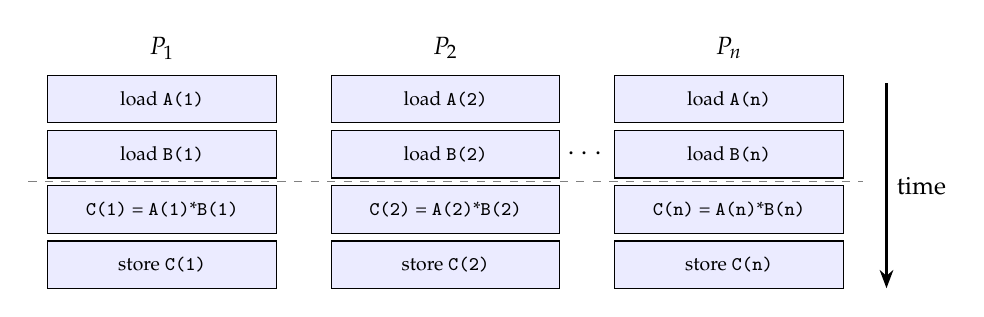
\begin{tikzpicture}[bx/.style={draw,minimum width=2.9cm,minimum height=6mm,font=\scriptsize,fill=blue!8}]
  \foreach \x/\lab/\i in {0/{$P_1$}/1, 3.6/{$P_2$}/2, 7.2/{$P_n$}/n} {
     \node[bx] at (\x,0)    {load \cl{A(\i)}};
     \node[bx] at (\x,-0.7) {load \cl{B(\i)}};
     \node[bx] at (\x,-1.4) {\cl{C(\i)} = \cl{A(\i)}*\cl{B(\i)}};
     \node[bx] at (\x,-2.1) {store \cl{C(\i)}};
     \node[font=\small\bfseries] at (\x,0.65) {\lab};
  }
  \node at (5.4,-0.7) {$\cdots$};
  \draw[->,thick] (9.2,0.2) -- (9.2,-2.4) node[midway,right,font=\small]{time};
  \draw[dashed,gray] (-1.7,-1.05) -- (8.9,-1.05);
\end{tikzpicture}
\end{center}

The dashed line illustrates lock-step: at the instant it marks, every element is in the same step.

\textbf{Where SIMD appears in real hardware.}
\begin{itemize}
  \item \emph{Vector processors} (Cray-90, Cray YMP in the slide): one instruction operates on a whole
        \emph{vector register} of numbers.
  \item \emph{Processor arrays} (the Connection Machine CM-2): thousands of simple processing
        elements under one control unit.
  \item \emph{SIMD instructions in today's CPUs}: SSE and AVX instructions process several numbers per
        instruction. An AVX-512 register is 512 bits wide and holds eight 64-bit doubles, so one instruction
        performs eight additions. Compilers use these automatically when they can prove the loop iterations
        are independent. This is the topic of ``vectorisation'' in your Chapter~1, section~1.5.
  \item \emph{GPUs}: threads are executed in groups that run the same instruction together. This is covered in the many-core
        slides.
\end{itemize}

\begin{pitfall}
\textbf{Branches hurt SIMD.} Suppose a loop body is \cl{if (x[i] > 0) y[i] = f(x[i]); else y[i] = g(x[i]);}
and eight lanes process eight values at once. The lanes cannot go different ways, since there is only one instruction stream. The
hardware first executes the \cl{f} path with the lanes where the condition is false switched off (``masked''), then the \cl{g}
path with the other lanes masked. Both paths are executed, and the cost is the \emph{sum}. SIMD works best on regular,
branch-free code.
\end{pitfall}

\subsection{MISD: multiple instructions, one data stream}

Several processing elements execute \emph{different} instructions on the \emph{same} data. The slide
simply says ``not popular''. The few uses are in fault-tolerant systems, where several units compute the same
result in different ways and a vote decides the answer, so that a single faulty unit is outvoted. Some authors count
systolic arrays here; others do not. For this course MISD is a box in the table and little else.

\subsection{MIMD: multiple instructions, multiple data}

Every processing element has its own instruction stream and its own data, and they run
\emph{independently and asynchronously}. At the same moment, one may be multiplying vectors while another
sorts a list and a third waits for input:

\begin{center}
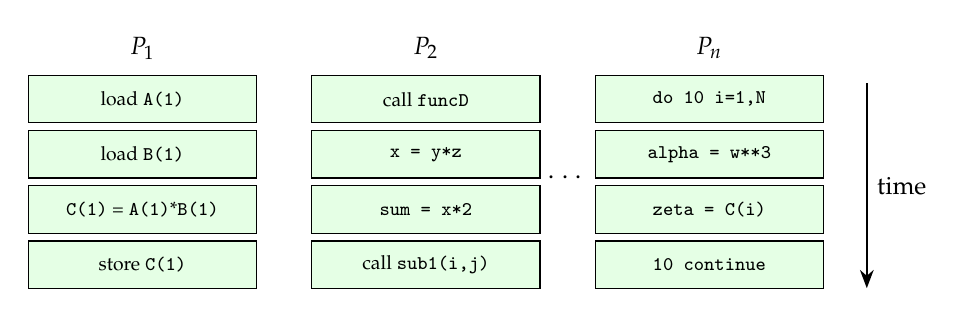
\begin{tikzpicture}[bx/.style={draw,minimum width=2.9cm,minimum height=6mm,font=\scriptsize,fill=green!10}]
  \node[font=\small\bfseries] at (0,0.65)   {$P_1$};
  \node[font=\small\bfseries] at (3.6,0.65) {$P_2$};
  \node[font=\small\bfseries] at (7.2,0.65) {$P_n$};
  \node[bx] at (0,0)    {load \cl{A(1)}};
  \node[bx] at (0,-0.7) {load \cl{B(1)}};
  \node[bx] at (0,-1.4) {\cl{C(1)} = \cl{A(1)}*\cl{B(1)}};
  \node[bx] at (0,-2.1) {store \cl{C(1)}};
  \node[bx] at (3.6,0)    {call \cl{funcD}};
  \node[bx] at (3.6,-0.7) {\cl{x = y*z}};
  \node[bx] at (3.6,-1.4) {\cl{sum = x*2}};
  \node[bx] at (3.6,-2.1) {call \cl{sub1(i,j)}};
  \node[bx] at (7.2,0)    {\cl{do 10 i=1,N}};
  \node[bx] at (7.2,-0.7) {\cl{alpha = w**3}};
  \node[bx] at (7.2,-1.4) {\cl{zeta = C(i)}};
  \node[bx] at (7.2,-2.1) {\cl{10 continue}};
  \node at (5.4,-1.0) {$\cdots$};
  \draw[->,thick] (9.2,0.2) -- (9.2,-2.4) node[midway,right,font=\small]{time};
\end{tikzpicture}
\end{center}

MIMD is the most general and by far the most common model: multicore laptops, clusters,
supercomputers (the slide's list: IBM SP, ``most other supercomputers, clusters, computational grids'').

\begin{intuition}
SIMD is a drill sergeant: every soldier does the same movement at the same moment. MIMD is a team of
workers, each with their own task list. SIMD is cheaper per unit of work when the task is regular; MIMD is
flexible enough for anything.
\end{intuition}

\paragraph{SPMD, a programming style (not a Flynn class).}
Most MPI programs are written as \term{SPMD}: Single Program, Multiple Data. Every process runs
\emph{the same program text}, but each uses its own identity (its \emph{rank}) to decide which part of the data to work on.
Because the processes run at their own pace and may take different branches, the hardware executing an SPMD program is MIMD,
\emph{not} SIMD. Do not confuse the two.

\begin{pitfall}
``A multicore CPU is SIMD'' is wrong. The \emph{cores} are independent, so the chip is MIMD. But \emph{inside each
core} there are SIMD units. Real machines combine both: MIMD across cores and SIMD within each core.
\end{pitfall}

\section{Classification by memory organisation}
\slides{5--7}

The second classification asks: when two processors want to exchange data, \emph{how do they do it}?
The answer depends on how memory is organised, and this choice shapes how parallel programs are written
more than any other. To state it precisely we first need the idea of an address space.

\subsection{Background: addresses and address spaces}

Memory can be pictured as a very long row of numbered boxes, one per byte. The box number is the
\term{address}. A pointer in C is just such a number. There are two kinds:
\begin{itemize}
  \item A \term{virtual address} is the number the \emph{program} uses. Each process sees its own private virtual
        address space, starting from zero. The operating system and hardware translate it.
  \item A \term{physical address} identifies an actual location in the DRAM chips.
\end{itemize}
Two different processes may both use the virtual address \cl{0x7FFF5FBFFD98} and refer to completely different
data, because their translations differ. This shows that the number alone means nothing until you also know \emph{whose} address space it
belongs to.

\begin{definition}{shared physical address space}
All processors address the same collection of memory locations: a given physical address refers to the \emph{same}
storage location no matter which processor uses it. If $P_1$ writes to that address, $P_2$
reading it sees the new value.
\end{definition}

\subsection{Shared-memory machines}

\begin{center}
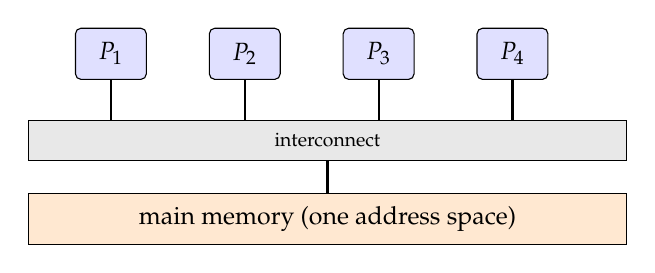
\begin{tikzpicture}
  \foreach \i in {1,2,3,4} { \node[pe] (p\i) at (\i*1.7,2.1) {$P_\i$}; }
  \node[busbar,minimum width=7.6cm] (ic) at (3.4*1.25+0.2,1.0) {interconnect};
  \node[mm,minimum width=7.6cm] (m) at (3.4*1.25+0.2,0) {main memory (one address space)};
  \foreach \i in {1,2,3,4} { \draw[lnk] (p\i) -- (p\i |- ic.north); }
  \draw[lnk] (ic) -- (m);
\end{tikzpicture}
\end{center}

In a \term{shared-memory machine} all processors are connected to a common memory. Processors
communicate \emph{implicitly}: one writes a variable, another reads it, with ordinary loads and
stores. There are no explicit ``send'' operations. Programming is comparatively easy because data does not
have to be moved by hand, and the usual interface is \emph{threads} (OpenMP, pthreads). But it brings its own problems:

\begin{itemize}
  \item \textbf{Race conditions.} If two threads read and write the same location with no coordination, the result depends on
        timing. Take \cl{x = x + 1} executed by two threads, with \cl{x} initially $0$. The statement is really three steps
        (read \cl{x}, add one, write back):

  \begin{center}
  \begin{tabular}{@{}lll@{}}
  \toprule
  Step & Thread A & Thread B\\
  \midrule
  1 & read $x$ (gets $0$) & \\
  2 &  & read $x$ (gets $0$)\\
  3 & write $x=1$ & \\
  4 &  & write $x=1$\\
  \bottomrule
  \end{tabular}
  \end{center}
  Two increments were executed but $x=1$: one update was lost. Preventing this needs \emph{synchronisation}
  (locks, atomic operations), which later slides cover.
  \item \textbf{Cache coherence.} Each processor has its own cache holding \emph{copies} of memory.
        Keeping those copies consistent is a hardware problem (Chapter~3).
  \item \textbf{Contention.} Many processors using the same memory at once compete for its bandwidth.
\end{itemize}

\subsection{UMA and NUMA}

Shared-memory machines come in two kinds, depending on whether all memory is equally far from all processors.

\begin{center}
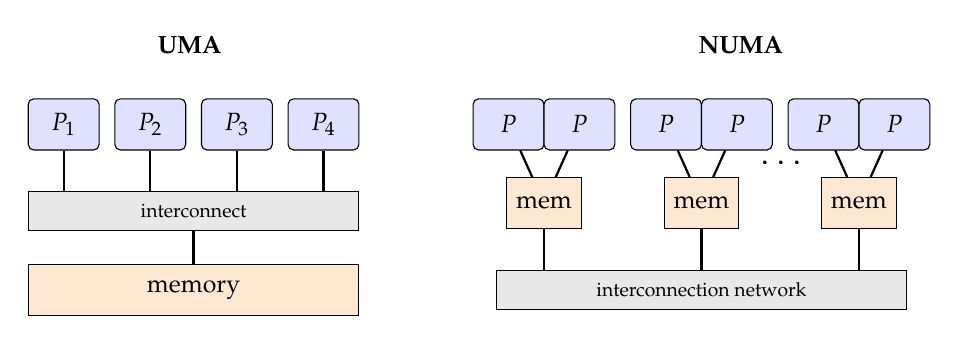
\begin{tikzpicture}[xscale=1.0]
  % UMA
  \node[font=\small\bfseries] at (1.6,3.5) {UMA};
  \node[pe] (a1) at (0,2.5) {$P_1$}; \node[pe] (a2) at (1.1,2.5) {$P_2$};
  \node[pe] (a3) at (2.2,2.5) {$P_3$}; \node[pe] (a4) at (3.3,2.5) {$P_4$};
  \node[busbar,minimum width=4.2cm] (ia) at (1.65,1.4) {interconnect};
  \node[mm,minimum width=4.2cm] (ma) at (1.65,0.4) {memory};
  \foreach \i in {1,2,3,4} \draw[lnk] (a\i) -- (a\i |- ia.north);
  \draw[lnk] (ia) -- (ma);
  % NUMA
  \node[font=\small\bfseries] at (8.6,3.5) {NUMA};
  \foreach \k/\x in {1/6.1,2/8.1,3/10.1} {
     \node[pe] (np\k) at (\x-0.45,2.5) {$P$}; \node[pe] (nq\k) at (\x+0.45,2.5) {$P$};
     \node[mm] (nm\k) at (\x,1.5) {mem};
     \draw[lnk] (np\k) -- (nm\k); \draw[lnk] (nq\k) -- (nm\k);
  }
  \node[busbar,minimum width=5.2cm] (ib) at (8.1,0.4) {interconnection network};
  \foreach \k in {1,2,3} \draw[lnk] (nm\k) -- (nm\k |- ib.north);
  \node at (9.15,2.0) {\large$\cdots$};
\end{tikzpicture}
\end{center}

\begin{definition}{UMA (Uniform Memory Access)}
Every processor needs the same time to access every memory location. These machines are also called
\emph{symmetric multiprocessors} (SMP). Data placement does not matter for performance.
\end{definition}

\begin{definition}{NUMA (Non-Uniform Memory Access)}
Memory is split into pieces attached to particular processors (or groups of them). A processor reaches
its \emph{local} memory quickly and \emph{remote} memory (attached to another processor) more slowly, but it is
\emph{still one shared address space}: the hardware carries out a remote load or store transparently. With coherent caches
this is called cc-NUMA.
\end{definition}

\textbf{Why does NUMA exist?} A single memory module, or a single bus to it, can only deliver a limited
bandwidth. If dozens of processors share it, it saturates. Attaching a piece of memory to each processor (or small group) multiplies the
total bandwidth with the number of processors, at the price of uneven access times. The machines named in
the slide (HP Exemplar, SGI Origin, Sequent NUMA-Q) are older examples. Today any multi-socket server is
NUMA: each socket has its own memory controller and DRAM, so a two-socket machine has two NUMA nodes. Remote
accesses typically cost noticeably more than local ones, often $1.5$ to $3$ times as much.

\begin{pitfall}
\textbf{NUMA is not distributed memory.} In NUMA a processor \emph{can} load from any memory in the machine
directly. In a distributed-memory machine (below) it cannot: the other node's memory is not in its address space.
\end{pitfall}

\textbf{What NUMA means for programmers.} The operating system normally places a memory page on the node of the thread that
\emph{first touches} it (the ``first-touch'' policy). If one thread initialises a huge array alone and then many threads on both sockets
process it, half the accesses become remote. Good NUMA code initialises data in parallel with the same distribution that
will later be used to compute on it. This is a performance issue only: the program is correct either way.

\subsection{Distributed-memory (message-passing) machines}

\begin{center}
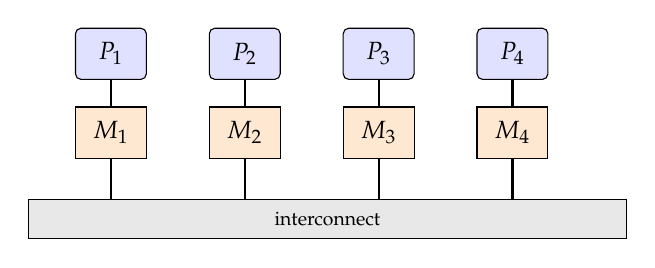
\begin{tikzpicture}
  \foreach \i in {1,2,3,4} {
    \node[pe] (p\i) at (\i*1.7,2.1) {$P_\i$};
    \node[mm] (m\i) at (\i*1.7,1.1) {$M_\i$};
    \draw[lnk] (p\i) -- (m\i);
  }
  \node[busbar,minimum width=7.6cm] (ic) at (3.4*1.25+0.2,0) {interconnect};
  \foreach \i in {1,2,3,4} \draw[lnk] (m\i) -- (m\i |- ic.north);
\end{tikzpicture}
\end{center}

Here every processor has its \emph{own private memory} and there is no common address space. The processors can
exchange data only by sending \emph{messages} over the interconnect. If processor 1 wants a value that lives in
processor 2's memory, processor 2 must execute a \cl{send} and processor 1 a matching \cl{receive}. (Hence
the slide's alternative name, ``message-passing machine''.) Communication is \emph{explicit}.

\begin{itemize}
  \item \textbf{Advantages.} It scales to very large machines (thousands of nodes) because there is no need
        to keep caches coherent across the whole system, and it can be built from commodity nodes and a network.
  \item \textbf{Disadvantages.} The programmer must split the data among processors and manage every message.
        A message costs far more than a memory access (Chapter~4 gives a simple model). Programs are longer and
        harder to write; the standard interface is MPI.
\end{itemize}

\begin{pitfall}
In a distributed-memory program, sending a pointer to another process is meaningless: the address refers to
\emph{your} memory, not theirs. You must send the \emph{data} it points to.
\end{pitfall}

\subsection{Hybrid machines: what real systems look like}

Real supercomputers and clusters combine both models. Each \emph{node} is a small shared-memory (often NUMA) machine with many cores. The nodes are
connected into a distributed-memory machine by a network. Accelerators such as GPUs add yet another memory space
attached to a node. Programs correspondingly mix models, for example MPI between nodes and OpenMP threads within a node.

\begin{center}
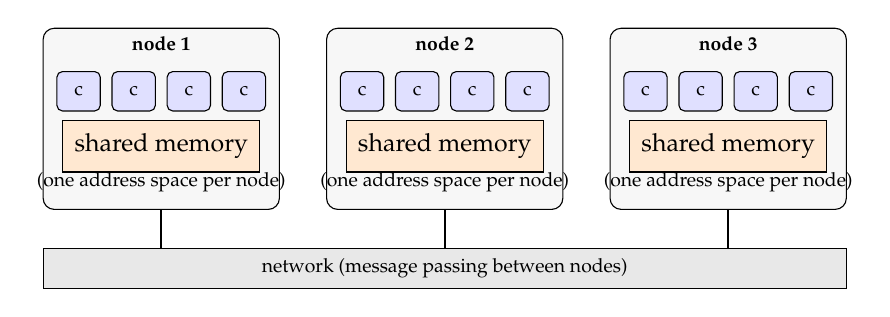
\begin{tikzpicture}
  \foreach \k/\x in {1/0, 2/3.6, 3/7.2} {
    \node[draw,rounded corners,fill=gray!6,minimum width=3.0cm,minimum height=2.3cm] (nd\k) at (\x,1.0) {};
    \node[font=\scriptsize\bfseries] at (\x,1.95) {node \k};
    \foreach \c in {-1.05,-0.35,0.35,1.05} { \node[pe,minimum width=5.5mm,minimum height=5mm,font=\scriptsize] at (\x+\c,1.35) {c}; }
    \node[mm,minimum width=2.5cm] at (\x,0.65) {shared memory};
    \node[font=\scriptsize] at (\x,0.2) {(one address space per node)};
  }
  \node[busbar,minimum width=10.2cm] (net) at (3.6,-0.9) {network (message passing between nodes)};
  \foreach \x in {0,3.6,7.2} \draw[lnk] (\x,-0.15) -- (\x,-0.65);
\end{tikzpicture}
\end{center}

\subsection{Comparison}

\begin{center}
\small
\begin{tabularx}{\linewidth}{@{}l X X X@{}}
\toprule
 & \textbf{UMA} & \textbf{NUMA} & \textbf{Distributed memory}\\
\midrule
Address space & one, shared & one, shared & one \emph{per processor}\\
Access time & same for all memory & local fast, remote slower & local only; remote by message\\
Communication & implicit (loads/stores) & implicit (loads/stores) & explicit (send/receive)\\
Cache coherence hardware & yes & yes (cc-NUMA) & not across nodes\\
Typical programming & threads, OpenMP & threads, OpenMP (NUMA-aware) & MPI\\
Scalability & tens of processors & hundreds & thousands and more\\
\bottomrule
\end{tabularx}
\end{center}

\begin{keyidea}
The first classification (Flynn) says how the \emph{work} is organised; the second says how the \emph{memory} is organised. A modern
cluster is MIMD, and it is shared-memory inside each node and distributed-memory between nodes.
\end{keyidea}

\section*{Exercises}
\addcontentsline{toc}{section}{Exercises}
\begin{enumerate}[label=\textbf{\thechapter.\arabic*},leftmargin=*]
  \item Classify each as SISD, SIMD, MISD or MIMD: (a) an AVX instruction adding two vectors of eight doubles;
        (b) eight MPI processes each running the same program on a different part of an array; (c) a quad-core
        laptop running four different programs; (d) a single-core, single-threaded program.
  \item Two threads each execute \cl{x = x + 1} on a shared variable that starts at $0$. List all final values of
        $x$ that can occur, and explain how.
  \item Is a two-socket server with one memory bank per socket a shared-memory or a distributed-memory machine? Explain
        in two sentences what distinguishes it from a cluster of two single-socket servers.
  \item A \cl{for} loop over an array of 1000 elements uses AVX with 4 doubles per instruction. How many vector
        instructions does the loop need, ignoring loop overhead? What if the loop body contains a data-dependent
        \cl{if/else}?
  \item On a two-socket NUMA machine, thread~0 allocates and initialises a 2~GB array, then 16 threads
        (8 per socket) process it in parallel. Explain why this can be slower than expected and how to fix it.
\end{enumerate}
\chapter{Caches and Cache Coherence}
\label{ch:coherence}

\newcommand{\Cread}{\textit{C\_read}}
\newcommand{\Cwrite}{\textit{C\_write}}

Shared memory is attractive because processors communicate through ordinary reads and writes. But
every modern processor has caches, and caches break the simple picture of ``one memory that everybody sees''.
This chapter explains how, and how hardware repairs it.

\section{Caches in a multiprocessor}
\slides{8--9}

Recall from your Chapter~1 that a cache holds \emph{copies} of small blocks of main memory, called
\term{cache lines} (or blocks), which are the unit of transfer between memory and cache. On current
processors a line is $64$~bytes. A read that finds its line in the cache is a \emph{hit} and takes a few cycles; one that does not is a
\emph{miss}, and the whole line is fetched from the next level.

In a multicore chip each core has its \emph{own private} cache (typically at least the first level, often also the second), and there may be a shared last-level cache. The private caches are where the trouble comes from.

\begin{center}
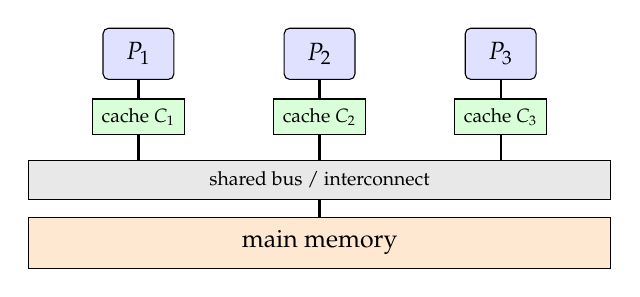
\begin{tikzpicture}
  \foreach \i in {1,2,3} {
     \node[pe] (p\i) at (\i*2.3,2.4) {$P_\i$};
     \node[ca] (c\i) at (\i*2.3,1.6) {cache $C_\i$};
     \draw[lnk] (p\i) -- (c\i);
  }
  \node[busbar,minimum width=7.4cm] (bus) at (4.6,0.8) {shared bus / interconnect};
  \node[mm,minimum width=7.4cm] (mem) at (4.6,0) {main memory};
  \foreach \i in {1,2,3} \draw[lnk] (c\i) -- (c\i |- bus.north);
  \draw[lnk] (bus) -- (mem);
\end{tikzpicture}
\end{center}

\subsection{Write policies: what happens on a write?}
\label{sec:writepolicy}

Reads are simple: if the line is in the cache, use it. Writes raise a question: the cache now holds a
\emph{newer} value than main memory. What should happen to memory? There are two classical answers.

\begin{definition}{write-through and write-back}
\textbf{Write-through}: every write updates the cache \emph{and} main memory immediately. Memory is never out of
date, but every write generates memory traffic.\\
\textbf{Write-back}: a write updates only the cache and sets a \term{dirty bit} on that line to record that it
differs from memory. The line is written back to memory only later, when it is \emph{evicted} (thrown out to make room for another
line). Repeated writes to the same line then cost nothing extra.
\end{definition}

Most caches are write-back, because it saves a great deal of memory bandwidth. A related detail: on a
\emph{write miss}, a write-back cache usually first fetches the whole line (\emph{write-allocate}) and then modifies it,
since the rest of the line must be valid in the cache. We will see that the ``Dirty'' state in the coherence protocol
below is the multiprocessor version of this dirty bit.

\begin{intuition}
Imagine a shared recipe book in the library (main memory) and a photocopy of one page on your desk (your cache). If you
scribble a correction on your copy, the library's page does not change until you walk back and
update it (write-back). Meanwhile a friend with their own photocopy of the same page has no idea about your correction. This is the problem
of the next section.
\end{intuition}

\section{The cache coherence problem}
\slides{9--10}

\begin{workedex}{stale data}
A variable $X$ is in main memory with the value $0$.
\begin{center}
\small
\begin{tabular}{@{}clccc@{}}
\toprule
Step & Event & $P_1$'s cache & $P_2$'s cache & Memory\\
\midrule
0 & initially & --- & --- & $X=0$\\
1 & $P_1$ reads $X$ (miss, line fetched) & $X=0$ & --- & $X=0$\\
2 & $P_2$ reads $X$ (miss, line fetched) & $X=0$ & $X=0$ & $X=0$\\
3 & $P_1$ writes $X=1$ (hit, only cache updated) & $X=1$ & $X=0$ & $X=0$\\
4 & $P_2$ reads $X$ (\textbf{hit}) returns \textbf{0} & $X=1$ & $X=0$ & $X=0$\\
\bottomrule
\end{tabular}
\end{center}
In step~4, $P_2$ hits in its own cache and gets $0$, although the latest value written is $1$. The slide marks
exactly this: ``Cache hit: wrong data!!''. The value $0$ in $P_2$'s cache is called \term{stale}.
\end{workedex}

\begin{pitfall}
Write-through does not solve this. With write-through, memory would hold $1$ after step~3, but $P_2$'s \emph{copy} would still say $0$ and
$P_2$ would still hit on it. The problem is not main memory but the existence of \emph{several copies}.
\end{pitfall}

\begin{definition}{cache coherence}
A memory system is \emph{coherent} if, for every individual memory location, the following hold:
\begin{enumerate}
  \item \textbf{Program order.} A read by a processor that follows its own write to the location returns that
        write's value (unless another processor wrote in between).
  \item \textbf{Coherent view.} A read returns a value written by another processor if the write happened
        ``long enough ago'': writes do not stay invisible forever.
  \item \textbf{Write serialisation.} Writes to the same location are seen in the \emph{same order} by all
        processors. If $P_1$ writes $1$ and $P_2$ writes $2$, it cannot happen that one processor sees $1$ then $2$
        while another sees $2$ then $1$.
\end{enumerate}
The slide's one-line version: processes shouldn't read ``stale'' data.
\end{definition}

\begin{keyidea}
A coherent system behaves, \emph{per location}, as if there were just one copy of that location.
\end{keyidea}

\begin{pitfall}
\textbf{Coherence is not consistency.} Coherence is about the order of operations on \emph{one} location.
\emph{Memory consistency} is about the order in which operations on \emph{different} locations become visible, and it
is what programs depend on in code like this (initially \cl{data = flag = 0}):
\begin{center}
\begin{tabular}{@{}l|l@{}}
$P_1$ & $P_2$\\ \hline
\cl{data = 42;} & \cl{while (flag == 0) ;}\\
\cl{flag = 1;} & \cl{print(data);}\\
\end{tabular}
\end{center}
You would expect $42$ to be printed; whether this is guaranteed depends on the machine's \emph{consistency model}.
Consistency models are a separate topic that this course does not examine in depth. Everything below concerns coherence only.
\end{pitfall}

\textbf{Who fixes it?} In principle software could do it: the compiler or operating system could mark shared data as uncacheable or
flush caches at the right times. This would be slow and a nightmare to program. The
slides give the standard answer: \emph{hardware} coherence mechanisms, invisible to the program.

\section{Update versus invalidate}
\slides{11--12}

When a processor writes a line that other caches also hold, those other copies must be dealt with. There are two policies:

\begin{definition}{write-update and write-invalidate}
\textbf{Write-update}: on every write, the new value is broadcast to all caches holding the line, and they
overwrite their copies. \\
\textbf{Write-invalidate}: on a write, the writer sends a short message that makes the other caches mark their copies
\emph{invalid}. A processor that later needs the line takes a miss and fetches the fresh value.
\end{definition}

The slide asks: which is better? Compare them on two access patterns.

\begin{workedex}{one writer, no readers}
$P_1$ writes the same variable $100$ times in a row; $P_2$ holds a copy but never looks at it again.
\begin{itemize}
  \item \textbf{Update:} $100$ broadcasts, each carrying data, although nobody needs them.
  \item \textbf{Invalidate:} the first write invalidates $P_2$'s copy ($1$ message). $P_1$ now holds the only valid copy,
        and the other $99$ writes hit locally with no bus traffic at all.
\end{itemize}
\end{workedex}

\begin{workedex}{tight producer--consumer}
$P_1$ writes a value, $P_2$ reads it, $P_1$ writes the next value, $P_2$ reads it, and so on.
\begin{itemize}
  \item \textbf{Update:} each write is broadcast and $P_2$'s read hits. One transaction per round, with a fast read.
  \item \textbf{Invalidate:} each write invalidates $P_2$'s copy, and $P_2$'s read then misses and must fetch the line.
        Two transactions per round and a slow read.
\end{itemize}
\end{workedex}

\begin{center}
\small
\begin{tabularx}{\linewidth}{@{}l X X@{}}
\toprule
 & \textbf{Write-update} & \textbf{Write-invalidate}\\
\midrule
Write cost & high: data broadcast on every write & low: a short invalidation, and only for the first write\\
Read after a remote write & fast: copy already updated & slow: miss, fetch the line\\
Wasted traffic & updates to caches that never read again & none for data that is not re-read\\
Multi-word lines & each word written is a separate update & one invalidation covers the whole line\\
Best for & one-to-one producer--consumer on a single word & most real programs\\
\bottomrule
\end{tabularx}
\end{center}

Most programs write a variable many times before anyone else reads it, and data is usually written in
runs to neighbouring words of the same line, so \textbf{write-invalidate dominates in practice} and is what the
rest of the course (and almost all hardware) assumes.

\section{The three-state invalidate protocol}
\slides{12--14}

A coherence \term{protocol} is a set of rules that every cache controller follows so that the whole system stays coherent. It works
line by line: \emph{each line in each cache} has a \emph{state}, and the state changes in response to events.
Note: the state belongs to the pair (cache, line), not to a variable or to a processor in general.

\subsection{The states}

The slides use three states (the textbook name for this protocol is \textbf{MSI}, with Modified
for the slide's Dirty):

\begin{definition}{the three states}
\textbf{I -- Invalid}: this cache has no valid copy of the line (it was never loaded or another processor has updated the data).\\
\textbf{S -- Shared}: this cache has a valid copy, \emph{read-only}, and other caches may also have copies. Memory is up to date.\\
\textbf{D -- Dirty} (Modified in textbooks): this cache has the \emph{only} valid copy and it has been modified. Memory is
\emph{stale}.
\end{definition}

\begin{keyidea}
The protocol maintains the \emph{single-writer, multiple-reader} rule. For any line, at any moment either
(a) any number of caches hold it in S (and none in D), or (b) exactly one cache holds it in D and all others have it invalid.
\end{keyidea}

\subsection{The events}

Two kinds of events change a line's state:
\begin{itemize}
  \item \textbf{Events from this cache's own processor}: \emph{read} and \emph{write}.
  \item \textbf{Events observed from other processors} (the dashed arrows in the slide's diagram):
        \Cread{} means ``another processor is reading this line'', and \Cwrite{} means ``another processor is writing
        this line'' (it wants exclusive ownership).
\end{itemize}

\subsection{The state diagram}

\begin{center}
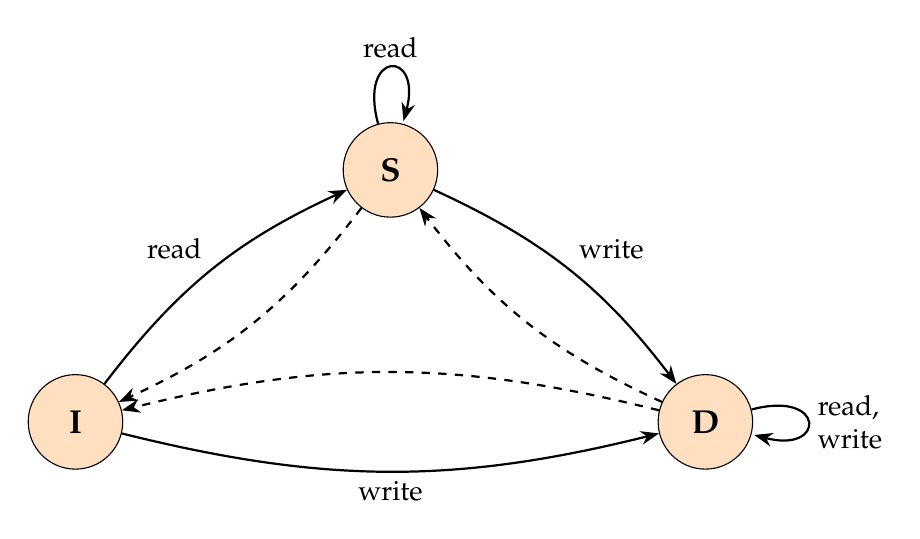
\begin{tikzpicture}[st/.style={circle,draw,fill=orange!25,minimum size=12mm,font=\bfseries\large},scale=1.0]
  \node[st] (S) at (0,3.2) {S};
  \node[st] (I) at (-4,0) {I};
  \node[st] (D) at (4,0) {D};
  \path[->,thick]
    (S) edge[loop above] node[above]{read} (S)
    (D) edge[loop right] node[right,align=left]{read,\\write} (D)
    (I) edge[bend left=14] node[above left]{read} (S)
    (S) edge[bend left=14] node[above right]{write} (D)
    (I) edge[bend right=14] node[below]{write} (D);
  \path[->,thick,dashed]
    (S) edge[bend left=14] node[above left]{\Cwrite} (I)
    (D) edge[bend left=14] node[below right]{\Cread} (S)
    (D) edge[bend right=14] node[above]{\Cwrite} (I);
\end{tikzpicture}
\end{center}

Solid arrows are caused by this cache's own processor; dashed arrows are caused by what \emph{other} processors do.
(Events not drawn leave the state unchanged: for example, \Cread{} on a line in S keeps it in S, and \Cread{} or
\Cwrite{} on a line in I does nothing.)

\subsection{Reading the diagram, one arrow at a time}

\begin{center}
\small
\begin{tabularx}{\linewidth}{@{}c l c X@{}}
\toprule
\textbf{From} & \textbf{Event} & \textbf{To} & \textbf{What the hardware does}\\
\midrule
S & read & S & Hit. Nothing leaves the cache.\\
S & write & D & The cache must become the sole owner. It broadcasts an \emph{invalidate}; every other copy goes S$\to$I (their \Cwrite{}). No data transfer is needed, since this cache already holds the line.\\
S & \Cwrite & I & Another processor is writing: drop this copy.\\
I & read & S & Read miss. The line is fetched from memory, or from the cache that holds it in D (see below). Cache ends in S.\\
I & write & D & Write miss. The line is fetched \emph{with intent to modify}, all other copies are invalidated, and the cache ends in D.\\
D & read, write & D & Hits. This cache is the sole owner, so no bus traffic at all.\\
D & \Cread & S & Another processor wants to read. This cache holds the only up-to-date data, so it \emph{supplies} the line (and memory is updated); both caches then hold the line in S.\\
D & \Cwrite & I & Another processor wants to write. This cache supplies the data and invalidates its own copy: the other cache becomes the single owner (D).\\
\bottomrule
\end{tabularx}
\end{center}

\begin{pitfall}
When a line is Dirty somewhere, \emph{memory is stale}. A processor that misses on such a line must \textbf{not} read it from memory; it must get it from the owning
cache. This is why the transitions D$\to$S and D$\to$I involve the owner supplying data.
\end{pitfall}

\subsection{A complete trace}

\begin{workedex}{two processors, one variable}
Line containing $X$ is in memory with $X=0$; both caches start in I. Write-back, as above.
\begin{center}
\small
\begin{tabular}{@{}cllllll@{}}
\toprule
 & Event & $P_1$ & $P_2$ & Memory & Bus activity\\
\midrule
0 & start & I & I & $0$ & ---\\
1 & $P_1$ reads $X$ & S ($0$) & I & $0$ & read miss, line from memory\\
2 & $P_2$ reads $X$ & S ($0$) & S ($0$) & $0$ & read miss, line from memory\\
3 & $P_1$ writes $X{=}5$ & D ($5$) & I & $0$ (stale) & invalidate sent; $P_2$: S$\to$I\\
4 & $P_2$ reads $X$ & S ($5$) & S ($5$) & $5$ & read miss; $P_1$ (D) supplies line, D$\to$S\\
5 & $P_2$ writes $X{=}7$ & I & D ($7$) & $5$ (stale) & invalidate sent; $P_1$: S$\to$I\\
6 & $P_1$ reads $X$ & S ($7$) & S ($7$) & $7$ & read miss; $P_2$ (D) supplies line, D$\to$S\\
\bottomrule
\end{tabular}
\end{center}
Notice that step~4 returns $5$, not the stale $0$, and step~6 returns $7$: coherence is restored. The invariant (single writer or many
readers) holds after every step. Steps~3 and 5 have the memory stale; no processor can read it by mistake,
because a processor that misses is served by the owner.
\end{workedex}

\subsection{Beyond three states (not on the slides, but you will meet the names)}

\begin{itemize}
  \item \textbf{MESI} adds \textbf{E (Exclusive)}: a clean line that this cache holds and no other cache does. It matters
        because most data is private. In MSI, reading a private line then writing it needs two steps: I$\to$S on the read, then an
        invalidation broadcast on the write. In MESI the read brings the line in as E, and the first write moves E$\to$D \emph{silently},
        with no bus transaction.
  \item \textbf{MOESI} adds \textbf{O (Owned)}: a dirty line that is shared. The owner supplies data to readers and
        memory need not be updated at every read, saving memory traffic.
\end{itemize}

\textbf{A caution about the diagram.} It shows transitions as if they were instantaneous. In real hardware two processors may try to write
the same line at the same time, and the controllers must order these events consistently. This is exactly what the bus provides in a snooping system (next
section) and what the directory does in a directory system.

\section{Implementing coherence: snooping and directories}
\slides{15--17}

The protocol is the \emph{rules}; the \emph{implementation} decides how cache controllers learn about each other's actions.
There are two main designs.

\subsection{Snooping (bus-based)}

\begin{definition}{snooping protocol}
All caches are attached to a \emph{shared bus}. Every memory operation that matters for coherence
(a miss, an invalidation) is \emph{broadcast on the bus}. Each cache controller continuously watches (``snoops on'') the bus, compares each address against the lines in its own cache, and takes action when it
holds a copy.
\end{definition}

Why this works: the slide says ``there is only one operation through the bus at a time''. The bus is a single shared wire set, so it
automatically puts all transactions in a single order that everyone sees, which gives write serialisation for free. When $P_1$ puts an
invalidation for line $L$ on the bus, every other controller hears it in the same order, invalidates its copy of $L$ if it has one, and
the protocol of the previous section proceeds.

\textbf{Limitations.}
\begin{itemize}
  \item The bus carries one transaction at a time, so it becomes a \emph{bottleneck} as processors are added: every miss and
        invalidation from every processor competes for it.
  \item Every cache must check every bus transaction, which costs energy and cache bandwidth even for lines it does not have.
  \item Electrically, a bus with many attached devices cannot be clocked fast.
\end{itemize}
Snooping is therefore used for small machines (roughly up to a few tens of processors) or within a small group of cores.

\subsection{Directory-based}

\begin{definition}{directory protocol}
A \emph{directory} records, for each memory line, \emph{which caches currently hold a copy} (and whether it is
dirty). On a miss or a write, coherence messages are sent \emph{only to the caches the directory lists}, instead of being
broadcast to everyone.
\end{definition}

The slide says ``a central directory maintains states of cache blocks, associated processors''. Logically there is one directory; in a
large machine it is \emph{physically distributed}, each node keeping the directory entries for the lines in \emph{its own} memory
(the line's \term{home node}). A single physical directory would itself be a bottleneck.

\textbf{Directory entry.} For each line: a state (uncached, shared, or exclusive/dirty) and the
\term{presence bits}: one bit per processor, $1$ if that processor has a copy.

\textbf{How a write to a shared line works.} Suppose a line is cached by $P_2$ and $P_3$, and $P_1$ wants to write it.

\begin{center}
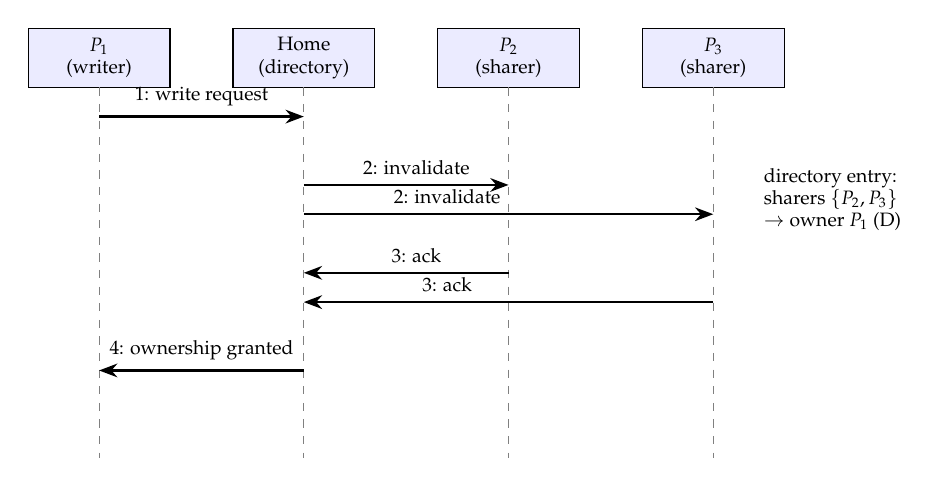
\begin{tikzpicture}[x=2.6cm,y=0.62cm]
  \foreach \x/\n in {0/{$P_1$\\(writer)}, 1/{Home\\(directory)}, 2/{$P_2$\\(sharer)}, 3/{$P_3$\\(sharer)}} {
    \node[draw,fill=blue!8,minimum width=18mm,font=\scriptsize,align=center] (h\x) at (\x,0) {\n};
    \draw[dashed,gray] (\x,-0.6) -- (\x,-8.2);
  }
  \draw[->,thick] (0,-1.2) -- node[above,font=\scriptsize]{1: write request} (1,-1.2);
  \draw[->,thick] (1,-2.6) -- node[above,font=\scriptsize,pos=0.55]{2: invalidate} (2,-2.6);
  \draw[->,thick] (1,-3.2) -- node[above,font=\scriptsize,pos=0.35]{2: invalidate} (3,-3.2);
  \draw[->,thick] (2,-4.4) -- node[above,font=\scriptsize,pos=0.45]{3: ack} (1,-4.4);
  \draw[->,thick] (3,-5.0) -- node[above,font=\scriptsize,pos=0.65]{3: ack} (1,-5.0);
  \draw[->,thick] (1,-6.4) -- node[above,font=\scriptsize]{4: ownership granted} (0,-6.4);
  \node[font=\scriptsize,align=left,anchor=west] at (3.2,-2.9) {directory entry:\\ sharers $\{P_2,P_3\}$\\ $\rightarrow$ owner $P_1$ (D)};
\end{tikzpicture}
\end{center}

Only $P_2$ and $P_3$ are bothered. With $64$ processors a snooping system would have interrupted all $63$ others. In
a \emph{read miss on a line that is dirty in another cache}, the request goes to the home, the home \emph{forwards} it to the
owner, and the owner sends the data to the requester: three steps (hops) instead of the bus's one broadcast. This indirection
is the price paid for scalability.

\subsection{How big is the directory?}

With one presence bit per processor per line (the \term{full bit vector} scheme in the slide), the directory needs
$P$ bits for each of the $M$ memory lines: storage proportional to $M\times P$.

\begin{workedex}{directory overhead}
Memory of $64$~GiB with $64$-byte ($512$-bit) lines has $M = 2^{36}/2^{6} = 2^{30}$ lines.
\begin{itemize}
  \item $P=64$ processors: $2^{30}\times 64$ bits $=8$~GiB, an overhead of $64/512 = 12.5\%$.
  \item $P=1024$ processors: $2^{30}\times 1024$ bits $=128$~GiB, an overhead of $1024/512 = 200\%$: the directory is \emph{larger than the data}.
\end{itemize}
The overhead per line is $P/512$, so it grows linearly with the number of processors. That is the ``but not necessary'' of the slide.
\end{workedex}

\textbf{Why most of that storage is wasted, and the fix.} The total capacity of all caches is tiny compared with memory, so at any moment
\emph{almost every line is in no cache at all} and most of the directory is rows of zeros. And lines that are cached are typically
cached by only a handful of processors. The slide's ``sparse or tagged directory'' and ``limited cache lines and limited presence bits''
exploit this:
\begin{itemize}
  \item \textbf{Sparse (tagged) directory}: keep entries only for lines that are currently cached somewhere, in a small table
        looked up by the line's address (like a cache for directory entries), instead of one entry per memory line.
  \item \textbf{Limited presence information}: instead of $P$ bits, store the identities of at most $k$ sharers (say $k=4$,
        which costs $k\log_2 P$ bits). If a fifth processor wants a copy, the protocol either invalidates one existing sharer, or
        switches to broadcast for that line, or uses a coarse vector (one bit per \emph{group} of processors).
\end{itemize}

\subsection{Snooping versus directory}

\begin{center}
\small
\begin{tabularx}{\linewidth}{@{}l X X@{}}
\toprule
 & \textbf{Snooping} & \textbf{Directory}\\
\midrule
Who learns about a write & everybody (broadcast) & only the listed sharers\\
Interconnect & shared bus (one transaction at a time) & any network, many transactions in parallel\\
Order of writes & provided by the bus & provided by the home node\\
Latency of a miss & short (broadcast) & longer (indirection through the home)\\
Extra storage & none (just the state bits in the caches) & directory ($\propto$ lines $\times$ sharer information)\\
Scalability & tens of processors & hundreds to thousands\\
\bottomrule
\end{tabularx}
\end{center}

Modern multi-socket servers and many-core chips typically use a hybrid: snooping within a small group of cores that
share a cache or a ring, and directory-like structures (or ``snoop filters'') to avoid broadcasting to the rest.

\section{False sharing}
\slides{18--19}

\subsection{The problem}

The protocol operates on whole cache lines. The unit of ownership is a \emph{line} ($64$ bytes), not a variable (typically $4$ or $8$
bytes). The hardware has no idea that a line contains eight different variables.

\begin{definition}{false sharing}
Two processors repeatedly access \emph{different} variables that happen to lie in the \emph{same cache line}, and at least one of them writes.
Logically they share nothing, but the coherence hardware treats the line as shared and moves it back and forth.
\end{definition}

\begin{center}
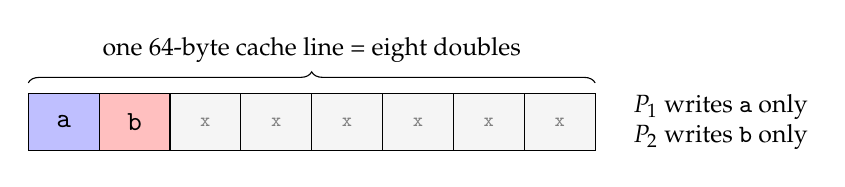
\begin{tikzpicture}[x=0.9cm,y=0.9cm]
  \foreach \i in {0,...,7} { \draw[fill=gray!8] (\i,0) rectangle (\i+1,0.8); }
  \draw[fill=blue!25] (0,0) rectangle (1,0.8); \node at (0.5,0.4) {\cl{a}};
  \draw[fill=red!25]  (1,0) rectangle (2,0.8); \node at (1.5,0.4) {\cl{b}};
  \foreach \i in {2,...,7} \node[font=\scriptsize,gray] at (\i+0.5,0.4) {\cl{x}};
  \draw[decorate,decoration={brace,amplitude=4pt}] (0,0.95) -- (8,0.95) node[midway,above=4pt,font=\small]{one 64-byte cache line = eight doubles};
  \node[font=\small,align=left,anchor=west] at (8.4,0.4) {$P_1$ writes \cl{a} only\\$P_2$ writes \cl{b} only};
\end{tikzpicture}
\end{center}

\begin{workedex}{the line ping-pongs}
$P_1$ repeatedly writes \cl{a} and $P_2$ repeatedly writes \cl{b}, in the same line, with the invalidate protocol:
\begin{enumerate}
  \item $P_1$ writes \cl{a}: line in $P_1$ is D, in $P_2$ is I.
  \item $P_2$ writes \cl{b}: a write miss. The line must be fetched from $P_1$; now $P_2$ is D and $P_1$ is I.
  \item $P_1$ writes \cl{a} again: again a write miss. The line moves back to $P_1$. And so on.
\end{enumerate}
Every write is a miss that needs a transfer across the interconnect (tens to hundreds of cycles) instead of a hit
(a few cycles). The program is correct but can be several times slower than it should be, and it often gets \emph{slower} as threads are added.
\end{workedex}

\textbf{True versus false sharing.} If the two processors accessed the \emph{same} word, the communication would be real
(\emph{true sharing}) and unavoidable. False sharing is an artifact of data layout, and therefore it can be removed.

\subsection{An example in code}

A very common way to get false sharing: each thread keeps its running total in its own element of a shared array.

\begin{lstlisting}
#define NT 8
double partial[NT];                       /* 8 doubles = 64 bytes = ONE cache line */

#pragma omp parallel num_threads(NT)
{
    int t = omp_get_thread_num();
    for (long i = t*(N/NT); i < (t+1)*(N/NT); i++)
        partial[t] += a[i];               /* every iteration writes the shared line */
}
\end{lstlisting}

All eight elements of \cl{partial} sit in one line. Every update by any thread invalidates the line in the other seven caches.
Two fixes:

\begin{lstlisting}
/* Fix 1 (best): accumulate in a private variable, write once at the end */
{   double local = 0.0;
    for (long i = t*(N/NT); i < (t+1)*(N/NT); i++) local += a[i];
    partial[t] = local;                   /* one write per thread */
}

/* Fix 2: padding - make each thread's slot occupy its own cache line */
typedef struct { double v; char pad[56]; } padded_t;      /* sizeof = 64 bytes */
_Alignas(64) padded_t partial2[NT];
/* ... partial2[t].v += a[i]; ... */
\end{lstlisting}

\begin{pitfall}
Optimising compilers often keep \cl{partial[t]} in a register for the whole loop, which would hide the effect in the first
version. False sharing shows up when the stores really reach memory. Also, \cl{\_Alignas(64)} is needed: padding to $64$ bytes
only helps if the array itself starts on a line boundary.
\end{pitfall}

\subsection{The slide's example: a Fortran matrix}

Fortran stores a matrix in \term{column-major} order: the elements of one column are consecutive in memory
(C is \term{row-major}: elements of a row are consecutive). So in Fortran, $A(1,j), A(2,j), A(3,j),\dots$ are neighbours.

Suppose thread $t$ is responsible for \emph{row} $t$ and updates $A(t,1), A(t,2),\ldots$ Each thread walks along its row, but
at any step the threads touch $A(1,j), A(2,j),\ldots, A(8,j)$, eight neighbours in the \emph{same column}, hence the same cache line:

\begin{center}
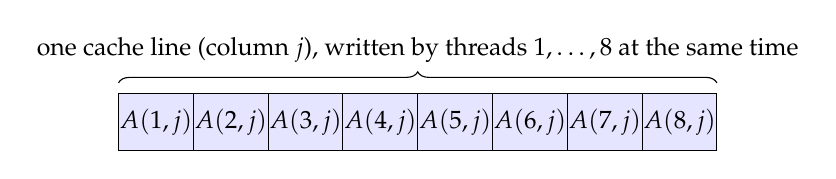
\begin{tikzpicture}[x=0.95cm,y=0.9cm]
  \foreach \i in {1,...,8} { \draw[fill=blue!10] (\i-1,0) rectangle (\i,0.8); \node at (\i-0.5,0.4) {\small $A(\i,j)$}; }
  \draw[decorate,decoration={brace,amplitude=4pt}] (0,0.95) -- (8,0.95) node[midway,above=4pt,font=\small]{one cache line (column $j$), written by threads $1,\dots,8$ at the same time};
\end{tikzpicture}
\end{center}

That is false sharing in its worst form.

\textbf{The slide's remedy.} Reorganise so that each thread works on a \emph{set of consecutive rows}. In a column, a block of consecutive rows
is contiguous in memory, so a thread's data forms long contiguous runs and different threads' runs only meet at the block boundaries.
A boundary can still fall inside a line (``overlapping of cache lines if matrix size not divisible by processors''). \emph{Padding} fixes this: add
dummy elements so the block size is a multiple of the line size.

\begin{workedex}{padding the number of rows}
A matrix has $n=100$ rows of doubles ($8$ bytes), $p=4$ threads, $64$-byte lines (8 doubles per line), and the array starts on a line boundary.
\begin{itemize}
  \item Without padding: each thread gets $25$ rows, which is $200$ bytes $=3.125$ lines. The block boundaries fall inside lines, so
        neighbouring threads share lines. (Moreover a column is $800$~bytes $=12.5$ lines, so columns are not line-aligned either.)
  \item With padding: round the per-thread block up to a multiple of $8$ rows, $25\to 32$, and allocate $4\times 32 = 128$ rows
        (the last $28$ rows are dummy). Each thread's block is $256$ bytes $=4$ whole lines and a column is $1024$~bytes
        $=16$ lines, so each column starts on a line boundary and no line is shared between threads.
\end{itemize}
The price is $28\%$ extra memory; padding trades memory for speed. The same idea applies to C, with the roles of rows and columns swapped.
\end{workedex}

\begin{keyidea}
Coherence works on \emph{lines}. To avoid false sharing, give each thread data that is contiguous and (if possible) aligned to line boundaries,
and keep frequently written per-thread data in private variables instead of neighbouring slots of a shared array. Tools such as Linux
\cl{perf c2c} can detect it.
\end{keyidea}

\section*{Exercises}
\addcontentsline{toc}{section}{Exercises}
\begin{enumerate}[label=\textbf{\thechapter.\arabic*},leftmargin=*]
  \item Three processors $P_1,P_2,P_3$ all start with a line in state I. Using the three-state protocol, give the state of the line in each
        cache after each step: (a) $P_1$ writes; (b) $P_2$ reads; (c) $P_2$ writes; (d) $P_3$ reads; (e) $P_1$ reads.
  \item $P_1$ writes a variable $50$ times in a row, then $P_2$ reads it once. Count the bus transactions under write-update
        and under write-invalidate (count each broadcast, invalidation and read miss as one).
  \item A system has $256$ processors and $128$-byte cache lines. What is the percentage overhead of a full bit-vector directory?
  \item Four threads each increment their own \cl{int} counter, stored in \cl{int c[4]}. How many cache lines hold the array
        (assume it is $64$-byte aligned)? How much would you pad each counter, and how much memory would the padded array use?
  \item Explain why read-only shared data causes no coherence traffic after the first misses.
  \item A column-major matrix has $n=100$ rows, $p=8$ threads and $64$-byte lines. Following the slide's approach,
        choose the padded number of rows.
\end{enumerate}
\chapter{Interconnection Networks}
\label{ch:networks}

Whatever the memory organisation, processors (or processors and memory) have to be \emph{connected}. In a
shared-memory machine the interconnect joins processors to memory modules; in a distributed-memory machine it joins
processors to each other. As machines grow, the interconnect is often what limits performance, so it deserves careful study.

\section{What an interconnect is made of}
\slides{20--22}

An interconnect has a few kinds of building blocks.

\begin{definition}{network interface, link, switch}
A \textbf{network interface} connects a processor (or memory) to the network. In a cluster this is the network card, attached to the
processor over PCI or PCI-e, the expansion bus of the computer. A \textbf{link} is a set of wires or an optical fibre carrying data between two points.
A \textbf{switch} has several input \emph{ports} and output \emph{ports} and forwards data arriving on an input to the appropriate
output. The number of ports is the switch's \emph{degree}.
\end{definition}

The slide describes the \term{communication network} as switching elements to which the processors are attached through ports; the switching elements are linked
in some \emph{pattern}, and that pattern is the \term{topology}. (In shared-memory machines the memory modules are
attached to the network too.)

It helps to think of the whole interconnect as a \emph{graph}: the nodes are processors, memories and switches, and the edges are links. A \emph{hop} is one link traversed,
and the \emph{distance} between two nodes is the number of links on the shortest path between them.

\section{Static and dynamic networks}
\slides{23--24}

\begin{definition}{static (direct) network}
Fixed, point-to-point links connect the processing nodes directly to each other. Each node can be thought of as a processor
together with its own small switch (router). Examples: ring, mesh, torus, hypercube.
\end{definition}

\begin{definition}{dynamic (indirect) network}
Processors (and memories) are attached to \emph{switches}, and the switches make connections on demand. Paths are
formed dynamically by setting the switches. Examples: crossbar, Omega network, fat tree.
\end{definition}

\begin{center}
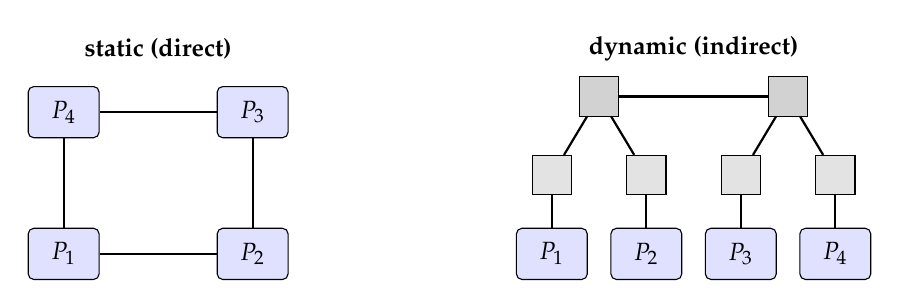
\begin{tikzpicture}
  % static
  \node[font=\small\bfseries] at (1.2,2.6) {static (direct)};
  \foreach \i/\x/\y in {1/0/0, 2/2.4/0, 3/2.4/1.8, 4/0/1.8} {
     \node[pe] (a\i) at (\x,\y) {$P_\i$};
  }
  \draw[lnk] (a1) -- (a2) -- (a3) -- (a4) -- (a1);
  % dynamic
  \node[font=\small\bfseries] at (8,2.6) {dynamic (indirect)};
  \foreach \i/\x in {1/6.2,2/7.4,3/8.6,4/9.8} {
     \node[pe] (b\i) at (\x,0) {$P_\i$};
     \node[swt] (s\i) at (\x,1.0) {};
     \draw[lnk] (b\i) -- (s\i);
  }
  \node[swt,fill=gray!35] (t1) at (6.8,2.0) {}; \node[swt,fill=gray!35] (t2) at (9.2,2.0) {};
  \draw[lnk] (s1) -- (t1) -- (s2); \draw[lnk] (s3) -- (t2) -- (s4); \draw[lnk] (t1) -- (t2);
\end{tikzpicture}
\end{center}

\section{How a message travels: a cost model and routing}
\slides{23}

This section goes slightly beyond the slides, but it explains \emph{why} the quantities the slides define (diameter, bisection width) matter.

\subsection{A simple cost model}

Suppose a message of $m$ words crosses $l$ links. Three constants describe the machine:
$t_s$, the \emph{startup time} (software overhead and setting up the transfer, paid once per message, independent of $m$);
$t_h$, the time for the message's header to pass through one switch (per-hop delay);
and $t_w$, the time to transfer one word over a link ($1/t_w$ is the bandwidth).

\begin{itemize}
  \item \textbf{Store-and-forward}: each switch receives the whole message and only then forwards it:
        $T = t_s + l\,(t_h + m\,t_w)$.
  \item \textbf{Cut-through (wormhole) routing}: the message is cut into small pieces that are pipelined along the path, like cars on a road; the head
        moves on while the tail is still leaving the source: $T = t_s + l\,t_h + m\,t_w$.
\end{itemize}

\begin{workedex}{store-and-forward versus cut-through}
$m=1000$ words, $t_w=1$, $t_h=10$, $t_s=100$ (arbitrary time units), $l=5$ links.
\[
  T_{\text{SF}} = 100 + 5(10+1000) = 5150, \qquad T_{\text{CT}} = 100 + 5\cdot 10 + 1000 = 1150 .
\]
With cut-through, the long message pays the transfer time $m\,t_w$ only \emph{once}, and distance adds only a little.
\end{workedex}

Two lessons: for \emph{short} messages the startup and hop count dominate, so a small \emph{diameter} helps; for \emph{long}
messages the bandwidth term dominates. And whenever many messages must cross the same part of the network, the total traffic
divided by the available bandwidth across that cut is a lower bound on the time. That is what \emph{bisection bandwidth}
(below) measures.

\subsection{Routing}

\term{Routing} decides which path a message takes from source to destination (the slide: ``how the route taken by the message
from source to destination is decided'').
\begin{itemize}
  \item \textbf{Deterministic} routing always uses the same path for a given source and destination. A common form is
        \emph{dimension-ordered routing}: in a 2-D mesh, move along the $x$ direction until the column matches, then along $y$.
        It is simple and avoids \emph{deadlock} (a cycle of messages each waiting for a resource held by the next) on meshes.
  \item \textbf{Adaptive} routing chooses among several paths according to current congestion; it spreads load but is harder to build.
\end{itemize}

\section{Static topologies}
\slides{24, 28--31}

\subsection{Completely connected, star, linear array and ring}

\begin{center}
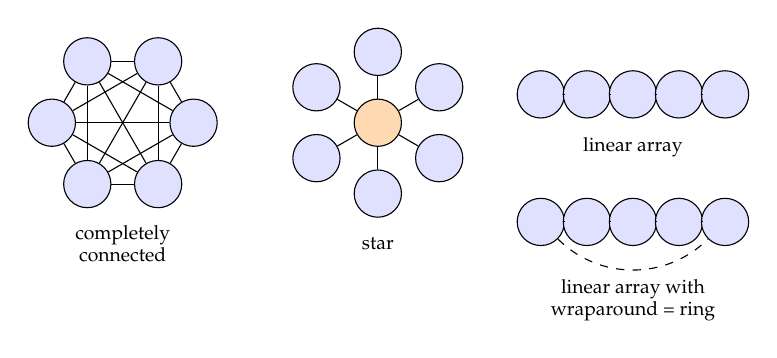
\begin{tikzpicture}[scale=0.9]
  % complete graph
  \foreach \i in {0,...,5} \node[dn] (k\i) at ({60*\i}:1) {};
  \begin{pgfonlayer}{background}
  \foreach \i in {0,...,5} \foreach \j in {0,...,5} { \ifnum\i<\j \draw (k\i) -- (k\j); \fi }
  \end{pgfonlayer}
  \node[font=\scriptsize,align=center] at (0,-1.7) {completely\\connected};
  % star
  \begin{scope}[shift={(3.6,0)}]
    \node[dn,fill=orange!30] (h) at (0,0) {};
    \foreach \i in {0,...,5} \node[dn] (s\i) at ({60*\i+30}:1) {};
    \begin{pgfonlayer}{background}\foreach \i in {0,...,5} \draw (h) -- (s\i);\end{pgfonlayer}
    \node[font=\scriptsize] at (0,-1.7) {star};
  \end{scope}
  % linear array
  \begin{scope}[shift={(5.9,0)}]
    \foreach \i in {0,...,4} \node[dn] (l\i) at (0.65*\i,0.4) {};
    \draw (l0) -- (l1) -- (l2) -- (l3) -- (l4);
    \node[font=\scriptsize] at (1.3,-0.35) {linear array};
    \foreach \i in {0,...,4} \node[dn] (r\i) at (0.65*\i,-1.4) {};
    \draw (r0) -- (r1) -- (r2) -- (r3) -- (r4);
    \draw[dashed] (r0) to[bend right=45] (r4);
    \node[font=\scriptsize,align=center] at (1.3,-2.5) {linear array with\\wraparound = ring};
  \end{scope}
\end{tikzpicture}
\end{center}

\begin{itemize}
  \item \textbf{Completely connected}: every node has a direct link to every other, so any message goes in one hop and
        no pair blocks another. It is the static counterpart of the crossbar, with the same flaw: the number of links is
        $p(p-1)/2$, which is hopeless for large $p$.
  \item \textbf{Star}: all nodes connect to a central node that acts as a switch. Diameter 2, but the central node is a bottleneck (similar to a bus).
  \item \textbf{Linear array}: nodes in a line, each linked to its two neighbours. A \textbf{ring} (also a ``1-D torus'') adds a
        \emph{wraparound} link between the two ends. The wraparound halves the diameter and doubles the number of routes.
\end{itemize}

\subsection{Meshes and tori}

\begin{center}
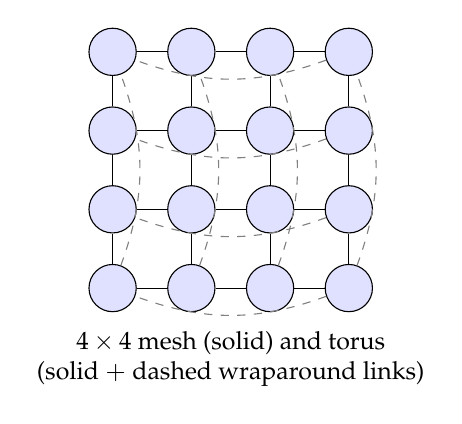
\begin{tikzpicture}
  \foreach \i in {0,...,3} \foreach \j in {0,...,3} { \node[dn] (m\i\j) at (1.0*\i,1.0*\j) {}; }
  \foreach \i in {0,...,3} \foreach \j in {0,...,2} { \draw (m\i\j) -- (m\i\the\numexpr\j+1\relax); }
  \foreach \i in {0,...,2} \foreach \j in {0,...,3} { \draw (m\i\j) -- (m\the\numexpr\i+1\relax\j); }
  \foreach \j in {0,...,3} \draw[dashed,gray] (m3\j) to[bend left=20] (m0\j);
  \foreach \i in {0,...,3} \draw[dashed,gray] (m\i0) to[bend right=20] (m\i3);
  \node[font=\small,align=center] at (1.5,-0.9) {$4\times4$ mesh (solid) and torus\\(solid $+$ dashed wraparound links)};
\end{tikzpicture}
\end{center}

A \term{2-D mesh} arranges $p$ nodes in a $\sqrt p\times\sqrt p$ grid; node $(i,j)$ is linked to $(i\pm1,j)$ and $(i,j\pm1)$.
It is easy to lay out on a chip or board (it is planar) and it maps naturally onto computations on grids (images, stencils). A \term{torus} adds wraparound
links in each dimension. Extending to three dimensions gives a 3-D mesh/torus, where interior nodes have $6$ neighbours; 3-D simulations map naturally onto it.

\begin{definition}{$k$-ary $d$-cube / $k$-$d$ mesh}
A network with $d$ dimensions and $k$ nodes along each dimension, so $p=k^{d}$ nodes. A linear array is $d=1$, a 2-D mesh $d=2$. With wraparound links it is a
$k$-ary $d$-cube (a torus).
\end{definition}

\subsection{Hypercubes}

A hypercube is the case $k=2$: two nodes per dimension and $d=\log_2 p$ dimensions (the slide writes ``$2$-$\log p$ mesh'').

\begin{center}
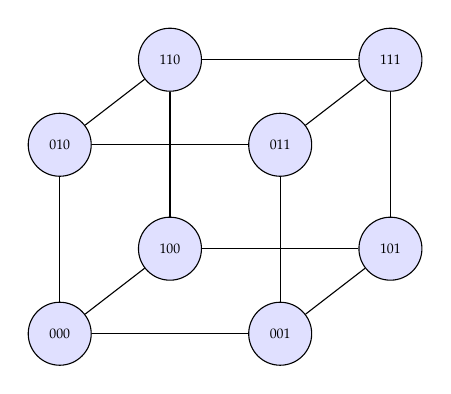
\begin{tikzpicture}[x=1.4cm,y=1.2cm]
  \node[dn,minimum size=8mm] (n000) at (0,0)     {\tiny 000};
  \node[dn,minimum size=8mm] (n001) at (2,0)     {\tiny 001};
  \node[dn,minimum size=8mm] (n011) at (2,2)     {\tiny 011};
  \node[dn,minimum size=8mm] (n010) at (0,2)     {\tiny 010};
  \node[dn,minimum size=8mm] (n100) at (1,0.9)   {\tiny 100};
  \node[dn,minimum size=8mm] (n101) at (3,0.9)   {\tiny 101};
  \node[dn,minimum size=8mm] (n111) at (3,2.9)   {\tiny 111};
  \node[dn,minimum size=8mm] (n110) at (1,2.9)   {\tiny 110};
  \begin{pgfonlayer}{background}
  \draw (n000)--(n001)--(n011)--(n010)--(n000);
  \draw (n100)--(n101)--(n111)--(n110)--(n100);
  \draw (n000)--(n100) (n001)--(n101) (n011)--(n111) (n010)--(n110);
  \end{pgfonlayer}
\end{tikzpicture}
\end{center}

\textbf{Construction and numbering.} A $d$-dimensional hypercube is built from \emph{two} $(d-1)$-dimensional hypercubes by joining each node of one to the
corresponding node of the other. If you prefix the labels of one copy with $0$ and the other with $1$, you get the numbering in the figure.

\begin{keyidea}
\textbf{Two nodes are neighbours exactly when their labels differ in one bit}, and the distance between any two nodes equals the number of
bits in which their labels differ (the \emph{Hamming distance}). Example: $0110$ and $0101$ differ in two bits, so they are two links apart.
\end{keyidea}

This gives the routing rule (\emph{e-cube routing}): to go from $a$ to $b$, look at $a\oplus b$ (bitwise exclusive-or) and flip the differing bits one at a time.
It also gives the diameter: labels have $\log_2 p$ bits, so at most $\log_2 p$ flips are needed. The cost is that each node needs $\log_2 p$ links,
which grows with machine size, and many parallel algorithms (reductions, sorting, FFT) are designed to exploit this structure.

\subsection{Trees and fat trees}

\begin{center}
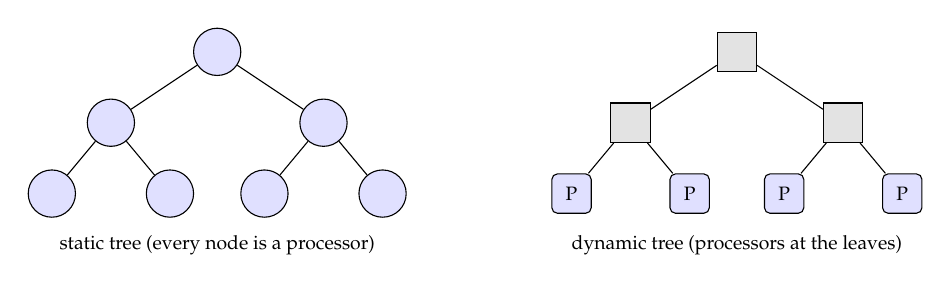
\begin{tikzpicture}[level distance=0.9cm,
   level 1/.style={sibling distance=3.2cm},level 2/.style={sibling distance=1.5cm},
   every node/.style={}]
  % static tree
  \node[dn] at (1.7,2.0) (r) {};
  \foreach \x/\p in {0.35/a,3.05/b} { \node[dn] (\p) at (\x+0.0,1.1) {}; \draw (r) -- (\p); }
  \foreach \x/\p/\q in {-0.4/c/a,1.1/d/a,2.3/e/b,3.8/f/b} { \node[dn] (\p) at (\x,0.2) {}; \draw (\q) -- (\p); }
  \node[font=\scriptsize] at (1.7,-0.45) {static tree (every node is a processor)};
  % dynamic tree
  \begin{scope}[shift={(6.6,0)}]
  \node[swt] at (1.7,2.0) (R) {};
  \foreach \x/\p in {0.35/A,3.05/B} { \node[swt] (\p) at (\x,1.1) {}; \draw (R) -- (\p); }
  \foreach \x/\p/\q in {-0.4/C/A,1.1/D/A,2.3/E/B,3.8/F/B} { \node[pe,minimum width=5mm,minimum height=5mm,font=\scriptsize] (\p) at (\x,0.2) {P}; \draw (\q) -- (\p); }
  \node[font=\scriptsize] at (1.7,-0.45) {dynamic tree (processors at the leaves)};
  \end{scope}
\end{tikzpicture}
\end{center}

A tree has exactly one path between any two nodes. In a \emph{static} tree every node is a processor; in a \emph{dynamic} tree
the inner nodes are switches and the processors are the leaves (the slide notes that ``our campus network'' is a tree).
Routing is easy: send the message \emph{up} to the lowest common ancestor of source and destination, then \emph{down}.

The weakness is the top: all messages between the left and right halves must pass through the root, which becomes the bottleneck.

\begin{definition}{fat tree}
A tree in which \emph{links get thicker towards the root}: the number of links between a node and its parent equals the number of links from that node down to its
children (the slide's ``fundamental property''). In a binary tree with one link per leaf, a switch one level above the leaves has $2$ links up, the next
level $4$, and so on.
\end{definition}

\begin{center}
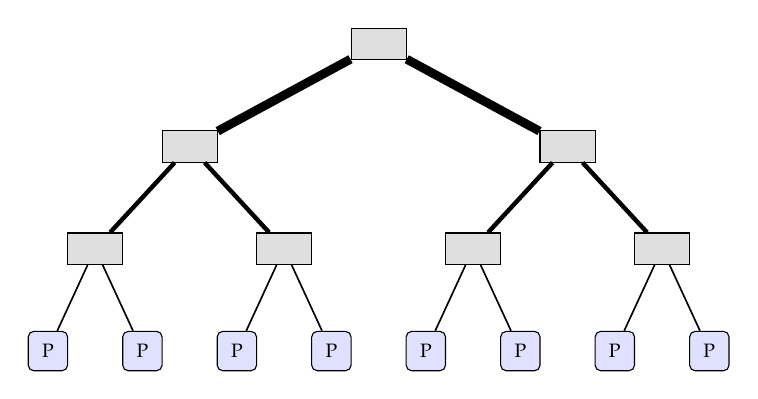
\begin{tikzpicture}[sw/.style={draw,fill=gray!25,minimum width=7mm,minimum height=4mm}]
  \foreach \i in {0,...,7} \node[pe,minimum width=5mm,minimum height=5mm,font=\scriptsize] (l\i) at (1.2*\i,0) {P};
  \foreach \i in {0,...,3} \node[sw] (a\i) at (2.4*\i+0.6,1.3) {};
  \foreach \i in {0,1} \node[sw] (b\i) at (4.8*\i+1.8,2.6) {};
  \node[sw] (c) at (4.2,3.9) {};
  \foreach \i in {0,...,3} { \draw[line width=0.6pt] (l\the\numexpr2*\i\relax) -- (a\i); \draw[line width=0.6pt] (l\the\numexpr2*\i+1\relax) -- (a\i); }
  \foreach \i/\k in {0/0,1/0,2/1,3/1} { \draw[line width=1.6pt] (a\i) -- (b\k); }
  \foreach \i in {0,1} { \draw[line width=3.2pt] (b\i) -- (c); }
\end{tikzpicture}
\end{center}

Because the capacity towards the root keeps pace with the number of processors below, \emph{any} pair of processors can communicate at full
speed without contention: a fat tree is a \emph{non-blocking} network. Its bisection width grows in proportion to $p$ (cutting at the root severs $p/2$ links' worth of
capacity), so the bisection bandwidth \emph{per node} stays constant. The slide calls these \term{constant bisection bandwidth} (CBB) networks.
A two-level fat tree has diameter $4$ (leaf, switch, root, switch, leaf: four links). In practice, thick links are built from many ordinary
links and identical small switches; most commodity clusters use a fat-tree-like network.

\section{Dynamic networks}
\slides{25--27}

\subsection{Bus}

A \term{bus} is a single set of wires shared by all attached devices. Only one transfer can take place at a time. Cost grows
linearly with the number of nodes and any two nodes are one ``hop'' apart, but the \emph{total} bandwidth is fixed, so each node's share falls as $1/p$. A bus
(or a ring, as the slide adds) is used only in small shared-memory systems. Local caches help by keeping most accesses off the bus. A bus is also what makes snooping
possible (Chapter~\ref{ch:coherence}): everything is naturally broadcast.

\subsection{Crossbar}

\begin{center}
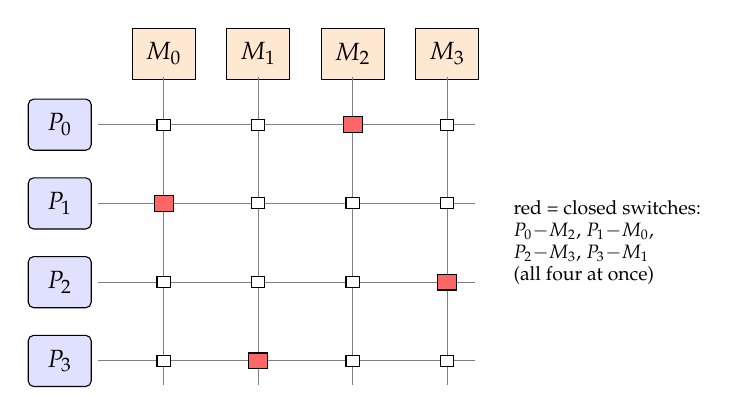
\begin{tikzpicture}[x=1.2cm,y=1.0cm]
  \foreach \i in {0,...,3} { \node[mm,minimum width=8mm] (M\i) at (\i,3.9) {$M_\i$}; \node[pe,minimum width=8mm] (P\i) at (-1.1,3-\i) {$P_\i$}; }
  \foreach \i in {0,...,3} { \draw[gray] (\i,3.6) -- (\i,-0.3); \draw[gray] (-0.7,3-\i) -- (3.3,3-\i); }
  \foreach \i in {0,...,3} \foreach \j in {0,...,3} { \draw[fill=white] (\i-0.07,3-\j-0.07) rectangle (\i+0.07,3-\j+0.07); }
  \draw[fill=red!60] (2-0.1,3-0-0.1) rectangle (2+0.1,3-0+0.1);
  \draw[fill=red!60] (0-0.1,3-1-0.1) rectangle (0+0.1,3-1+0.1);
  \draw[fill=red!60] (3-0.1,3-2-0.1) rectangle (3+0.1,3-2+0.1);
  \draw[fill=red!60] (1-0.1,3-3-0.1) rectangle (1+0.1,3-3+0.1);
  \node[font=\scriptsize,align=left,anchor=west] at (3.6,1.5) {red = closed switches:\\$P_0{-}M_2$, $P_1{-}M_0$,\\$P_2{-}M_3$, $P_3{-}M_1$\\(all four at once)};
\end{tikzpicture}
\end{center}

A \term{crossbar} connects $p$ processors to $b$ memory banks with a $p\times b$ grid of switching elements. Each crossing can
either connect or isolate its row wire and its column wire. A processor reaches any memory by closing the switch at the crossing of its row and the
memory's column.

\begin{itemize}
  \item \textbf{Non-blocking}: connecting one processor to one memory never prevents any other processor from connecting to any other \emph{free} memory. Any permutation can be realised at once, as in the figure.
  \item \textbf{Cost}: $\Theta(pb)$ switches. Usually $b\ge p$ so that every processor can find a free bank, so the cost is at least $\Omega(p^{2})$.
        This is why crossbars suit only small or medium machines (and why they are used inside switch chips): performance scales,
        \emph{cost} does not.
\end{itemize}

\subsection{Multistage networks and the Omega network}

A \term{multistage network} sits between the bus (cheap, low performance) and the crossbar (high performance, expensive): several stages of small
switches, traded for fewer switches than a crossbar and more bandwidth than a bus. The slide's example is the \term{Omega network}.

\textbf{Structure.} With $p$ inputs (processors) and $p$ outputs (memory banks), the Omega network has $\log_2 p$ \emph{stages}, each made of $p/2$
two-input, two-output switches. Each switch is in one of two settings: \emph{pass-through} (inputs go straight to the outputs) or \emph{cross-over}
(the two are swapped). The wiring between stages (and into the first stage) is the \term{perfect shuffle}: input $i$ is connected to output
\[
  j = \begin{cases} 2i & 0\le i\le p/2-1,\\ 2i+1-p & p/2\le i\le p-1,\end{cases}
\]
which is the same as rotating the binary representation of $i$ one position to the left. For $p=8$: $001\to010$, $010\to100$,
$101\to011$, and $000$, $111$ map to themselves.

\textbf{Why $\log_2 p$ stages?} Each stage can decide one bit of the destination address; with $p=2^k$ destinations you need $k$ decisions.

\textbf{Routing.} To send from source $s$ to destination $t$, both written in binary with the most significant bit first: at stage $k$ ($k=1,2,\dots$), compare the
$k$-th bit of $s$ with the $k$-th bit of $t$. If they are \emph{equal}, the switch is set to pass-through; if they \emph{differ}, to cross-over. After $\log_2 p$
stages the message arrives at $t$.

\begin{workedex}{routing in an $8\times 8$ Omega network}
Route $010\to111$: compare bit by bit: $0$ vs $1$ differ $\Rightarrow$ cross; $1$ vs $1$ same $\Rightarrow$ pass; $0$ vs $1$ differ $\Rightarrow$ cross.
Route $110\to100$: $1$ vs $1$ same $\Rightarrow$ pass; $1$ vs $0$ differ $\Rightarrow$ cross; $0$ vs $0$ same $\Rightarrow$ pass.
\end{workedex}

\begin{center}
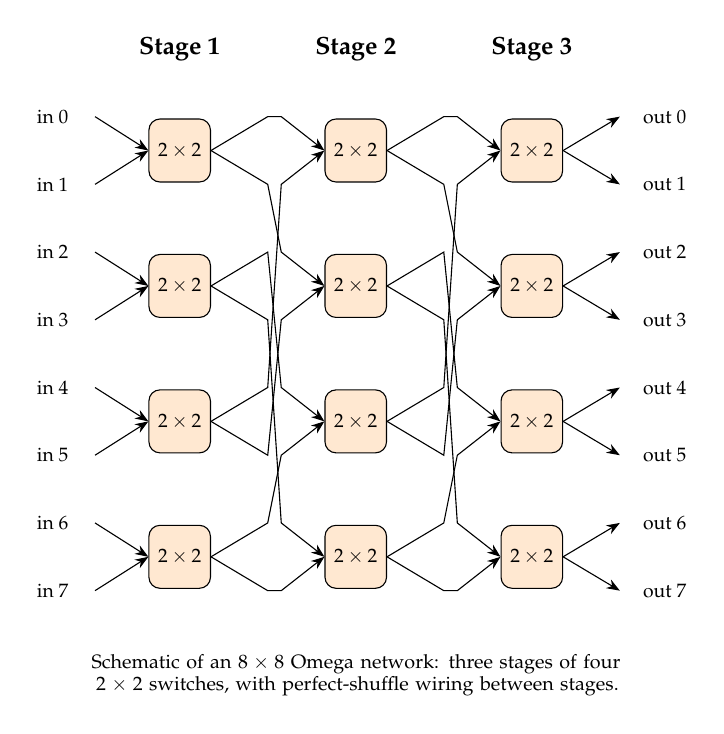
\begin{tikzpicture}[scale=0.86, every node/.style={font=\scriptsize}]
  % Illustrative 8x8 Omega network: three stages, four 2x2 switches per stage.
  \foreach \i in {0,...,7} {
    \node[left] at (0,7-\i) {in \i};
    \node[right] at (8.2,7-\i) {out \i};
  }
  \foreach \s/\x in {1/1.5,2/4.1,3/6.7} {
    \node[font=\small\bfseries] at (\x,8.0) {Stage \s};
    \foreach \j in {0,...,3} {
      \node[draw,rounded corners,fill=orange!18,minimum width=7mm,minimum height=8mm] (sw\s\j) at (\x,6.5-2*\j) {$2\times2$};
    }
  }
  % Inputs to stage 1 (paired adjacent lanes).
  \foreach \i in {0,...,7} {
    \pgfmathtruncatemacro{\j}{int(floor(\i/2))}
    \draw[->] (0.25,7-\i) -- (sw1\j.west);
  }
  % Perfect-shuffle wiring between stages: output lane i goes to input lane (2i mod 7), with 7 fixed.
  \foreach \i in {0,...,7} {
    \pgfmathtruncatemacro{\src}{int(floor(\i/2))}
    \pgfmathtruncatemacro{\k}{ifthenelse(\i==7,7,mod(2*\i,7))}
    \pgfmathtruncatemacro{\j}{int(floor(\k/2))}
    \draw[->] (sw1\src.east) -- (2.8,7-\i) -- (3.0,7-\k) -- (sw2\j.west);
  }
  \foreach \i in {0,...,7} {
    \pgfmathtruncatemacro{\src}{int(floor(\i/2))}
    \pgfmathtruncatemacro{\k}{ifthenelse(\i==7,7,mod(2*\i,7))}
    \pgfmathtruncatemacro{\j}{int(floor(\k/2))}
    \draw[->] (sw2\src.east) -- (5.4,7-\i) -- (5.6,7-\k) -- (sw3\j.west);
  }
  \foreach \i in {0,...,7} {
    \pgfmathtruncatemacro{\j}{int(floor(\i/2))}
    \draw[->] (sw3\j.east) -- (8.0,7-\i);
  }
  \node[align=center,text width=8cm] at (4.1,-1.25) {Schematic of an $8\times8$ Omega network: three stages of four $2\times2$ switches, with perfect-shuffle wiring between stages.};
\end{tikzpicture}

\end{center}

\textbf{Cost.} $\log_2 p$ stages of $p/2$ switches give $\tfrac p2\log_2 p=\Theta(p\log p)$ switches, which lies between the bus ($\Theta(p)$) and the
crossbar ($\Theta(p^{2})$). For $p=1024$: a crossbar has $1024^2=1\,048\,576$ crosspoints; an Omega network has
$512\times 10=5120$ two-by-two switches (a $2\times2$ switch is equivalent to $4$ crosspoints, so about $20\,000$). The number of stages, and hence the latency, grows only as $\log p$.

\textbf{Blocking.} Unlike the crossbar, an Omega network is a \emph{blocking} network: there is exactly \emph{one} path between each input and output, and two messages with
different sources \emph{and} different destinations can still need the same switch output.
The figure shows $010\to100$ (solid blue) and $110\to111$ (dashed red) at the same time. Both arrive at the same first-stage switch and both need its
same output, so one must wait. In the crossbar, the slide's ``non-blocking'' contrast, these two requests would both be served immediately.

\begin{workedex}{how restrictive is blocking?}
An $8\times8$ Omega network has $\tfrac p2\log_2 p=12$ switches, each with $2$ settings, so only $2^{12}=4096$ different switch settings, and each setting
realises a different permutation. But there are $8!=40\,320$ permutations of $8$ inputs onto $8$ outputs. The Omega network can realise only
about $10\%$ of them. For $p=16$ the figures are $2^{32}\approx4.3\times10^{9}$ settings against $16!\approx2.1\times10^{13}$ permutations: about $0.02\%$. (I checked the $p=8$ count by
brute force.) This is the price paid for cutting the switch count.
\end{workedex}

\section{Evaluating networks}
\slides{32--34}

How do we compare topologies? The slides use these criteria.

\begin{definition}{diameter}
The \emph{maximum} distance between any two processing nodes, where distance is the length of the shortest path in links. It bounds the worst-case number
of hops.
\end{definition}

\begin{definition}{connectivity (arc connectivity)}
The \emph{minimum number of links that must be removed} to split the network into two disconnected parts. It measures the number of alternative paths
and the fault tolerance: high connectivity is better.
\end{definition}

\begin{definition}{bisection width}
The \emph{minimum number of links that must be removed} to split the network into two \emph{equal halves}. It measures the
capacity between the two halves in the worst case.
\end{definition}

\begin{definition}{channel width, channel rate, channel bandwidth, bisection bandwidth}
\textbf{Channel width}: the number of bits that a link carries simultaneously, i.e.\ the number of physical wires in it.
\textbf{Channel rate}: the peak rate at which a single wire delivers bits.
\textbf{Channel bandwidth} $=$ channel width $\times$ channel rate.
\textbf{Bisection bandwidth} $=$ bisection width $\times$ channel bandwidth: the maximum volume of communication between the two halves of the network.
\end{definition}

Two further quantities appear in comparisons: the \textbf{degree} (links per node: it determines the hardware each node needs), and the
\textbf{cost}, measured here as the \emph{number of links}.

\subsection{Deriving the values}

\begin{itemize}
  \item \textbf{Diameter.} Completely connected: $1$. Star: $2$ (leaf, hub, leaf). Ring: the farthest node is half-way round, $\lfloor p/2\rfloor$.
        2-D mesh: corner to opposite corner is $(\sqrt p-1)+(\sqrt p-1)=2(\sqrt p-1)$. 2-D torus: wraparound means at most half-way in each
        dimension, $2\lfloor\sqrt p/2\rfloor$. Hypercube: labels have $\log_2 p$ bits, so at most $\log_2 p$ flips. Complete binary tree with $p$ nodes:
        height $\log_2\frac{p+1}{2}$, and the worst pair is two leaves in different subtrees of the root, $2\log_2\frac{p+1}{2}$.
  \item \textbf{Arc connectivity.} Linear array, tree, star: $1$ (one link failing disconnects a node). Ring: $2$. 2-D mesh without wraparound: $2$ (a corner node has only two links).
        Torus: $4$. $d$-dimensional hypercube: $d$ (every node has $d$ links and removing all of them isolates it).
  \item \textbf{Bisection width.} Ring: $2$ (cut the ring in two places). 2-D mesh: $\sqrt p$ (cut the $\sqrt p$ horizontal links crossing the middle column boundary). Torus: $2\sqrt p$ (the
        wraparound links double it). Hypercube: split by one bit; every node on one side has exactly one neighbour on the other, so $p/2$ links cross.
        Completely connected: each of the $p/2$ nodes in one half has a link to each of the $p/2$ in the other, $p^2/4$ links. Tree: $1$ (cut near the root).
  \item \textbf{Cost (links).} Linear array $p-1$; ring $p$; star $p-1$; tree $p-1$; completely connected $p(p-1)/2$; 2-D mesh $2p-2\sqrt p$; 2-D torus $2p$;
        hypercube $(p\log_2 p)/2$ (each of $p$ nodes has $\log_2 p$ links and every link is counted twice); $k$-ary $d$-cube $dp$.
\end{itemize}

\begin{pitfall}
\textbf{About the star's bisection width.} The slides and the textbook table list $1$ for the star, meaning the single link whose removal disconnects the network. If you insisted on splitting
the nodes into two exactly equal halves you would have to cut about $p/2$ links (every leaf on the side without the hub). For exams, use the course value $1$,
but know that it is a convention.
\end{pitfall}

\subsection{Summary table}
\label{sec:summarytable}

\begin{center}
\small
\renewcommand{\arraystretch}{1.3}
\begin{tabular}{@{}lcccc@{}}
\toprule
\textbf{Network} & \textbf{Diameter} & \textbf{Bisection width} & \textbf{Arc connectivity} & \textbf{Cost (links)}\\
\midrule
Completely connected & $1$ & $p^{2}/4$ & $p-1$ & $p(p-1)/2$\\
Star & $2$ & $1$ & $1$ & $p-1$\\
Ring & $\lfloor p/2\rfloor$ & $2$ & $2$ & $p$\\
Linear array & $p-1$ & $1$ & $1$ & $p-1$\\
Complete binary tree & $2\log_2\frac{p+1}{2}$ & $1$ & $1$ & $p-1$\\
2-D mesh (no wraparound) & $2(\sqrt p-1)$ & $\sqrt p$ & $2$ & $2(p-\sqrt p)$\\
2-D torus (wraparound) & $2\lfloor\sqrt p/2\rfloor$ & $2\sqrt p$ & $4$ & $2p$\\
Hypercube & $\log_2 p$ & $p/2$ & $\log_2 p$ & $(p\log_2 p)/2$\\
Wraparound $k$-ary $d$-cube & $d\lfloor k/2\rfloor$ & $2k^{d-1}$ & $2d$ & $dp$\\
\bottomrule
\end{tabular}
\end{center}

\begin{workedex}{sixty-four nodes}
\begin{center}
\small
\begin{tabular}{@{}lccccc@{}}
\toprule
 & Diameter & Bisection width & Links & Degree\\
\midrule
Ring & $32$ & $2$ & $64$ & $2$\\
$8\times8$ mesh & $14$ & $8$ & $112$ & up to $4$\\
$8\times8$ torus & $8$ & $16$ & $128$ & $4$\\
6-D hypercube & $6$ & $32$ & $192$ & $6$\\
Completely connected & $1$ & $1024$ & $2016$ & $63$\\
\bottomrule
\end{tabular}
\end{center}
The torus is a good compromise: twice the links of the ring give a $4\times$ shorter diameter and an $8\times$ larger bisection. The hypercube is
better still but needs more links per node and more total links; the completely connected network is best on every performance measure and
impractical in cost.
\end{workedex}

\begin{workedex}{bisection bandwidth in numbers}
Take the $8\times8$ torus. Suppose each link has channel width $16$ wires and each wire delivers $1$~Gbit/s. Then channel bandwidth $=16\times1=16$~Gbit/s and,
with bisection width $16$, the bisection bandwidth is $16\times16=256$~Gbit/s $=32$~GB/s.
If every one of the $32$ nodes in one half sends $1$~GB to a node in the other half, $32$~GB must cross the cut, which takes at least $32/32=1$~second whatever the algorithm. This is the
sense in which bisection bandwidth bounds the speed of communication-heavy programs.
\end{workedex}

\subsection{The blanks on the slides}

The slides leave the values for you to fill in; for reference (with $P$ nodes):
diameter -- fully connected $1$, star $2$, ring $P/2$, hypercube $\log P$;
connectivity -- linear array $1$, ring $2$, 2-D mesh $2$, 2-D mesh with wraparound $4$, $d$-dimensional hypercube $d$;
bisection width -- ring $2$, $P$-node 2-D mesh $\sqrt P$, tree $1$, star $1$, completely connected $P^2/4$, hypercube $P/2$.

\subsection{Where each network is used}

\begin{itemize}
  \item \textbf{Bus}: small shared-memory systems and inside chips (with caches to reduce traffic).
  \item \textbf{Crossbar}: small shared-memory machines and small-to-medium distributed machines; also inside the switches of larger networks.
  \item \textbf{Multistage (Omega)}: medium-sized machines needing more bandwidth than a bus at lower cost than a crossbar.
  \item \textbf{Mesh/torus}: used in several large supercomputers (for example the IBM Blue Gene series used a 3-D torus; Fujitsu's Tofu interconnect is a multi-dimensional mesh/torus), and natural for grid computations.
  \item \textbf{Fat tree}: the dominant choice in commodity clusters, because it is non-blocking and can be built from standard switches.
  \item \textbf{Hypercube}: historically important (many classic parallel algorithms assume it) but rarely built today because the degree grows with $\log p$.
\end{itemize}

\begin{keyidea}
There is no best topology. Diameter measures latency, bisection width and bandwidth measure how much traffic the network can carry, connectivity measures resilience, and links per node
measure cost. Every design trades these off.
\end{keyidea}

\section*{Exercises}
\addcontentsline{toc}{section}{Exercises}
\begin{enumerate}[label=\textbf{\thechapter.\arabic*},leftmargin=*]
  \item For $p=16$ nodes, compute the diameter, bisection width and number of links of (a) a $4\times4$ mesh and (b) a $4\times4$ torus.
  \item In a $4$-dimensional hypercube, how many hops separate nodes $1011$ and $0110$? Give a path that flips the differing bits from the lowest to the highest.
  \item In a $16\times16$ Omega network, how many stages and how many switches are there? Give the switch settings (pass or cross, by stage) for the route $0101\to1100$.
  \item A binary fat tree has $16$ processors at the leaves. How many levels of switches does it have, and what is its diameter in links?
  \item A $16\times16$ torus ($256$ nodes) has channel width $32$ wires and $2$~Gbit/s per wire. Compute the channel bandwidth and the bisection bandwidth in Gbit/s and GB/s.
  \item Explain why a bus does not ``scale'' even though its cost is only $O(p)$.
  \item Compare a 3-D torus of $4096=16^3$ nodes with a $12$-dimensional hypercube of the same size in diameter, bisection width, number of links and degree.
  \item Using the cost model, how long does a message of $m=10^{4}$ words take over $l=8$ links with store-and-forward and with cut-through ($t_s=100$, $t_h=10$, $t_w=1$)?
\end{enumerate}
\chapter{Summary, Formula Sheet and Glossary}
\label{ch:summary}

\section{The whole chapter in one picture}

\begin{center}
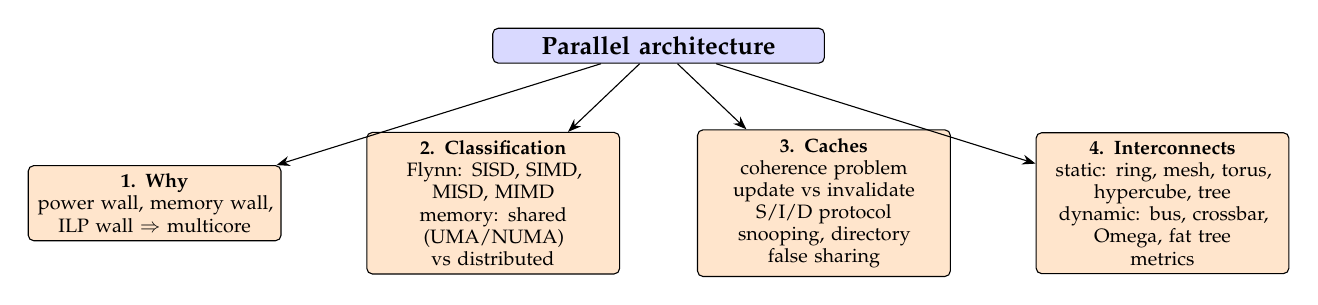
\begin{tikzpicture}[bx/.style={draw,rounded corners=2pt,fill=#1,font=\scriptsize,align=center,inner sep=3pt,text width=3.0cm}]
  \node[bx=blue!15,text width=4cm,font=\small\bfseries] (root) at (0,0) {Parallel architecture};
  \node[bx=orange!20] (a) at (-6.4,-2.0) {\textbf{1. Why}\\power wall, memory wall,\\ILP wall $\Rightarrow$ multicore};
  \node[bx=orange!20] (b) at (-2.1,-2.0) {\textbf{2. Classification}\\Flynn: SISD, SIMD, MISD, MIMD\\memory: shared (UMA/NUMA)\\vs distributed};
  \node[bx=orange!20] (c) at (2.1,-2.0)  {\textbf{3. Caches}\\coherence problem\\update vs invalidate\\S/I/D protocol\\snooping, directory\\false sharing};
  \node[bx=orange!20] (d) at (6.4,-2.0)  {\textbf{4. Interconnects}\\static: ring, mesh, torus,\\hypercube, tree\\dynamic: bus, crossbar,\\Omega, fat tree\\metrics};
  \foreach \n in {a,b,c,d} \draw[->] (root) -- (\n);
\end{tikzpicture}
\end{center}

\begin{keyidea}
Hardware designers give us parallelism because they can no longer give us speed (Chapter~1). Machines differ in what runs in parallel and in how memory is organised
(Chapter~2). Where several processors share memory, caches create the coherence problem, solved by hardware protocols that scale in different ways
(Chapter~3). The interconnect that carries all the traffic is judged by diameter, bandwidth, connectivity and cost (Chapter~4).
\end{keyidea}

\section{Formula and fact sheet}

\begin{center}
\small
\begin{tabularx}{\linewidth}{@{}l X@{}}
\toprule
\textbf{Topic} & \textbf{Fact}\\
\midrule
Dynamic power & $P\approx\alpha CV^{2}f$; with $V\propto f$: $P\propto f^{3}$\\
Amdahl bound & serial fraction $s$ $\Rightarrow$ speedup $\le 1/s$; with $n$ processors $S=1/(s+(1-s)/n)$\\
Flynn & SISD, SIMD (lock-step, same instruction), MISD (rare), MIMD (independent; SPMD is a MIMD programming style)\\
Shared memory & one address space; implicit communication; UMA (equal access times) or NUMA (local fast, remote slow)\\
Distributed memory & private memories; explicit messages (send/receive); scales furthest\\
Write policies & write-through: memory always updated; write-back: dirty bit, memory updated on eviction\\
Coherence & per location, behave as if there were one copy; writes serialised\\
Invariant (invalidate protocol) & for each line: many caches in S \emph{or} exactly one in D\\
States & I (no valid copy), S (valid, shared, clean), D (only valid copy, modified, memory stale)\\
Transitions & S$\xrightarrow{\text{write}}$D (others $\to$I); I$\xrightarrow{\text{read}}$S; I$\xrightarrow{\text{write}}$D; D$\xrightarrow{\Cread}$S; D$\xrightarrow{\Cwrite}$I; S$\xrightarrow{\Cwrite}$I\\
Snooping vs directory & broadcast on a bus (small) vs targeted messages using presence bits (large)\\
Full bit-vector directory & $P$ bits per line; overhead $=P/(\text{line size in bits})$\\
False sharing & different variables, same line; fix by private accumulators, padding, alignment, or contiguous per-thread blocks\\
Message cost & store-and-forward $t_s+l(t_h+mt_w)$; cut-through $t_s+lt_h+mt_w$\\
Hypercube & $p=2^{d}$; neighbours differ in one bit; distance $=$ Hamming distance; diameter $=d$\\
Omega network & $\log_2p$ stages of $p/2$ switches; $\tfrac p2\log_2 p$ switches; perfect-shuffle wiring; blocking; routing: equal bit $\to$ pass, different $\to$ cross\\
Crossbar & $p\times b$ crosspoints; non-blocking\\
Fat tree & non-blocking, constant bisection bandwidth per node; two-level diameter $4$\\
Network metrics & diameter, arc connectivity, bisection width, bisection bandwidth $=$ bisection width $\times$ channel bandwidth, channel bandwidth $=$ width $\times$ rate\\
\bottomrule
\end{tabularx}
\end{center}

The table of diameters, bisection widths, connectivities and costs of the static networks is in Section~\ref{sec:summarytable} (Chapter~\ref{ch:networks}).

\section{Self-test questions}

If you can answer these aloud without notes, you know this part of the course.
\begin{enumerate}
  \item Why did clock frequency stop increasing, and why does ``many slow cores'' beat ``one fast core'' for a fixed power budget?
  \item What is the difference between latency and bandwidth? Why does adding cores not automatically fix the memory wall?
  \item Give one example each of SISD, SIMD and MIMD hardware. Why is SPMD not SIMD?
  \item What does ``shared physical address space'' mean? Why is NUMA still shared memory?
  \item Why can't you send a pointer to another MPI process?
  \item Walk through the stale-data example. Why does write-through not fix it?
  \item State the three conditions of coherence. How is coherence different from consistency?
  \item Compare write-update and write-invalidate with an example where each wins.
  \item Draw the S/I/D state diagram from memory and explain each arrow in words, including what the owner does on \Cread{} and \Cwrite{}.
  \item Why does snooping not scale? How does a directory help, and what does it cost? Why is a full bit vector wasteful?
  \item What is false sharing? Give two different ways to remove it.
  \item Why is a crossbar non-blocking but expensive, and an Omega network cheaper but blocking? Route a message through an $8\times8$ Omega network.
  \item Define diameter, arc connectivity, bisection width and bisection bandwidth. Compute them for a ring, a torus and a hypercube.
\end{enumerate}

\section{How this connects to what comes next}

\begin{itemize}
  \item \textbf{Shared-memory hardware} $\leftrightarrow$ \textbf{OpenMP}: threads read and write shared data. Cache coherence, false sharing and NUMA
        placement decide how fast an OpenMP program runs.
  \item \textbf{Distributed-memory hardware} $\leftrightarrow$ \textbf{MPI}: explicit sends and receives. The network topology and
        the cost model of Chapter~4 decide how expensive messages and collective operations are.
  \item \textbf{Many-core processors (GPUs)} $\leftrightarrow$ \textbf{CUDA}: the next set of slides, where the SIMD idea of Chapter~2 returns in the form of thread groups
        executing in lock-step.
\end{itemize}

\section{Glossary}

\begin{description}[leftmargin=2.2cm,labelwidth=2cm,style=nextline,itemsep=2pt]
  \item[Address space] The set of addresses a program can use; virtual (per process) or physical (actual DRAM locations).
  \item[Arc connectivity] Minimum number of links whose removal disconnects the network.
  \item[Bandwidth] Amount of data transferred per unit time.
  \item[Bisection width / bandwidth] Minimum links to cut to split the network into equal halves; that number times channel bandwidth.
  \item[Blocking network] A network in which some pairs of simultaneous connections cannot both be made (Omega); non-blocking: crossbar, fat tree.
  \item[Cache coherence] Property that all processors see a consistent value for each memory location despite private caches.
  \item[Cache line] Unit of transfer and of coherence between memory and cache (64 bytes typically).
  \item[cc-NUMA] Cache-coherent non-uniform memory access.
  \item[Channel width / rate / bandwidth] Wires per link; bits per second per wire; their product.
  \item[Cut-through routing] Pipelined forwarding of a message; cost $t_s+lt_h+mt_w$.
  \item[Dirty (D) / Modified] The only valid copy, changed since memory was last updated.
  \item[Directory] Table recording which caches hold each line, used to send coherence messages only where needed.
  \item[Diameter] Largest shortest-path distance between two nodes.
  \item[False sharing] Different variables in one cache line causing needless coherence traffic.
  \item[Fat tree] Tree whose links get thicker towards the root; non-blocking.
  \item[Flynn's taxonomy] SISD/SIMD/MISD/MIMD classification by instruction and data streams.
  \item[Home node] Node whose memory holds a given line, and which keeps its directory entry.
  \item[Hypercube] $d$-dimensional network of $2^{d}$ nodes; neighbours differ in one label bit.
  \item[ILP] Instruction-level parallelism inside one core.
  \item[Invalid (I)] State of a line with no valid data in this cache.
  \item[Lock-step] All processing elements execute the same instruction at the same moment (SIMD).
  \item[Memory wall] Growing gap between processor speed and memory speed.
  \item[MESI / MOESI] Coherence protocols that add Exclusive (and Owned) states to MSI.
  \item[MIMD] Multiple instruction, multiple data: independent processors.
  \item[NUMA / UMA] Non-uniform / uniform memory access times in a shared-memory machine.
  \item[Omega network] Multistage network of $\log_2p$ stages with perfect-shuffle wiring.
  \item[Perfect shuffle] Wiring pattern connecting input $i$ to the left rotation of $i$'s binary representation.
  \item[Power wall] Limit on chip power and heat that stopped clock frequencies rising.
  \item[Presence bits] Directory bits recording which processors hold a copy of a line.
  \item[Routing] Choosing the path of a message through a network.
  \item[Shared (S)] State of a clean, read-only copy that other caches may also hold.
  \item[SIMD] Single instruction, multiple data.
  \item[Snooping] Cache controllers watching a shared bus to keep caches coherent.
  \item[SPMD] Single program, multiple data: one program text run by many processes with different data.
  \item[Stale] An out-of-date cached copy.
  \item[Torus] Mesh with wraparound links.
  \item[Write-back / write-through] Update memory on eviction (with a dirty bit) / on every write.
  \item[Write-invalidate / write-update] On a write, invalidate other copies / overwrite other copies.
\end{description}

\section{References for further reading}

\begin{itemize}
  \item A.~Grama, A.~Gupta, G.~Karypis, V.~Kumar, \emph{Introduction to Parallel Computing}, 2nd ed., Addison-Wesley, 2003: Chapter~2, especially
        Section~2.4 (the slides' recommended reading for networks and coherence), and the discussion of communication costs.
  \item D.~Culler, J.~P.~Singh, A.~Gupta, \emph{Parallel Computer Architecture: A Hardware/Software Approach}, Morgan Kaufmann, 1999:
        Chapter~1 (convergence of architectures), Chapter~5 (shared-memory multiprocessors: cache coherence, memory consistency, MSI and MESI),
        Chapter~7 (scalable multiprocessors), Chapter~8 (directory-based coherence).
  \item J.~Hennessy, D.~Patterson, \emph{Computer Architecture: A Quantitative Approach}: the chapters on multiprocessors and thread-level parallelism.
  \item P.~Pacheco, \emph{An Introduction to Parallel Programming}, Morgan Kaufmann, 2011: Chapter~2, a short overview of parallel hardware.
  \item B.~Barney, \emph{Introduction to Parallel Computing}, Lawrence Livermore National Laboratory tutorial (the source of the slides' figures).
  \item N.~Shah, \emph{Notes on Parallel Computing} (GitHub: \texttt{Nihar-Shah2001/Parallel\_Computing}): Chapter~1 for caches; Chapters~2--3 for another treatment of this material.
\end{itemize}
\chapter{Why Many-core? CPUs versus GPUs}
\label{ch:manycore}

\slides{2--3}

Part~I of these notes was about machines with a handful to a few hundred big, independent
processors. This second part is about a very different design: a chip with \emph{thousands} of
small, simple arithmetic units, the \term{many-core} processor. The most important example is the
\term{GPU} (Graphics Processing Unit). Almost every large machine-learning model and a large share of
the world's fastest supercomputers run on GPUs, so the architecture is worth understanding properly.

\section{From drawing pictures to general computing}

The slide says that GPUs were \emph{``primarily proposed for graphics applications''} and that
graphics \emph{``consists of stages with each stage consisting of independent computations''}.
Let us unpack this, because it explains the whole design.

To show a frame of a game, the computer must decide the colour of every pixel of the screen. A
$1920\times1080$ screen has about $2$ million pixels, and a new frame is needed $60$ times per second. The work per pixel is
a small program (find the surface visible at that pixel, work out the lighting, look up a texture,
blend colours). The key observation is:
\begin{keyidea}
The colour of one pixel does not depend on the colour of any other pixel in the same frame. Millions of
tiny, \emph{independent} jobs can therefore run at the same time, with no communication between them.
\end{keyidea}

The graphics work is organised as a \emph{pipeline} of stages: first the geometry of the scene
(triangles) is transformed into screen coordinates (one independent job per vertex), then triangles
are turned into pixels (one job per triangle), then each pixel is shaded (one job per pixel), and
finally the pixels are written into the frame buffer. Within every stage the jobs are independent;
only between stages is there an order. This is exactly the kind of workload for which you
want as many arithmetic units as possible, each doing the same small program on different data.

Engineers noticed that the same hardware could do other independent computations: multiplying
matrices, simulating physics on a grid, training neural networks. Using a graphics chip for
non-graphics work is called \term{GPGPU} (general-purpose computing on GPUs), and it is what we
study here.

\section{Two design philosophies}

\subsection{What a CPU core is built for}

The slide gives a number: a single CPU chip can have \emph{up to} about $128$ cores (this
figure grows from year to year; the point is the order of magnitude, tens to a couple of hundred). Each CPU core is a
large and sophisticated machine. In Part~I we met several of its tricks: deep pipelines,
out-of-order execution and speculation for instruction-level parallelism, and large multi-level caches
(Chapter~\ref{ch:coherence}). All of these exist for one purpose: to make \emph{one thread of instructions} finish
as quickly as possible, i.e.\ to minimise \term{latency}. The price is that most of the transistors
on a CPU core are spent on control logic and cache, not on arithmetic.

\subsection{What a GPU core is built for}

A GPU does the opposite. Its cores are \term{light-weight}: no speculation, no out-of-order machinery,
and tiny caches per core. In the space of one big CPU core one can place many simple arithmetic units.
The GPU does not try to make any \emph{one} thread fast. It tries to finish the \emph{total} work
quickly by running a huge number of threads at once, i.e.\ to maximise \term{throughput}.

\begin{definition}{latency and throughput}
\term{Latency} is the time one task takes from start to finish (seconds per task).
\term{Throughput} is the number of tasks, or the amount of work, finished per unit time (tasks per second).
They are not opposites, but a design optimised for one is usually not optimal for the other.
\end{definition}

\begin{intuition}
A sports car and a bus. The car has low latency for one passenger (it gets that person there
quickest). The bus is slow, but it moves $50$ people at once, so it has higher throughput. If you
must move $10\,000$ people from one stadium to another, you want buses. A CPU is the sports
car. A GPU is a fleet of buses.
\end{intuition}

\begin{figure}[ht]
\centering
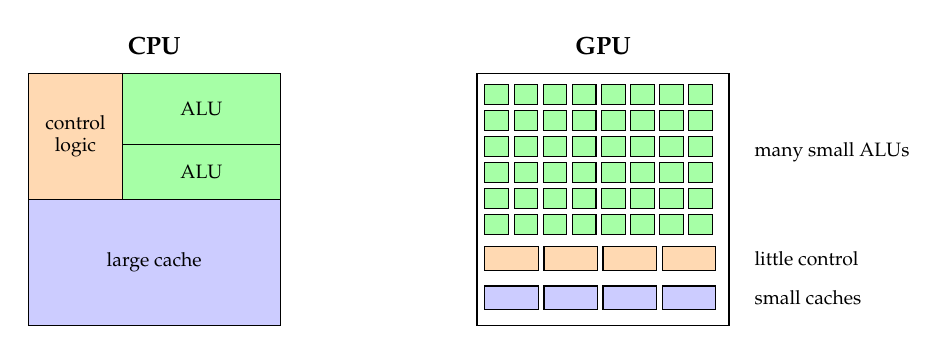
\begin{tikzpicture}[font=\scriptsize]
  % CPU
  \node at (1.6,3.55) {\small\textbf{CPU}};
  \draw (0,0) rectangle (3.2,3.2);
  \draw[fill=orange!30] (0,1.6) rectangle (1.2,3.2) node[midway,align=center] {control\\logic};
  \draw[fill=green!35] (1.2,2.3) rectangle (3.2,3.2);
  \draw[fill=green!35] (1.2,1.6) rectangle (3.2,2.3);
  \node at (2.2,2.75) {ALU};  \node at (2.2,1.95) {ALU};
  \draw[fill=blue!20] (0,0) rectangle (3.2,1.6) node[midway] {large cache};
  % GPU
  \node at (7.3,3.55) {\small\textbf{GPU}};
  \draw (5.7,0) rectangle (8.9,3.2);
  \foreach \i in {0,...,7}{\foreach \j in {0,...,5}{\draw[fill=green!35] (5.8+0.37*\i,1.15+0.33*\j) rectangle +(0.3,0.26);}}
  \foreach \i in {0,1,2,3}{\draw[fill=orange!30] (5.8+0.75*\i,0.7) rectangle +(0.68,0.3);}
  \foreach \i in {0,1,2,3}{\draw[fill=blue!20] (5.8+0.75*\i,0.2) rectangle +(0.68,0.3);}
  \node[anchor=west] at (9.1,2.2) {many small ALUs};
  \node[anchor=west] at (9.1,0.85) {little control};
  \node[anchor=west] at (9.1,0.35) {small caches};
\end{tikzpicture}
\caption{Schematic split of chip area (not to scale; an original illustration of the general idea).
A CPU spends most of its area on control logic and cache to speed up a few threads;
a GPU spends most of its area on arithmetic units.}
\label{fig:cpugpu}
\end{figure}

\begin{pitfall}
``Core'' does not mean the same thing on a CPU and a GPU. A CPU core can fetch, decode and run its own instruction stream. A
GPU ``CUDA core'' (see Chapter~\ref{ch:a100}) is just an arithmetic unit; it cannot decide
what to execute by itself. When comparing ``$128$ cores'' with ``$6912$ cores'', you are comparing
a complete processor with a single floating-point unit. Never compare these numbers directly.
\end{pitfall}

\subsection{What kind of programs suit a GPU?}

Because of its design, a GPU shines when the program has:
\begin{enumerate}
  \item \textbf{lots of data parallelism}: the same operation applied independently to many data elements
        (vector addition, matrix multiplication, image filters, neural-network layers);
  \item \textbf{high arithmetic intensity}: many arithmetic operations for every byte fetched from memory (Chapter~\ref{ch:gpumem});
  \item \textbf{regular control flow}: threads that run next to each other take the same branches (Chapter~\ref{ch:a100}).
\end{enumerate}
It performs poorly on a program that is mostly a single long chain of dependent steps (a
parser, a recursive search), because there is nothing to spread over thousands of units and the
individual GPU threads are slow.

\section{Heterogeneous computing: CPU and GPU together}

\slides{3}

The slide says that \emph{``typically GPU and CPU coexist in a heterogeneous setting''}.
\begin{definition}{heterogeneous system}
A computer that contains processors of \emph{different kinds}, here a CPU (the \term{host}) and
one or more GPUs (the \term{devices}), each used for the work it is best at.
\end{definition}

The slide's division of labour is: the ``less'' computationally intensive part runs on the CPU, and the more intensive parts run on the GPU.
It also labels these two kinds of parallelism:
\begin{itemize}
  \item \term{Coarse-grained} parallelism: a few big, long-running tasks, each doing a lot of work between synchronisations. This matches the CPU's few strong cores.
  \item \term{Fine-grained} parallelism: a very large number of tiny tasks (even one array element each). This matches the GPU's thousands of weak units.
\end{itemize}

A typical program therefore looks like this:
\begin{enumerate}
  \item The CPU runs the main program: reads input, sets things up, and does the serial parts.
  \item The CPU copies the data that the GPU needs from its own memory to the GPU's memory
        (over the PCIe bus, or NVLink).
  \item The CPU \emph{launches a kernel}, a function that runs on the GPU in many threads at once.
  \item The GPU works. Meanwhile the CPU may do other things.
  \item The CPU copies the results back and carries on.
\end{enumerate}

\begin{pitfall}
Step~2 and step~5 are not free. The GPU has its own separate memory; the CPU and GPU do not
share an address space by default (compare the distributed-memory machines of Chapter~\ref{ch:classify}!).
Moving data over the host--device link is much slower than the GPU's own memory. So a computation is only worth sending to the GPU if the speed-up it gets from the many cores is larger than the cost of the transfer.
\end{pitfall}

\begin{workedex}{is offloading worth it?}
Suppose a task needs $2$~GB of input, and the host--device link moves about $25$~GB/s (a typical PCIe~4.0 $\times16$ link: assumed numbers for illustration).
The copy takes $2/25=0.08$~s. If the CPU alone needs $0.3$~s and the GPU needs only $0.02$~s for the computation,
then the GPU path costs $0.08+0.02=0.10$~s (and the results must also be copied back), against $0.3$~s on the CPU:
still worth it. But if the CPU needed only $0.09$~s, offloading would lose, even though the
GPU kernel itself is $4.5\times$ faster than the CPU.
\end{workedex}

\section{NVIDIA and CUDA}

The slide continues: \emph{``NVIDIA's GPU architecture is called CUDA (Compute Unified Device Architecture)
architecture, accompanied by CUDA programming model, and CUDA C language''}. CUDA is therefore three things at once,
and it helps to keep them apart:
\begin{enumerate}
  \item the \textbf{hardware architecture}: how the chip is organised (Chapters~\ref{ch:a100}--\ref{ch:gpumem});
  \item the \textbf{programming model}: the way a programmer describes parallel work (grids, blocks, threads, memory spaces); this is the topic of the later CUDA lectures;
  \item the \textbf{language and tools}: CUDA~C/C++ extends C with a few keywords, and a compiler (\cl{nvcc}) builds both CPU and GPU code from one source file.
\end{enumerate}
The picture on the slide contrasts a $4$-core CPU with a $240$-core GPU of an older generation. Today's numbers are much larger
(Chapter~\ref{ch:a100}), but the ratio of ``a few strong cores'' to ``hundreds or thousands of weak ones'' is the point.

\section*{Exercises}
\begin{enumerate}[label=\textbf{\thechapter.\arabic*},leftmargin=*]
  \item In your own words, why can a graphics workload keep thousands of arithmetic units busy? Give one non-graphics example with the same property.
  \item Explain the difference between latency and throughput using a CPU thread and a GPU thread as the two examples.
  \item A colleague says ``a GPU with $6912$ cores is $54$ times better than a CPU with $128$ cores.'' Give two reasons why this comparison is not meaningful.
  \item For which of these would you expect a GPU to help a lot, and for which not? Explain briefly. (a) Adding two arrays of $10^{8}$ numbers. (b) Walking a linked list of $10^{6}$ nodes. (c) Applying a blur filter to a $4000\times3000$ image. (d) Computing the $n$-th Fibonacci number by the plain loop.
  \item The input is $4$~GB and the link bandwidth is $16$~GB/s. The results are $1$~GB. A CPU does the whole job in $1.0$~s; the GPU kernel takes $0.2$~s. Is offloading worthwhile (ignore overlap of copy and compute)? What is the speed-up?
  \item Distinguish coarse-grained from fine-grained parallelism. Which one does the GPU promote, and which one does the host CPU?
\end{enumerate}

\chapter{Inside the GPU: the NVIDIA A100}
\label{ch:a100}

\slides{4--11, 17--18}

This chapter follows the slides' tour of one real chip, the NVIDIA \textbf{A100} (``Ampere'' generation, 2020),
and its older relative the Kepler \textbf{K40}. Numbers for the A100 are checked against NVIDIA's
\emph{A100 Tensor Core GPU Architecture} whitepaper, the recommended reading in the course schedule. Where the slides and the
whitepaper differ, this is pointed out.

\section{The hierarchy of building blocks}

\slides{4--6}

A GPU is built like a company: many small units grouped into bigger and bigger groups. Reading from the top:

\begin{definition}{the GPU hierarchy (A100)}
\begin{itemize}
  \item The \term{GPU} contains several \term{Graphics Processing Clusters (GPCs)}.
  \item A GPC contains several \term{Texture Processing Clusters (TPCs)}.
  \item A TPC contains $2$ \term{Streaming Multiprocessors (SMs)}.
  \item An SM contains the actual execution units (FP32, INT32, FP64, Tensor Cores, \dots) together with its own registers and its own on-chip memory.
\end{itemize}
\end{definition}
The names are historical: ``texture'' comes from the graphics days. For computing, the only level
that really matters is the \textbf{SM}: it is the unit that is programmed and scheduled, and it is the unit
we will keep returning to.

% Schematic of the full GA100 chip (8 GPCs). A100 enables 7 GPCs / 108 SMs and 5 of the 6 HBM2 stacks.
\begin{figure}[ht]
\centering
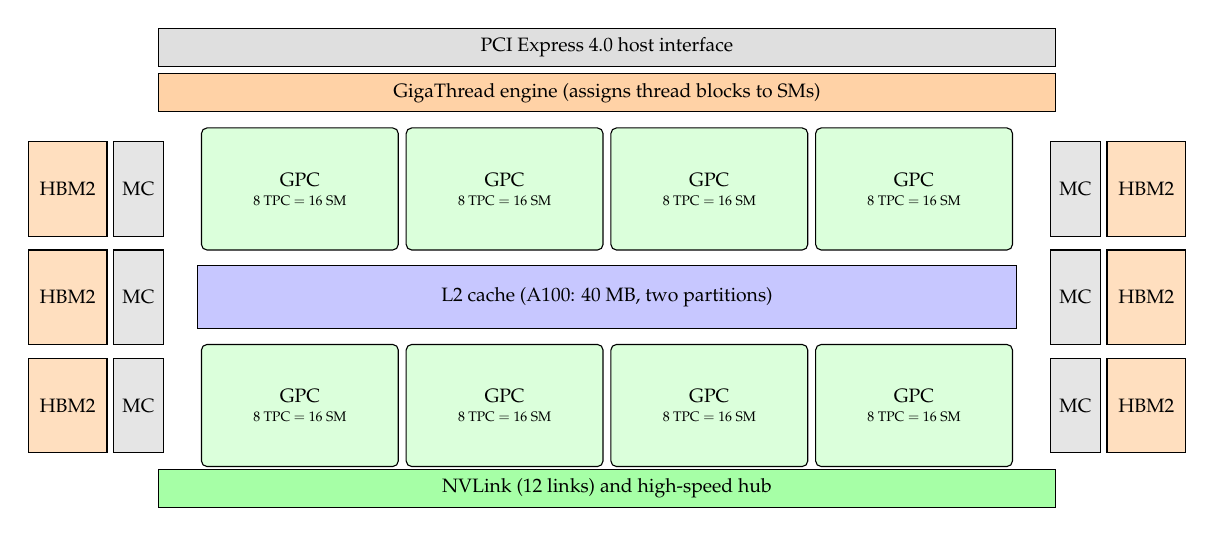
\begin{tikzpicture}[x=1cm,y=1cm,font=\scriptsize,
  gpc/.style={draw,rounded corners=2pt,fill=green!14,minimum width=2.5cm,minimum height=1.55cm,align=center},
  hbm/.style={draw,fill=orange!25,minimum width=1.0cm,minimum height=1.2cm,align=center},
  mc/.style={draw,fill=gray!20,minimum width=0.55cm,minimum height=1.2cm,align=center}]
  % top bars
  \node[draw,fill=gray!25,minimum width=11.4cm,minimum height=0.45cm] at (0,4.55) {PCI Express 4.0 host interface};
  \node[draw,fill=orange!35,minimum width=11.4cm,minimum height=0.45cm] at (0,3.97) {GigaThread engine (assigns thread blocks to SMs)};
  % GPCs top row and bottom row
  \foreach \i in {0,1,2,3}{
    \node[gpc] at (-3.9+2.6*\i,2.75) {GPC\\[-1pt]{\tiny 8 TPC $=$ 16 SM}};
    \node[gpc] at (-3.9+2.6*\i,0.0) {GPC\\[-1pt]{\tiny 8 TPC $=$ 16 SM}};
  }
  % L2
  \node[draw,fill=blue!22,minimum width=10.4cm,minimum height=0.8cm] at (0,1.375) {L2 cache (A100: 40 MB, two partitions)};
  % memory controllers and HBM left/right
  \foreach \y in {2.75,1.375,0}{
    \node[mc] at (-5.95,\y) {MC};
    \node[mc] at (5.95,\y) {MC};
    \node[hbm] at (-6.85,\y) {HBM2};
    \node[hbm] at (6.85,\y) {HBM2};
  }
  % NVLink
  \node[draw,fill=green!35,minimum width=11.4cm,minimum height=0.45cm] at (0,-1.05) {NVLink (12 links) and high-speed hub};
\end{tikzpicture}
\caption{Simplified block diagram of the full GA100 chip. The A100 product enables $7$ of the $8$ GPCs
(and not all TPCs inside them) and $5$ of the $6$ HBM2 stacks. Compare slide~5.}
\label{fig:gpu}
\end{figure}


\subsection{The numbers}

The slide says: $7$ GPCs; each GPC has $7$ or $8$ TPCs ``hence a total of $64$ TPCs''; up to $16$ SMs per GPC; ``a total of $108$ SMs''.
Table~\ref{tab:a100counts} puts the numbers together.

\begin{table}[ht]
\centering\small
\begin{tabular}{@{}lcc@{}}
\toprule
 & \textbf{Full GA100 chip} & \textbf{A100 product}\\
\midrule
GPCs & $8$ & $7$\\
TPCs per GPC & $8$ & $7$ or $8$\\
SMs per TPC & $2$ & $2$\\
SMs per GPC & $16$ & up to $16$\\
\textbf{Total SMs} & $128$ & $\mathbf{108}$\\
Total TPCs & $64$ & $54$\\
FP32 units per SM & $64$ & $64$\\
FP32 units in total & $8192$ & $6912$\\
Tensor Cores per SM & $4$ & $4$\\
Tensor Cores in total & $512$ & $432$\\
\bottomrule
\end{tabular}
\caption{The full GA100 design and the A100 product that is sold (whitepaper). Factory chips that
are ``cut down'' in this way allow dies with a few defective units to be sold.}
\label{tab:a100counts}
\end{table}

\begin{pitfall}
The slide says ``a total of $64$ TPCs'' next to ``$108$ SMs''. These two numbers do not belong
to the same chip. Since an SM pair makes a TPC, $108$ SMs means $108/2=54$ TPCs; $64$ TPCs (and $128$ SMs) is the
\emph{full} GA100 design with all $8$ GPCs. This is also why Figure~6 on slide~5 is captioned
``GA100 full GPU with $128$ SMs (A100 Tensor Core GPU has $108$ SMs)''. If a question asks for the A100, use $108$ SMs and $54$ TPCs.
\end{pitfall}

\begin{workedex}{recovering the totals}
$108$ SMs $\times$ $64$ FP32 units per SM $=6912$ FP32 units (the slide's ``$6912$ GPU cores'').
$108\times4$ Tensor Cores $=432$. The whitepaper also gives $32$ FP64 units per SM, so $108\times32=3456$ FP64 units.
Note that $7$ GPCs $\times$ $16$ SMs would give $112$; the product has only $108$ because some SMs are switched off.
\end{workedex}

\section{Inside a Streaming Multiprocessor}

\slides{7--9}

The SM is the heart of the GPU, and slide~8 is one of the most important pictures in the deck. The
slide~7 text says: each SM has $64$ FP32 cores, $4$ Tensor Cores and $192$~KB of combined shared memory and L1 data cache. Figure~\ref{fig:sm} redraws the picture.

% Schematic of one A100 SM (slides 8-9)
\begin{figure}[ht]
\centering
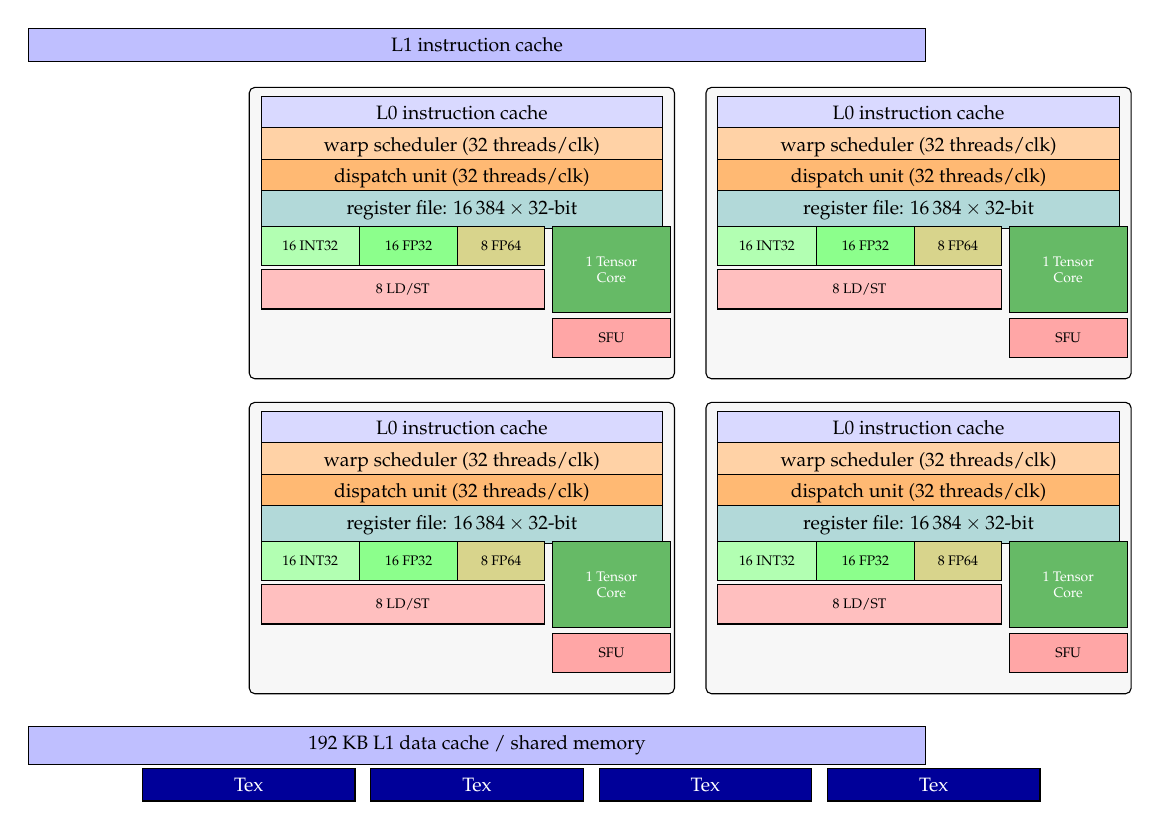
\begin{tikzpicture}[font=\scriptsize,
  part/.style={draw,rounded corners=2pt,fill=gray!6,minimum width=5.4cm,minimum height=3.7cm},
  bar/.style={draw,minimum width=5.1cm,minimum height=0.36cm,align=center},
  unit/.style={draw,minimum height=0.5cm,align=center}]
  \node[bar,fill=blue!25,minimum width=11.4cm] at (2.9,8.45) {L1 instruction cache};
  \foreach \px/\py in {0/4.2, 5.8/4.2, 0/0.2, 5.8/0.2}{
    \begin{scope}[shift={(\px,\py)}]
      \node[part,anchor=south west] at (0,0) {};
      \node[bar,fill=blue!15,anchor=north west] at (0.15,3.6) {L0 instruction cache};
      \node[bar,fill=orange!35,anchor=north west] at (0.15,3.2) {warp scheduler (32 threads/clk)};
      \node[bar,fill=orange!55,anchor=north west] at (0.15,2.8) {dispatch unit (32 threads/clk)};
      \node[bar,fill=teal!30,anchor=north west] at (0.15,2.4) {register file: $16\,384\times32$-bit};
      \node[unit,fill=green!30,minimum width=1.25cm,anchor=north west,font=\tiny] at (0.15,1.95) {16 INT32};
      \node[unit,fill=green!45,minimum width=1.25cm,anchor=north west,font=\tiny] at (1.4,1.95) {16 FP32};
      \node[unit,fill=olive!35,minimum width=1.1cm,anchor=north west,font=\tiny] at (2.65,1.95) {8 FP64};
      \node[unit,fill=green!55!black!60,minimum width=1.5cm,minimum height=1.1cm,anchor=north west,text=white,font=\tiny] at (3.85,1.95) {1 Tensor\\Core};
      \node[unit,fill=red!25,minimum width=3.6cm,anchor=north west,font=\tiny] at (0.15,1.4) {8 LD/ST};
      \node[unit,fill=red!35,minimum width=1.5cm,anchor=north west,font=\tiny] at (3.85,0.78) {SFU};
    \end{scope}
  }
  \node[bar,fill=blue!25,minimum width=11.4cm] at (2.9,-0.45) {192 KB L1 data cache / shared memory};
  \foreach \i in {0,1,2,3}{\node[bar,fill=blue!60!black,text=white,minimum width=2.7cm] at (0.0+2.9*\i-0.0,-0.95) {Tex};}
\end{tikzpicture}
\caption{One A100 SM drawn as four identical sub-partitions that share the L1/shared-memory block and the
texture units (compare slide~8). Multiplying the per-partition numbers by four gives $64$ FP32, $64$ INT32,
$32$ FP64 units, $4$ Tensor Cores and a $65\,536$-entry register file for the whole SM.}
\label{fig:sm}
\end{figure}


\subsection{Four partitions, each almost a small processor}

The SM is divided into \textbf{four identical partitions} (slide~8 shows all four; slide~9 shows two of them, enlarged). Everything with a scheduling job is replicated per partition. Each partition has:
\begin{itemize}
  \item An \textbf{L0 instruction cache} (and the SM has a shared L1 instruction cache above them), which holds the program being run.
  \item A \textbf{warp scheduler} and a \textbf{dispatch unit}, each labelled ``$32$ thread/clk'' on the slide. A \emph{warp} is a group of $32$ threads (next section); the scheduler picks a ready warp and the dispatch unit sends its next instruction to the execution units. Slide's meaning: one instruction for $32$ threads can be issued per clock per partition.
  \item A \textbf{register file} of $16\,384\times32$-bit registers ($64$~KB).
  \item The execution units: $16$ INT32 units (integer arithmetic), $16$ FP32 units (single-precision floating point), $8$ FP64 units (double precision), and $1$ Tensor Core (matrix engine, Section~\ref{sec:tensor}).
  \item $8$ load/store (LD/ST) units, which send memory requests, and a \textbf{special function unit (SFU)}, which computes things like $\sin$, $\sqrt{\ }$, $1/x$ that are too expensive for the ordinary units.
\end{itemize}
At the bottom, shared by all four partitions, sit the \textbf{$192$~KB L1 data cache / shared memory} and the \textbf{texture units} (``Tex'' on the slide, four of them).

\begin{workedex}{from one partition to the whole SM}
Per partition: $16$ FP32, $16$ INT32, $8$ FP64, $1$ Tensor Core, register file $16\,384$ entries.
Times $4$ partitions: $64$ FP32 (the slide's ``$64$ FP32 GPU cores''), $64$ INT32, $32$ FP64, $4$ Tensor Cores,
and $4\times16\,384=65\,536$ registers $=65\,536\times4$~B $=256$~KB per SM. This agrees with the whitepaper and with
the ``$64$K registers in each SMX'' on slide~14.
Over the whole chip: $108\times256$~KB $=27\,648$~KB $\approx27$~MB of registers, \emph{more than the $L2$ cache of many CPUs}.
The register file is large because each of the thousands of resident threads keeps its own variables
in it (Chapter~\ref{ch:gpumem}).
\end{workedex}

\begin{intuition}
Why does a partition with $16$ FP32 units get a scheduler that handles $32$ threads at a time? A warp has $32$ threads
but the partition has only $16$ FP32 lanes. A $32$-thread FP32 instruction therefore takes two clock cycles on that
partition's FP32 units. The scheduler is not waiting during that time, though: the A100 also has separate INT32 units, so a stream
of mixed integer and floating-point instructions from different warps can be kept running side by side.
\end{intuition}

\begin{keyidea}
An SM is \emph{not} one big core with $64$ ALUs. It is four small in-order processors, each issuing
\emph{one instruction for a whole warp} per cycle, sharing a block of fast on-chip memory.
\end{keyidea}

\section{Threads, warps and SIMT}
\label{sec:simt}

\slides{17}

Slide~17 contains the single most important phrase of the lecture: \emph{``SIMD execution (actually SIMT)''}.
The word SIMD was introduced in Chapter~\ref{ch:classify}: one instruction, many data items, executed in lock-step.
The GPU does the same but exposes it differently to the programmer.

\begin{definition}{SIMT}
\term{Single Instruction, Multiple Threads}. The programmer writes the program for \emph{one thread}, in ordinary scalar style.
The hardware runs many such threads, grouped into \term{warps} of $32$ consecutive threads. All threads of a warp are issued the same instruction in the same cycle,
each on its own data and registers, but each thread has its \emph{own} program counter state and can therefore branch independently.
\end{definition}

The hardware executes warps. The programmer thinks in threads. Compare:
\begin{center}\small
\begin{tabular}{@{}p{3.6cm}p{5.2cm}p{5.2cm}@{}}
\toprule
 & \textbf{SIMD (CPU vector unit)} & \textbf{SIMT (GPU warp)}\\
\midrule
Program written as & operations on a \emph{vector} (e.g.\ $8$ numbers per instruction) & code for a single \emph{thread}\\
Registers & one wide vector register & each thread has its own private registers\\
Branching & programmer uses masks by hand & each thread can take its own branch; hardware handles it\\
Memory access & vector load of consecutive addresses & each thread has its own address\\
\bottomrule
\end{tabular}
\end{center}

\subsection{Branch divergence}

Because the $32$ threads of a warp share one instruction stream, what happens if they disagree at an \cl{if}?
\begin{lstlisting}
if (x[i] > 0)      // some threads of the warp true, some false
    y[i] = sqrt(x[i]);
else
    y[i] = 0;
\end{lstlisting}
The hardware runs \emph{both} paths one after the other: first it executes the \cl{if} branch with the threads that said ``true'' enabled and the others switched off (masked), then the \cl{else}
branch with the opposite set enabled. Threads that are masked off simply idle.
This is \term{branch divergence}.

\begin{workedex}{cost of divergence}
Suppose the \cl{if} part takes $10$ cycles and the \cl{else} part $6$ cycles.
If all $32$ threads of the warp take the same side, the warp spends $10$ or $6$ cycles.
If the warp is split, it spends $10+6=16$ cycles, and during the first $10$ only some lanes work.
Worst case with several nested or $k$-way branches: the time is the \emph{sum} of the path times, so
utilisation can fall to $1/32$ if each of the $32$ threads takes a different path.
\end{workedex}

\begin{pitfall}
Divergence matters only \emph{within} a warp. If threads $0$--$31$ all take the \cl{if} and threads $32$--$63$ all take the \cl{else},
there is no penalty, because these are different warps and can follow different paths. So write conditions that
are constant over aligned groups of $32$ threads whenever possible, e.g.\ \cl{if (threadIdx.x / 32 == 0)} instead of \cl{if (threadIdx.x \% 2 == 0)}.
\end{pitfall}

\subsection{How the programmer's threads reach the hardware}

\slides{12}

Slide~12 (the \emph{CUDA memory spaces} picture) already shows the programmer's view that the CUDA lectures
will develop: a \term{grid} of \term{thread blocks}, each block containing threads (``Thread $(0,0)$'', ``Thread $(1,0)$'', \dots).
For the hardware you only need the following mapping:
\begin{itemize}
  \item A launch creates a grid of thread blocks. Threads of one block are always placed together on \emph{one} SM, where they can cooperate through shared memory and wait for each other at barriers.
  \item One SM may hold several blocks at once. The whitepaper lists the A100 limits: at most $1024$ threads per block, $32$ blocks, $2048$ threads (i.e.\ $64$ warps) and $255$ registers per thread on an SM.
  \item A block is cut into warps of $32$ consecutive threads: threads $0$--$31$ form warp~0, threads $32$--$63$ warp~1, etc.
  \item The chip-level scheduler (the ``GigaThread engine'' of Figure~\ref{fig:gpu}) hands blocks to SMs as they have room. Different blocks cannot be assumed to run in any particular order.
\end{itemize}

\begin{workedex}{how much work is ``in flight''?}
One SM can hold up to $2048$ threads. With $108$ SMs the A100 can have $108\times2048=221\,184$ threads resident at once,
yet it has only $6912$ FP32 units. So there are about $32$ resident threads per FP32 unit. The reason for this surplus is latency hiding (Section~\ref{sec:latency}).
\end{workedex}

\section{Tensor cores}
\label{sec:tensor}

\slides{10}

The slide gives two lines: Tensor Cores are \emph{``specialized \dots compute cores for matrix operations for AI and HPC applications''} and \emph{``perform matrix multiply and accumulate (MMA) operations''}.

\begin{definition}{matrix multiply-accumulate (MMA)}
Given small matrices $A$, $B$, $C$, the operation $D\leftarrow A\times B+C$. A Tensor Core computes a whole small block of this (for example
$16\times8$ by $8\times8$ elements) as \emph{one} hardware operation, instead of one multiply-add per instruction.
\end{definition}

Why is this useful? Matrix multiplication of two $n\times n$ matrices needs $n^{3}$ multiply-adds. Deep learning and many scientific codes are mostly matrix multiplications, so making
this one operation much faster speeds up a whole field. A Tensor Core achieves this by reading each input element once and reusing it
for many multiply-adds inside the unit, instead of fetching operands again and again for every scalar instruction (compare the reuse arguments in Chapter~\ref{ch:gpumem}).

Slide~7 states that the $4$ Tensor Cores of an SM \emph{``together deliver $1024$ FP16/FP32 operations per clock''}. This means $1024$ fused multiply-adds (FMA) per clock \emph{per SM}
(i.e.\ $256$ per Tensor Core), for the dense, non-sparse case. We can check this against the whitepaper's headline figure of $312$ TFLOPS (FP16, dense):

\begin{workedex}{checking the Tensor Core rate}
An FMA counts as $2$ floating-point operations (one multiply, one add). Boost clock: $1410$~MHz. Then
\[
 108\ \text{SMs}\times1024\ \tfrac{\text{FMA}}{\text{clk}}\times2\ \tfrac{\text{FLOP}}{\text{FMA}}\times1.41\times10^{9}\ \tfrac{\text{clk}}{\text{s}}
 \approx 3.12\times10^{14}\ \text{FLOP/s}=312\ \text{TFLOPS}.
\]
\end{workedex}

For comparison, the ordinary FP32 units:
\begin{workedex}{peak FP32 and FP64 without Tensor Cores}
FP32: $6912$ units $\times2$ FLOP (FMA) $\times1.41$~GHz $=19.5$ TFLOPS. FP64: $3456\times2\times1.41$~GHz $=9.7$ TFLOPS.
These match the whitepaper's table. So for FP16 matrix work the Tensor Cores are about $312/19.5=16$ times faster than the ordinary FP32 pipeline.
\end{workedex}

The whitepaper lists the Tensor Core peak rates for several number formats; the lower the precision, the higher the rate.
\begin{center}\small
\begin{tabular}{@{}lrr@{}}
\toprule
\textbf{Format on the Tensor Core} & \textbf{Dense peak} & \textbf{With structured sparsity}\\
\midrule
FP64 & $19.5$ TFLOPS & ---\\
TF32 & $156$ TFLOPS & $312$ TFLOPS\\
FP16 / BF16 & $312$ TFLOPS & $624$ TFLOPS\\
INT8 & $624$ TOPS & $1248$ TOPS\\
INT4 & $1248$ TOPS & $2496$ TOPS\\
\bottomrule
\end{tabular}
\end{center}
\emph{Structured sparsity} is an Ampere feature: if the weights of a neural network are pruned in a fixed pattern (two of every four values are zero), the hardware skips the zeros and doubles the rate.

\begin{pitfall}
The whitepaper's comparison table prints ``$42$'' Tensor Cores per SM for the A100. This is a typographical slip in the document: the text says four per SM, and $432$ total $/\,108$ SMs $=4$.
\end{pitfall}

\section{The older generation: Kepler K40 (SMX)}

\slides{11, 17--18}

The slides also use the \textbf{Kepler K40} (2013) as a second example. Kepler calls its multiprocessor an \textbf{SMX} (``extreme'' SM); the slides use SMX and SM
interchangeably when discussing memory, but note the hardware difference. On the slides:
\begin{itemize}
  \item GPU cores are called \textbf{streaming processors (SPs)}; they are grouped into SMXs. This grouping ``promotes coarse and fine-level parallelism'': coarse across SMXs (different blocks), fine within an SMX (threads of a block).
  \item The K40 has $15$ SMXs of $192$ SP cores each, a total of $15\times192=2880$ SP cores.
  \item Each SMX has $65\,536$ registers, $192$ SP cores, $64$ DP (double-precision) cores, $32$ special function units, $32$ load/store units and $16$ texture filtering units.
  \item The clock is $1.065$~GHz, ``light-weight'' compared with a CPU; this is typical for GPUs (the A100 boosts to $1.41$~GHz).
\end{itemize}

\begin{center}\small
\begin{tabular}{@{}lcc@{}}
\toprule
 & \textbf{Kepler K40 (slides)} & \textbf{A100 (slides + whitepaper)}\\
\midrule
Multiprocessors & $15$ SMX & $108$ SM\\
FP32 cores per multiprocessor & $192$ & $64$\\
FP32 cores in total & $2880$ & $6912$\\
Registers per multiprocessor & $64$K & $64$K\\
Double-precision units per multiprocessor & $64$ & $32$\\
Shared memory + L1 per multiprocessor & $64$~KB & $192$~KB\\
Tensor Cores & none & $4$ per SM\\
Device memory & $12$~GB & $40$~GB (slides: $80$~GB model)\\
\bottomrule
\end{tabular}
\end{center}
Observe the trend: each generation puts \emph{more, smaller} multiprocessors on the chip and more on-chip memory per multiprocessor,
while the number of registers per multiprocessor stayed the same.

\begin{intuition}
Compare Figure~\ref{fig:sm} with slide~11. The K40 SMX is one big sea of $192$ cores with four schedulers in front of them.
The A100 SM is four self-contained quarters. Splitting the unit into partitions keeps the wiring between a scheduler and its execution units short
and simple, and makes it cheaper to add features such as a Tensor Core to each quarter.
\end{intuition}

\section*{Exercises}
\begin{enumerate}[label=\textbf{\thechapter.\arabic*},leftmargin=*]
  \item List the levels of the A100 hierarchy from the GPU down to an FP32 unit, and give how many of each lower-level component sit in one higher-level component.
  \item The slide says ``a total of $64$ TPCs'' and ``a total of $108$ SMs''. Explain why both cannot be true for the A100, and give the correct number of TPCs.
  \item Starting from one SM partition ($16$ FP32, $8$ FP64, $1$ Tensor Core, $16\,384$ registers), derive the per-SM and per-chip numbers of FP32 units, FP64 units, Tensor Cores and register-file size ($108$ SMs).
  \item Compute the peak FP32 rate of the A100 in TFLOPS at $1.41$~GHz. Why do we multiply by $2$?
  \item A warp executes \cl{if (tid \% 4 == 0) A(); else B();}, where \cl{A} takes $20$ cycles and \cl{B} takes $30$. How many cycles does the warp take? What fraction of the thread-slots do useful work while \cl{A} runs? Rewrite the condition so that there is no divergence for a block of $128$ threads (keeping the same amount of work for each path).
  \item Explain SIMT and say how it differs from the SIMD vector unit of a CPU. Why is it still ``lock-step'' execution?
  \item Starting from the claim of $1024$ FMA per clock per SM, reproduce the $312$ TFLOPS figure, and then compute how many times faster the FP16 Tensor Core rate is than the FP32 CUDA-core rate.
  \item How many warps can be resident on one SM, given the limit of $2048$ threads? How many per partition if they are spread evenly?
\end{enumerate}

\chapter{GPU Memory Hierarchy}
\label{ch:gpumem}

\slides{12--15}

A GPU can do arithmetic much faster than it can fetch the numbers to do arithmetic on. Most of the effort of GPU programming goes into
feeding the units. This chapter covers the memory system as presented in the slides: the CUDA memory spaces, the hierarchy and its latencies, and the differences from CPU threads.
It then adds the explanations (latency hiding, coalescing, bank conflicts, occupancy) that the instructor gives in class and that the slides can only hint at; these
extra parts are marked \emph{beyond the slides}.

\section{The CUDA memory spaces}

\slides{12}

Slide~12 (a figure from an NVIDIA course) shows what a thread can access. Study it as a map of \emph{who can see what}:

\begin{center}\small
\renewcommand{\arraystretch}{1.25}
\begin{tabularx}{\linewidth}{@{}l l l X@{}}
\toprule
\textbf{Memory} & \textbf{Visible to} & \textbf{Access} & \textbf{Where it lives and what it is for}\\
\midrule
Registers & one thread & read/write & on the SM; fastest; a thread's scalar variables\\
Local memory & one thread & read/write & private to the thread but stored in \emph{device memory}; used when registers run out (``spills'') and for large per-thread arrays\\
Shared memory & all threads of one block & read/write & on the SM; programmer-managed scratch-pad shared by the block\\
Global memory & all threads of the grid, and the host & read/write & off-chip device DRAM (HBM2 on the A100); big and slow; persists across kernel launches\\
Constant memory & all threads, and the host & read-only for threads & device DRAM plus a small cache; for values every thread reads\\
Texture memory & all threads, and the host & read-only for threads & device DRAM plus a texture cache; good for reads with 2-D spatial locality\\
\bottomrule
\end{tabularx}
\end{center}
``The host can read/write global, constant and texture memory (stored in DRAM)'': the CPU copies data in and out of exactly these three; it cannot touch a block's shared memory or a thread's registers.

\begin{pitfall}
\emph{Local} memory sounds fast, because in a CPU ``local'' means on the stack and cached. On a GPU it is a name for \emph{scope} (private to a thread),
not a place: the data is in device DRAM, with the latency of global memory. Excessive use of registers pushes a thread's variables into local memory and slows the kernel down (see occupancy below).
\end{pitfall}

\section{Global (device) memory}

\slides{13}

\begin{definition}{global memory}
The main memory of the GPU. It can be accessed by all threads running on all the SMs, and by the CPU host. It is implemented with DRAM stacks next to the processor chip.
\end{definition}
The slide quotes $12$~GB for the Kepler K40 and $80$~GB for an A100. The A100 comes in two memory sizes; the whitepaper describes the original $40$~GB card, and an $80$~GB version was
released later with the same architecture. Both are consistent with the slide.

\paragraph{HBM2 and bandwidth (from the whitepaper).}
The A100 uses \term{HBM2} (high-bandwidth memory): DRAM chips stacked on top of each other and mounted beside the GPU on the same package, connected by a very wide bus. The $40$~GB A100 has $5$ active stacks, a $5120$-bit interface, and
data rate $1215$~MHz DDR (double data rate: two transfers per clock). Therefore
\begin{workedex}{A100 memory bandwidth}
\[
 \frac{5120\ \text{bits}}{8\ \text{bits/byte}}\times1215\times10^{6}\ \tfrac{\text{clk}}{\text{s}}\times2\ \tfrac{\text{transfers}}{\text{clk}}
 =1.555\times10^{12}\ \text{B/s}=1555\ \text{GB/s}.
\]
This equals the whitepaper's $1555$~GB/s, about $1.7\times$ the V100's $900$~GB/s. A typical desktop CPU with dual-channel DDR4 reaches only a few tens of GB/s.
\end{workedex}

Between the SMs and global memory sits a large cache that all SMs share: the \textbf{L2 cache}, $40$~MB on the A100 (whitepaper), about $7\times$ the V100's, shown in blue in Figure~\ref{fig:gpu}.
The L2 is the point of coherence for the whole GPU: the whitepaper states that it provides hardware cache coherence across the full chip, so, unlike the many private caches of Chapter~\ref{ch:coherence}, the programmer does not have to reason about stale copies of global data in L2.

\paragraph{The arithmetic-intensity gap (beyond the slides).}
\begin{workedex}{FLOPs per byte the A100 needs}
Peak FP32 is $19.5$ TFLOPS and memory delivers $1555$~GB/s, so to keep the FP32 units busy the program must do
\[
 \frac{19.5\times10^{12}\ \text{FLOP/s}}{1.555\times10^{12}\ \text{B/s}}\approx12.5\ \text{FLOP per byte},
\]
i.e.\ about $50$ floating-point operations for every $4$-byte value fetched from global memory. Vector addition $c_i=a_i+b_i$ does $1$ FLOP while moving $12$ bytes ($2$ reads, $1$ write): $0.083$ FLOP/B, far below $12.5$.
It is therefore \emph{memory-bound}: the SMs wait for data and reach only $0.083/12.5\approx0.7\%$ of the peak. To reach the peak the data brought in must be \emph{reused} many times, and that is what shared memory and registers are for.
\end{workedex}

\section{Shared memory and L1}

\slides{13}

\begin{definition}{shared memory}
A small, fast memory \emph{inside each SM}, shared by all the threads of a thread block that runs on that SM. Different blocks have separate pieces of it and cannot see each other's.
\end{definition}
The slide: on the Kepler K40, the SMX has $64$~KB that can be configured as $16$, $32$ or $48$~KB of shared memory, with the rest used as L1 cache.
On the A100 it is $192$~KB per SM: the same SRAM array is split between the L1 data cache and shared memory. (The whitepaper says
shared memory can be configured to up to $164$~KB per SM, the rest being L1.)

Unlike a hardware-managed cache, nothing enters shared memory unless a thread puts it there. This is what the slides call
``cache explicitly managed'' (Section~\ref{sec:cpuvsgpu}).

\begin{workedex}{why a scratch-pad helps: tiled matrix multiplication (beyond the slides)}
Multiplying two $N\times N$ matrices, $C=AB$, every element $c_{ij}=\sum_k a_{ik}b_{kj}$.
A simple kernel in which each thread computes one $c_{ij}$ reads $2N$ values from global memory per output element: $2N^{3}$ global reads in total.
In a tiled version, a block of $T\times T$ threads loads a $T\times T$ tile of $A$ and one of $B$ into shared memory (one element per thread), then every thread uses them $T$ times
from fast shared memory. Each global value is now read once per tile and used $T$ times, so the global traffic falls by a factor $T$ to $2N^{3}/T$.
With $T=16$ the traffic is $16\times$ smaller. The programmer must write the code that loads the tiles; no hardware does it.
\end{workedex}

\paragraph{Bank conflicts (beyond the slides).}
Shared memory is split into $32$ \term{banks}, each $4$ bytes wide, and consecutive $4$-byte words go to consecutive banks (word $w$ lives in bank $w\bmod32$). The $32$ threads of a warp can all be served in one go \emph{if they hit different banks}.
If two threads of a warp ask for different words in the same bank, the accesses are serialised (a \term{bank conflict}). If all $32$ ask for different words in one bank the access is $32$ times slower.
Reading a \cl{float} array with \cl{x[tid]} is conflict-free (thread $t$ hits bank $t$). Reading \cl{x[2*tid]} gives a $2$-way conflict: threads $t$ and $t+16$ both hit bank $2t\bmod32$. (If all threads read the \emph{same} word, it is broadcast to everyone and there is no conflict.)

\section{Registers}

\slides{14}

\begin{definition}{registers}
The fastest storage, held in each SM's register file. A thread keeps its local scalar variables in registers, and the registers are \emph{private} to a thread.
\end{definition}
Slide~14: Kepler K40 and A100 both have $64$K ($65\,536$) $32$-bit registers per SM(X); that is $256$~KB of registers, more than the $192$~KB of shared memory/L1.
Registers are not time-shared as on a CPU: a resident thread keeps its registers allocated until it finishes. This has an important consequence.

\begin{definition}{occupancy}
The ratio of the number of warps resident on an SM to the maximum the SM supports ($64$ warps, i.e.\ $2048$ threads, on the A100).
\end{definition}
\begin{workedex}{registers limit how many threads fit}
The register file holds $65\,536$ registers. If every thread needs $r$ registers, at most $\lfloor65\,536/r\rfloor$ threads are resident:
\begin{center}\small
\begin{tabular}{@{}rrrr@{}}
\toprule
$r$ (regs/thread) & max threads & warps & occupancy\\
\midrule
$32$ & $2048$ & $64$ & $100\%$\\
$64$ & $1024$ & $32$ & $50\%$\\
$128$ & $512$ & $16$ & $25\%$\\
$255$ (hardware maximum) & $257\to$ rounds to $256$ & $8$ & $12.5\%$\\
\bottomrule
\end{tabular}
\end{center}
(For the last row $65\,536/255=257.0$, but threads are scheduled in whole warps and blocks, so we take $256$.) So a kernel with $32$ registers per thread can fill an SM; a kernel that needs $128$ cannot.
The same argument applies to shared memory: a block using $48$~KB of shared memory leaves room for only $\lfloor164/48\rfloor=3$ such blocks on one SM.
\end{workedex}

\section{Constant and texture memory}

\slides{14}

The slide: constant and texture memory are \emph{accessed by all the threads}. Both are read-only from the GPU's side and live in device DRAM, but each is fronted by a special cache.
\begin{itemize}
  \item \textbf{Constant memory}: values such as coefficients and parameters that all threads read. The cache can broadcast one value to all threads of a warp in one go.
  \item \textbf{Texture memory}: ``used to improve performance of reads that exhibit spatial locality among the threads''. A texture cache is organised for $2$-D neighbourhoods: thread $(x,y)$ reading the pixel at $(x,y)$ will often be next to a thread that reads $(x+1,y)$ or $(x,y+1)$; a normal row-major cache line serves only the first.
\end{itemize}

\section{Latency numbers and latency hiding}
\label{sec:latency}

\slides{14}

The slide gives two latencies: global/device memory about $200$--$400$ clock cycles (``about $300$~ns''), and shared memory about $20$--$30$ cycles (``about $5$~ns'').
Take the \emph{cycle} counts as the information to remember: the conversion to nanoseconds depends on the clock (at $1$~GHz a cycle is $1$~ns,
so $300$ cycles is $300$~ns and $25$ cycles is $25$~ns, not $5$~ns). What matters is the ratio: global memory is roughly $10$ times slower than shared memory, and a few hundred times slower than a register access (about one cycle of dependent latency).

\paragraph{How a GPU deals with $300$-cycle latency (beyond the slides).}
A CPU core handles memory latency with big caches and speculation. A GPU has neither in large amounts. Instead the SM simply \emph{switches to another warp}.
Each partition's scheduler looks at its resident warps, and each cycle picks one that is ready (its operands have arrived). When a warp issues a load and has to wait $300$ cycles, the scheduler runs other warps in the meantime.
If enough warps are resident, some warp is always ready and the execution units never sit idle.
\begin{definition}{latency hiding}
Covering the waiting time of some threads by doing useful work for other threads, through fast thread switching and a large pool of resident threads.
\end{definition}

\begin{workedex}{how much parallelism hides the memory latency? (Little's law)}
In steady state, \emph{the amount of data that must be in flight} equals bandwidth $\times$ latency. For the A100 at $1.41$~GHz,
$300$ cycles is $300/1.41\times10^{9}\approx213$~ns, so
\[
 1555\ \text{GB/s}\times213\ \text{ns}\approx331\ \text{KB}
\]
must be outstanding at any moment to keep HBM2 busy. Over $108$ SMs this is about $3.1$~KB per SM, e.g.\ $\approx 770$ threads, each with one $4$-byte load pending.
This is only possible with thousands of resident threads. A CPU core with, say, $10$ outstanding loads could never do it, which is why ``many threads'' is not a luxury for a GPU, it is a necessity.
\end{workedex}

\paragraph{Coalescing (beyond the slides).}
When the $32$ threads of a warp execute a load, the hardware combines their addresses into as few \emph{memory transactions} as possible: global memory is served in aligned chunks (typically $32$-byte sectors, up to $128$-byte lines).
If thread $t$ reads the $4$-byte element $x[t]$ (consecutive addresses), the $32$ requests fall in one $128$-byte line: one transaction, $100\%$ of the fetched bytes are used.
If instead thread $t$ reads \cl{x[32*t]} (stride of $128$ bytes), each request is in a different line: $32$ transactions, and only $4$ of the $128$ fetched bytes ($3\%$) are used.
This is \term{coalescing}. Rule of thumb: have neighbouring threads access neighbouring addresses. It is the GPU counterpart of the spatial locality you know from CPU caches, but across the threads of a warp instead of across the iterations of a loop.

\begin{pitfall}
Consequence for data layout: an array of structures (\cl{struct\{float x,y,z;\} p[N]}) read as \cl{p[t].x} has a stride of $12$ bytes between neighbouring threads, which wastes bandwidth.
A structure of arrays (\cl{float x[N], y[N], z[N]}) read as \cl{x[t]} is coalesced.
\end{pitfall}

\section{How GPU threads differ from CPU threads}
\label{sec:cpuvsgpu}

\slides{15}

Slide~15 lists two differences from CPU threads.

\begin{enumerate}
  \item \textbf{Context switching is fast.} On a CPU, switching from one thread to another means that the operating system saves the registers of the old thread to memory and loads those of the new thread (hundreds to thousands of cycles).
        On a GPU, as the slide says, ``the state of a thread (thread block) stored in shared memory and registers stay till execution completion''. Every resident thread already has its own slice of the register file, so switching to another warp costs nothing: the scheduler just issues from a different warp
        in the next cycle. This is what makes latency hiding possible.
  \item \textbf{Cache explicitly managed.} A CPU cache is invisible to the programmer: the hardware decides what to keep. On a GPU, as the slide says, ``user's program will have to explicitly bring the frequently accessed data from the device to the shared memory''. The programmer writes the load into shared memory and decides what to keep.
        (There is an L1/L2 hardware cache as well, but the significant reuse is expected to be scheduled in software.)
\end{enumerate}

\paragraph{Hardware help for explicit staging (from the whitepaper).}
Staging data has traditionally cost registers and instructions: a load from global memory goes first into a register, and is then stored from there into shared memory. The A100 adds an \term{asynchronous copy} instruction that moves data directly from global memory
into shared memory, bypassing the register file, while the thread continues with other work; completion is signalled with hardware barrier objects. This allows loading the next tile while computing on the current one (``double buffering''). The whitepaper also describes
\emph{L2 cache residency control}, with which the program can tell the L2 to keep or evict specific data.

\begin{keyidea}
A CPU hides latency with caches and prediction, and the hardware does it for you. A GPU hides latency with thousands of threads that can be switched at no cost, and
the programmer must organise the data reuse. In return a GPU delivers far more arithmetic and memory bandwidth per chip.
\end{keyidea}

\section*{Exercises}
\begin{enumerate}[label=\textbf{\thechapter.\arabic*},leftmargin=*]
  \item For each of registers, local, shared, global, constant and texture memory, state who can read it, who can write it, and whether it is on-chip or in device DRAM.
  \item Why is ``local memory'' a misleading name? When does a thread use it?
  \item A kernel uses $40$ registers per thread and blocks of $256$ threads. How many threads, warps and blocks can be resident on one A100 SM if registers are the only limit? What is the occupancy? ($65\,536$ registers per SM; max $2048$ threads.)
  \item Compute the bandwidth of an HBM2 interface of $4096$ bits at $877.5$~MHz DDR (the V100 of the whitepaper), in GB/s.
  \item Vector addition of $n$ \cl{float}s: how many FLOPs and how many bytes of global traffic? Compute the arithmetic intensity and say whether it is compute-bound or memory-bound on the A100 ($12.5$ FLOP/B).
  \item In a tiled matrix multiplication with $T=32$ tiles, by what factor is the global-memory traffic reduced? How much shared memory per block do the two tiles of \cl{float}s use? Does a block fit in the K40's $48$~KB?
  \item A warp reads \cl{float a[...]}. Count the $128$-byte transactions for (a) \cl{a[t]}, (b) \cl{a[2*t]}, (c) \cl{a[32*t]}, $t=0..31$.
  \item Shared memory has $32$ banks of $4$ bytes. Which of \cl{s[t]}, \cl{s[t+1]}, \cl{s[2*t]}, \cl{s[32*t]}, \cl{s[0]} (all threads) are conflict-free, and how many-way is the conflict in the others?
  \item Why does a GPU need many more threads than it has execution units, whereas a CPU does not? Use Little's law in your answer.
  \item List the two differences between GPU and CPU threads on slide~15 and explain how each one affects the way you write a program.
\end{enumerate}

\chapter{Many-core Summary, Formula Sheet and Glossary}
\label{ch:mcsummary}

\section{The part in one picture}

\begin{center}
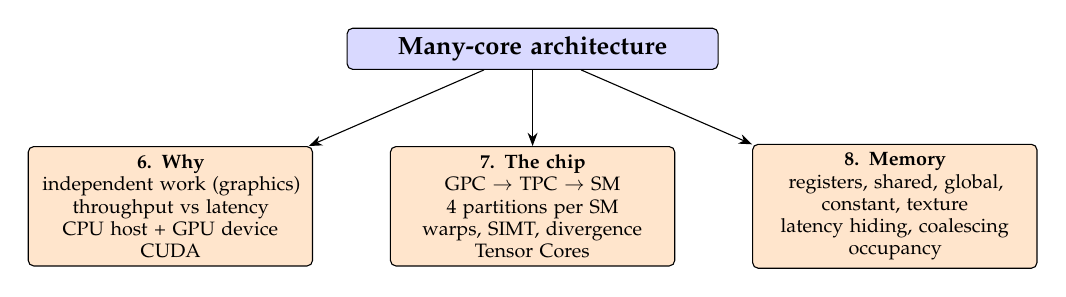
\begin{tikzpicture}[bx/.style={draw,rounded corners=2pt,fill=#1,font=\scriptsize,align=center,inner sep=3pt,text width=3.4cm}]
  \node[bx=blue!15,text width=4.5cm,font=\small\bfseries] (root) at (0,0) {Many-core architecture};
  \node[bx=orange!20] (a) at (-4.6,-2.0) {\textbf{6. Why}\\independent work (graphics)\\throughput vs latency\\CPU host + GPU device\\CUDA};
  \node[bx=orange!20] (b) at (0,-2.0) {\textbf{7. The chip}\\GPC $\to$ TPC $\to$ SM\\4 partitions per SM\\warps, SIMT, divergence\\Tensor Cores};
  \node[bx=orange!20] (c) at (4.6,-2.0) {\textbf{8. Memory}\\registers, shared, global,\\constant, texture\\latency hiding, coalescing\\occupancy};
  \foreach \n in {a,b,c} \draw[->] (root) -- (\n);
\end{tikzpicture}
\end{center}

\begin{keyidea}
A GPU gets its speed from \emph{width}, not from the speed of one thread: thousands of simple units, fed by
a huge number of cheaply-switched threads, with a fast but small on-chip memory that the programmer manages. The cost is that
the program must expose a great deal of regular data parallelism, and must reuse data on chip.
\end{keyidea}

\section{Fact and formula sheet}

\begin{center}
\small
\begin{tabularx}{\linewidth}{@{}l X@{}}
\toprule
\textbf{Topic} & \textbf{Fact}\\
\midrule
Hierarchy & GPU $\supset$ GPCs $\supset$ TPCs $\supset$ SMs ($2$ per TPC) $\supset$ $4$ partitions\\
A100 product & $7$ GPCs, $54$ TPCs, $108$ SMs; full GA100: $8$ GPCs, $64$ TPCs, $128$ SMs\\
Per SM (A100) & $64$ FP32, $64$ INT32, $32$ FP64, $4$ Tensor Cores, $65\,536$ registers ($256$~KB), $192$~KB L1/shared\\
Per chip (A100) & $6912$ FP32 cores, $3456$ FP64, $432$ Tensor Cores, $40$~MB L2, $40$ (or $80$)~GB HBM2\\
Warp & $32$ threads executed in lock-step; one scheduler per partition issues one warp-instruction per clock\\
SM limits (A100) & $2048$ threads ($64$ warps), $32$ blocks, $1024$ threads per block, $255$ registers per thread\\
Peak rate & $\text{units}\times2\times f$ ($2$ for fused multiply-add): FP32 $=6912\times2\times1.41\text{ GHz}=19.5$ TFLOPS\\
Tensor Core rate & $1024$ FMA/clk/SM; $108\times1024\times2\times1.41\text{ GHz}=312$ TFLOPS (FP16, dense)\\
HBM2 bandwidth & $\tfrac{\text{width}}{8}\times\text{clock}\times2=\tfrac{5120}{8}\times1215\text{ MHz}\times2=1555$ GB/s\\
Machine balance & peak FLOP/s $\div$ bandwidth $=19.5/1.555\approx12.5$ FLOP/B\\
Occupancy & resident warps $\div$ $64$; limited by registers: threads $\le65\,536/r$\\
Latencies & global $\approx200$--$400$ cycles; shared $\approx20$--$30$ cycles\\
Little's law & data in flight $=$ bandwidth $\times$ latency\\
Divergence & warp time $=$ sum of the times of the paths taken by its threads\\
Coalescing & consecutive threads $\to$ consecutive addresses: $1$ transaction per $128$~B; stride $\Rightarrow$ up to $32$\\
Bank conflicts & $32$ banks $\times4$~B; conflict if two threads of a warp use different words of one bank\\
Kepler K40 & $15$ SMX $\times192$ SP $=2880$ cores, $65\,536$ registers, $64$~KB shared/L1 (split $16/32/48$)\\
\bottomrule
\end{tabularx}
\end{center}

\section{Self-test questions}

\begin{enumerate}
  \item Why did graphics lead to a design with thousands of weak cores? What is the difference between a latency-oriented and a throughput-oriented chip?
  \item What runs on the host, what on the device, and what are the costs of moving between them?
  \item Draw the hierarchy of the A100 with the numbers at each level, and explain the $64$-versus-$54$ TPC inconsistency on the slides.
  \item Draw one SM and label the four partitions and their contents. Which parts are shared by the partitions?
  \item What is a warp? What is SIMT, and how does it differ from SIMD? What is branch divergence and when does it cost?
  \item What is a Tensor Core? Derive the $312$ TFLOPS figure.
  \item List the CUDA memory spaces with scope and access rights. Where is each physically?
  \item Why can a kernel run out of registers, and what does that do to occupancy?
  \item How does a GPU hide a $300$-cycle memory latency? How many bytes must be in flight to saturate the A100's HBM2?
  \item What is coalescing? What is a bank conflict? Give an access pattern for each.
  \item Name the two differences between GPU threads and CPU threads from slide~15 and what they imply for programming.
\end{enumerate}

\section{How this connects to what comes next}

\begin{itemize}
  \item \textbf{CUDA programming}: grids, blocks and threads are the programmer's names for what Chapters~\ref{ch:a100}--\ref{ch:gpumem} showed in hardware. Block size, shared-memory use and register use decide occupancy.
  \item \textbf{Parallelisation principles}: the idea of exposing enough independent work and reusing data (locality) carries over from CPUs to GPUs.
  \item \textbf{PRAM and parallel algorithms}: the SIMT model with a grid of threads and a shared memory is the nearest real machine to the PRAM model.
\end{itemize}

\section{Glossary}

\begin{description}[leftmargin=2.2cm,labelwidth=2cm,style=nextline,itemsep=2pt]
  \item[Arithmetic intensity] FLOPs performed per byte moved from memory.
  \item[Bank conflict] Two threads of a warp using different words in the same shared-memory bank; the accesses are serialised.
  \item[Branch divergence] Threads of one warp taking different paths at a branch; the paths are executed one after the other.
  \item[Coalescing] Combining the memory accesses of a warp into few transactions.
  \item[CUDA] NVIDIA's architecture, programming model and C-based language for GPUs.
  \item[Device / host] The GPU and its memory / the CPU and its memory.
  \item[FMA] Fused multiply-add, $a\leftarrow a+b\cdot c$; counts as two FLOPs.
  \item[Global memory] Off-chip device DRAM visible to all threads and the host.
  \item[GPC / TPC] Graphics Processing Cluster / Texture Processing Cluster: groups of SMs (a TPC has two).
  \item[HBM2] High-bandwidth memory: stacked DRAM next to the GPU on one package.
  \item[Heterogeneous] Containing different kinds of processors (CPU + GPU).
  \item[Kernel] A function executed on the GPU by many threads.
  \item[Latency hiding] Keeping the units busy with other threads while some threads wait for memory.
  \item[Local memory] Per-thread private memory that physically lives in device DRAM (register spills, big arrays).
  \item[MMA] Matrix multiply-accumulate, $D=AB+C$, the Tensor Core operation.
  \item[Occupancy] Resident warps divided by the maximum number of warps per SM.
  \item[SFU] Special function unit ($\sin$, $\sqrt{\ }$, reciprocal, \dots).
  \item[Shared memory] On-chip scratch-pad shared by the threads of a block.
  \item[SIMT] Single instruction, multiple threads: warp-wise lock-step execution of scalar-style thread code.
  \item[SM / SMX] Streaming multiprocessor (SMX in the Kepler generation).
  \item[SP] Streaming processor: an older name for a GPU core.
  \item[Tensor Core] Matrix-multiply unit of the SM.
  \item[Thread block] Group of threads scheduled together on one SM, sharing shared memory.
  \item[Warp] Group of $32$ threads executed together.
\end{description}

\section{References for further reading}

\begin{itemize}
  \item NVIDIA, \emph{NVIDIA A100 Tensor Core GPU Architecture} whitepaper (2020): the reading recommended in the course; numbers in this part are taken from it.
  \item D.~Kirk, W.-m.~Hwu, \emph{Programming Massively Parallel Processors}: a textbook on GPU architecture and CUDA programming.
  \item NVIDIA, \emph{CUDA C++ Programming Guide}: the authoritative description of the programming model, memory spaces, coalescing and bank rules.
  \item The figures on slides 5--6, 8--9 and 11 are from NVIDIA's whitepapers; slide~12 is from an NVIDIA CUDA course. The diagrams in these notes are original.
\end{itemize}

\chapter{Beyond the Syllabus: More on the A100}
\label{ch:beyond}

\begin{outofsyllabus}
\textbf{This whole chapter is out of syllabus.} None of it is on the Many-core Architectures slides, and I do not know whether the instructor will mention
any of it. It is here for depth, taken from NVIDIA's \emph{A100 Tensor Core GPU Architecture} whitepaper. If you only want to prepare for the course, skip it and use Chapters~6--9.
Each section below is tagged \textsc{Out of syllabus}. Numbers are from the whitepaper unless a line says ``derived'' (computed by us from the whitepaper's numbers) or ``general knowledge''.
\end{outofsyllabus}

\section{Three generations side by side}
\oos

Table~\ref{tab:gen} is the whitepaper's comparison of the A100 with its two predecessors, P100 (Pascal, 2016) and V100 (Volta, 2017).

\begin{table}[ht]
\centering\small
\begin{tabular}{@{}lrrr@{}}
\toprule
 & \textbf{P100} & \textbf{V100} & \textbf{A100}\\
\midrule
SMs & 56 & 80 & 108\\
FP32 cores / SM & 64 & 64 & 64\\
FP32 cores / GPU & 3584 & 5120 & 6912\\
FP64 cores / GPU (non-Tensor) & 1792 & 2560 & 3456\\
Tensor Cores / SM & --- & 8 & 4\\
Tensor Cores / GPU & --- & 640 & 432\\
Boost clock (MHz) & 1480 & 1530 & 1410\\
Peak FP32 (TFLOPS, non-Tensor) & 10.6 & 15.7 & 19.5\\
Peak FP64 (TFLOPS, non-Tensor) & 5.3 & 7.8 & 9.7\\
Peak FP16 Tensor (TFLOPS) & --- & 125 & 312 (624 sparse)\\
Memory interface & 4096-bit HBM2 & 4096-bit HBM2 & 5120-bit HBM2\\
Memory size & 16 GB & 32/16 GB & 40 GB\\
Memory bandwidth (GB/s) & 720 & 900 & 1555\\
L2 cache (KB) & 4096 & 6144 & 40\,960\\
Shared memory / SM (KB) & 64 & up to 96 & up to 164\\
Register file / SM (KB) & 256 & 256 & 256\\
TDP (W) & 300 & 300 & 400\\
Transistors (billions) & 15.3 & 21.1 & 54.2\\
Process & 16\,nm & 12\,nm & 7\,nm\\
\bottomrule
\end{tabular}
\caption{P100, V100 and A100 (whitepaper, Table~4).}
\label{tab:gen}
\end{table}

\begin{workedex}{what changed most from V100 to A100? (derived)}
Ratios A100/V100: SMs $108/80=1.35$; FP32 TFLOPS $19.5/15.7=1.24$; memory bandwidth $1555/900=1.73$; L2 $40\,960/6144=6.7$;
FP16 Tensor $312/125=2.5$. So the biggest jumps are the matrix engines and the L2 cache, while ordinary FP32 arithmetic grew only about $24\%$. The A100 designers
spent the new transistors (and extra $100$~W) mainly on Tensor Cores, cache and memory bandwidth, not on more general-purpose cores.
Interesting detail: the number of Tensor Cores per SM \emph{fell} from $8$ to $4$, yet the rate per SM more than doubled
(each A100 Tensor Core is $4\times$ as wide as a V100 one, see below).
\end{workedex}

\section{Third-generation Tensor Cores}
\oos

Chapter~\ref{ch:a100} introduced the Tensor Core as a matrix-multiply-accumulate engine. Here is what the whitepaper adds.

\subsection{New number formats}

Besides the FP16, INT8, INT4 and binary formats of earlier GPUs, the A100 Tensor Core supports \textbf{TF32, BF16 and FP64}.
These formats differ in how the $16$ to $64$ bits are split into a sign, an \emph{exponent} (which sets the \emph{range} of numbers) and a \emph{mantissa} (which sets the \emph{precision}).
(The bit splits below are general knowledge, not quoted from the whitepaper.)

\begin{center}\small
\begin{tabular}{@{}lccc@{}}
\toprule
\textbf{Format} & \textbf{Exponent bits} & \textbf{Mantissa bits} & \textbf{Remark}\\
\midrule
FP32 & 8 & 23 & usual ``float''\\
TF32 & 8 & 10 & FP32's range, FP16's precision; stored in a 32-bit word\\
FP16 & 5 & 10 & small range; can overflow in training\\
BF16 & 8 & 7 & FP32's range, low precision\\
\bottomrule
\end{tabular}
\end{center}
\begin{intuition}
Deep-learning training needs a wide \emph{range} more than high \emph{precision}. TF32 and BF16 keep FP32's $8$ exponent bits, so values do not overflow, and give up mantissa bits to save area and bandwidth.
A programmer can keep ordinary FP32 data in memory and let the Tensor Core round it to TF32 for the multiplication, accumulating in FP32.
\end{intuition}

The whitepaper's rate comparison (A100 versus V100, peak, per GPU):
\begin{center}\small
\begin{tabular}{@{}lrrr@{}}
\toprule
\textbf{Mode} & \textbf{V100} & \textbf{A100 dense} & \textbf{A100 sparse}\\
\midrule
FP16 Tensor & 125 TFLOPS & 312 (2.5$\times$) & 624 (5$\times$)\\
TF32 Tensor (vs.\ V100 FP32) & 15.7 TFLOPS & 156 (10$\times$) & 312 (20$\times$)\\
BF16 Tensor & --- & 312 & 624\\
FP64 Tensor & 7.8 TFLOPS & 19.5 (2.5$\times$) & ---\\
INT8 Tensor & 62 TOPS & 624 (10$\times$) & 1248\\
\bottomrule
\end{tabular}
\end{center}

\begin{workedex}{per-clock rates (derived and checked)}
The whitepaper: a V100 Tensor Core does $64$ FP16/FP32 FMAs per clock, an A100 Tensor Core $256$. Per SM: V100 $8\times64=512$; A100 $4\times256=1024$ FMA/clock, \emph{twice} the V100's per SM.
Chip peak for A100: $108\times1024\times2\times1.41$~GHz $=312$ TFLOPS, and for V100: $80\times512\times2\times1.53$~GHz $=125$ TFLOPS, matching the table.
FP64 on Tensor Cores: the whitepaper gives $64$ FP64 FMA per SM per clock, so $108\times64\times2\times1.41$~GHz $=19.5$ TFLOPS, matching the table.
This is double the $9.7$ TFLOPS of the ordinary FP64 units.
\end{workedex}

\subsection{Why the new Tensor Core also saves instructions}

On Volta, the data of one matrix operation was shared among $8$ threads of a warp; on the A100 it is shared across \textbf{all $32$ threads of the warp}, and a single instruction can cover a deeper slice of the
multiplication (up to $4\times$ larger $k$ dimension, where $k$ is the length of the dot products). The whitepaper reports for a $16\times16\times16$ multiply (per SM partition): register-file reads fall from $80$ to $28$, and
the number of issued instructions from $16$ to $2$. Fewer instructions and fewer register reads mean less power and leave the issue slots free for other work.

\section{Fine-grained structured sparsity}
\oos

Trained neural networks contain many weights that are close to zero and can be set to exactly zero with little loss of accuracy (\emph{pruning}). The A100 supports a specific pattern:
\begin{definition}{2:4 structured sparsity}
In every group of four consecutive weights, \emph{at most two are non-zero}. The two zeros per group need not be stored, so the matrix can be compressed to about half its size (plus a little index information
saying which positions were kept). The Tensor Core then multiplies only the kept values.
\end{definition}
Effect (whitepaper): storage and bandwidth cut by ``almost $2\times$'', and the Tensor Core operation takes half the cycles ($N/2$ instead of $N$ in the example), hence the factor-$2$ rows in the table above ($312\to624$ TFLOPS).
Why ``almost''? Because of the index information. Why a fixed pattern? Because a fixed pattern is easy for the hardware to decode: with random sparsity the hardware could not keep all units busy.

\begin{workedex}{a 2:4 group}
Weights $(0.8,\ 0.05,\ -0.6,\ 0.01)$: keep the two largest magnitudes $0.8$ and $-0.6$, zero the other two $\to(0.8,0,-0.6,0)$. Stored: $(0.8,-0.6)$ plus the positions ($0$ and $2$). A dense $4$-element dot product (4 multiplications) becomes $2$ multiplications.
\end{workedex}
The recommended workflow is: train the dense network, prune to the $2:4$ pattern, then \emph{fine-tune} the remaining weights to recover accuracy.

\section{More details of the SM and the memory system}
\oos

\subsection{FP32 and INT32 side by side}
The SM has separate FP32 and INT32 units, so floating-point and integer instructions can run simultaneously at full rate. The whitepaper's example is pointer and index arithmetic in loops: while an
FP32 multiply-add works on data, the INT32 units compute the address of the next element.
(This is why the SM diagram has both INT32 and FP32 columns; see Figure~\ref{fig:sm}.)

\subsection{The L2 cache in more detail}
\begin{itemize}
  \item The $40$~MB L2 is divided into \textbf{two partitions}; each partition holds data for the GPCs directly connected to it, which reduces the distance and the contention (compare the two blue halves in Figure~\ref{fig:gpu}).
  \item Each partition has $40$ slices, so $80$ slices in all; each slice is $512$~KB: $80\times512$~KB $=40$~MB (derived check). The full chip has $12$ memory controllers, the A100 has $10$, each with eight slices attached: $10\times8=80$.
  \item L2 read bandwidth is $5120$ bytes per clock (V100: $2048$): $2.5\times$. If the L2 ran at the boost clock, which the whitepaper does not state, that would be about $5120\times1.41$~GHz $\approx7.2$~TB/s, roughly $4.6\times$ the HBM2 bandwidth. The point is that data that hits in L2 is far cheaper than data from HBM.
  \item \textbf{Compute data compression}: the memory system can store data in compressed form (useful for sparse or repetitive data) and gives up to $4\times$ DRAM read/write bandwidth, up to $4\times$ L2 read bandwidth and up to $2\times$ L2 capacity.
  \item \textbf{L2 residency control}: the program can tell the hardware which data to keep in L2. A part of the cache can be set aside for \emph{persistent} accesses, in steps of $1/16$ of the cache ($40/16=2.5$~MB). The programmer marks an address range as ``persisting''; other accesses stream through the rest. The whitepaper's histogram example gets a $2.5\times$ speed-up over V100 and $43\%$ over an A100 without the control. It is not available in MIG mode.
\end{itemize}

\subsection{Asynchronous copy, asynchronous barriers}
Recall the explicit staging of Chapter~\ref{ch:gpumem}. The A100 helps in two ways:
\begin{itemize}
  \item \textbf{Asynchronous copy} (CUDA 11): data goes from global memory straight into shared memory, skipping the register file. Variants: \emph{BYPASS} (skip L1 too) and \emph{ACCESS} (also keep a copy in L1 for reuse). The thread does not wait; it issues the copy and does other work.
  \item \textbf{Asynchronous barriers}: hardware barriers in shared memory with separate \emph{arrive} and \emph{wait} operations, so a thread can say ``I'm done'' and continue with independent work before waiting. They can synchronise any subset of the threads of a block, not just whole blocks.
\end{itemize}
\begin{workedex}{what overlap buys (derived, simple model)}
Process $n$ tiles. Loading one tile takes $L$, computing on it takes $C$. Without overlap: $n(L+C)$. With double buffering (load tile $i+1$ while computing on tile $i$): about $L+(n-1)\max(L,C)+C$.
For $L=C=1$ and $n=10$: $20$ versus $1+9+1=11$ time units, nearly $2\times$ faster. If the loads go through registers they occupy registers and instruction slots; the asynchronous copy avoids both.
\end{workedex}

\subsection{Other CUDA-level improvements}
\begin{itemize}
  \item \textbf{Warp-wide reductions}: reducing $32$ values (sum, min, max, and, or, xor) used to take $\log_2 32=5$ shuffle-and-add steps; the A100 has a hardware instruction that does it in one step (reached through Cooperative Groups).
  \item \textbf{Atomic operations}: FP16 atomics are $11\times$ and FP32 atomics $2.7\times$ faster than on V100.
  \item \textbf{CUDA task graphs}: describe a whole workflow of kernels and copies as a graph once, launch it many times with one call; this cuts launch overhead for workloads of many small kernels. Cooperative launches reduced grid-synchronisation overhead by up to $30\%$.
\end{itemize}

\section{Multi-Instance GPU (MIG)}
\oos

\begin{definition}{MIG}
\term{Multi-Instance GPU} lets one A100 be divided in hardware into up to \textbf{seven} independent \term{GPU Instances}, each behaving like a smaller GPU with its own SMs, its own L2 slices, and its own part of the memory.
\end{definition}
\begin{intuition}
A big GPU is often not fully used by a small job (say, inference for one model). With MIG, one A100 serves seven such jobs at once, and a misbehaving job cannot slow down or crash the others,
because each instance has its own separate path through crossbar, L2 banks, memory controllers and DRAM address buses.
\end{intuition}
Key facts (whitepaper):
\begin{itemize}
  \item One \textbf{GPU slice} $=$ one GPC $+$ a group of $10$ L2 slices $+$ a share of the memory. In MIG mode each GPC has $7$ TPCs ($14$ SMs) enabled.
  \item A \textbf{GPU Instance} contains one or more slices. Inside it, \textbf{Compute Instances} subdivide the compute resources (by default one per GPU instance).
  \item Derived: $7$ slices $\times14$ SMs $=98$ SMs usable in MIG mode (out of $108$), and $7\times10=70$ of the $80$ L2 slices.
  \item Use cases: renting separate slices to different cloud customers; isolating the faults of different applications of one user; sharing a GPU among several users in a lab. A DGX~A100 (eight GPUs) then offers up to $8\times7=56$ separate accelerators.
  \item Limits: MIG is for compute only (no graphics), and the L2 set-aside of the previous section is disabled in MIG mode.
\end{itemize}

\section{Connecting GPUs: NVLink and PCIe}
\oos

Chapter~\ref{ch:manycore} stressed that the host--device link is slow compared with on-card memory. The whitepaper describes the two links of the A100.

\begin{center}\small
\begin{tabular}{@{}lrr@{}}
\toprule
 & \textbf{V100 NVLink~2} & \textbf{A100 NVLink~3}\\
\midrule
Signal rate per pair & 25.78 Gbit/s & 50 Gbit/s\\
Pairs per direction per link & 8 & 4\\
Bandwidth per link per direction & 25 GB/s & 25 GB/s\\
Links per GPU & 6 & 12\\
Total (both directions) & 300 GB/s & 600 GB/s\\
\bottomrule
\end{tabular}
\end{center}
\begin{workedex}{checking the NVLink numbers (derived)}
A100 link: $4$ pairs $\times50$~Gbit/s $=200$~Gbit/s $=25$~GB/s per direction. $12$ links $\times25$~GB/s $=300$~GB/s per direction, $600$~GB/s in both directions together. V100: $6\times25=150$ per direction, $300$ total.
So A100 doubles the bandwidth by doubling the \emph{number} of links, with each link having half the wires but twice the signalling rate.
\end{workedex}
\textbf{PCIe Gen~4} (host link): $31.5$~GB/s per direction for an $\times16$ slot, twice PCIe~3. Compare with NVLink's $300$~GB/s per direction: about $9.5\times$ (derived).
In the offload example of Chapter~\ref{ch:manycore}, copying $2$~GB over PCIe~4 takes $2/31.5\approx0.063$~s; over NVLink it would take $2/300\approx0.007$~s.
\textbf{SR-IOV} lets one physical PCIe GPU appear as several virtual devices to several virtual machines, which is the basis for sharing GPUs between cloud tenants.
In a DGX A100, GPUs are connected through six \textbf{NVSwitch} chips (an all-to-all network inside the machine; compare the crossbar of Chapter~\ref{ch:networks}).

\subsection{Error containment}
The A100 adds hardware to \emph{detect} errors (ECC protects HBM2, L2, L1 and the register files, using SECDED: single-error-correct, double-error-detect), to \emph{attribute} an error to the application or instance that caused it,
and to \emph{contain} it so that one failing job or MIG instance does not bring down the rest. The whitepaper gives no further numbers.

\section{What this chapter did not cover}
\oos

The whitepaper text that I could read did not discuss \emph{independent thread scheduling}, the number of warp schedulers per SM beyond what the SM diagram shows, or the full list of shared-memory/L1 split sizes, so these are not covered. The DGX~A100 system
and the sparse-network primer in the whitepaper's appendices are also left out as unrelated to chip architecture.

\section*{Exercises (optional, out of syllabus)}
\begin{enumerate}[label=\textbf{\thechapter.\arabic*},leftmargin=*]
  \item Using Table~\ref{tab:gen}, compute the A100/V100 ratios for SM count, FP32 TFLOPS, memory bandwidth and L2 size. Which grew most, and what does that tell you about where the transistors went?
  \item Verify the $19.5$ TFLOPS FP64 Tensor Core figure from $64$ FP64 FMA per SM per clock, and say how it compares with the non-Tensor FP64 peak.
  \item Why are BF16 and TF32 popular for training even though they have fewer mantissa bits than FP32?
  \item Apply 2:4 pruning to $(0.3,\,-0.9,\,0.1,\,0.5)$. What is stored? How many multiplications does the dot product with a dense vector need?
  \item The L2 has $80$ slices of $512$~KB. If the persisting set-aside is $5/16$ of the cache, how large is it?
  \item $n=20$ tiles, $L=2$, $C=3$ time units. Compare no overlap with double buffering using the formula of Section~10.4.
  \item How many SMs and L2 slices does a MIG instance with $3$ GPU slices have? How many independent instances can one A100 host at most?
  \item An A100 has $12$ NVLink links of $4$ pairs at $50$~Gbit/s each. Compute its total bandwidth, and the time to move $6$~GB to a peer GPU over NVLink (one direction) and over PCIe~4.
\end{enumerate}


\appendix
\chapter{Solutions to the Exercises}
\label{app:solutions}

\section*{Chapter 1}
\begin{description}[leftmargin=1.2cm,labelwidth=1cm,itemsep=3pt]
  \item[1.1] $1.25^{3}\approx1.95$: the power almost doubles (about $+95\%$) for a $25\%$ frequency increase.
  \item[1.2] Each core: $0.5\times0.5^{2}=0.125\,P_0$. Eight cores: $8\times0.125=1.0\,P_0$, the same power as one fast core. Throughput: $8\times0.5=4\times$ one core at $f$.
  \item[1.3] $12.8/25.6=0.5$~s. It is a bandwidth limit; neither more cores nor lower latency can beat it.
  \item[1.4] Maximum $1/0.05=20$. For $n=16$: $S=1/(0.05+0.95/16)=1/0.109375\approx9.14$.
  \item[1.5] Water pipe: latency is the time for the first drop to arrive after opening the tap; bandwidth is litres per second once the water flows. Or: a courier carrying
        disks has huge bandwidth but hours of latency; a phone call has low latency but small bandwidth.
\end{description}

\section*{Chapter 2}
\begin{description}[leftmargin=1.2cm,labelwidth=1cm,itemsep=3pt]
  \item[2.1] (a) SIMD. (b) MIMD (an SPMD program on MIMD hardware). (c) MIMD. (d) SISD.
  \item[2.2] $x=2$ if one thread's read--add--write completes before the other starts; $x=1$ if both read $0$ before either writes (a lost update). No other value is possible.
  \item[2.3] Shared memory (NUMA): each processor can load and store any location in the machine with ordinary instructions, in one address space, and the hardware moves the data. In a cluster of two servers each has its own address space; sharing data requires explicit messages over a network.
  \item[2.4] $1000/4=250$ vector iterations. With a data-dependent \cl{if/else} the lanes diverge, so each vector iteration executes \emph{both} branches under masks: about twice the work per iteration (plus the mask computation), but the iteration count is still $250$.
  \item[2.5] First touch places all pages in the memory of thread~0's socket. The $8$ threads on the other socket access that memory remotely on every access, which is slower and loads one memory controller and the inter-socket link. Fix: initialise the array in parallel, with the same decomposition used later, so each thread's pages land on its own socket (or interleave pages across sockets).
\end{description}

\section*{Chapter 3}
\begin{description}[leftmargin=1.2cm,labelwidth=1cm,itemsep=3pt]
  \item[3.1]
  \begin{center}
  \small
  \begin{tabular}{@{}lccc@{}}
  \toprule
  After step & $P_1$ & $P_2$ & $P_3$\\
  \midrule
  (a) $P_1$ writes & D & I & I\\
  (b) $P_2$ reads & S & S & I\\
  (c) $P_2$ writes & I & D & I\\
  (d) $P_3$ reads & I & S & S\\
  (e) $P_1$ reads & S & S & S\\
  \bottomrule
  \end{tabular}
  \end{center}
  In (b) and (d) the owner in D supplies the data and drops to S; in (c) $P_1$'s S copy is invalidated.
  \item[3.2] Write-update: $50$ broadcasts (each write is sent to $P_2$); $P_2$'s read then hits: total $50$. Write-invalidate: the first write sends $1$ invalidation, the other $49$ writes hit in D with no traffic; $P_2$'s read is a miss served by $P_1$: total $2$.
  \item[3.3] A $128$-byte line is $1024$ bits; the vector uses $256$ bits per line: $256/1024=25\%$.
  \item[3.4] \cl{int c[4]} is $16$ bytes, so it fits in one line (all four counters share it). Pad each counter to $64$ bytes ($60$ bytes of padding after each $4$-byte \cl{int}); the padded array is $4\times64=256$ bytes (use $64$-byte alignment).
  \item[3.5] After the first read each cache holds the line in S. With no writes there are no invalidations, so every later read hits locally; the only traffic is the initial miss for each cache.
  \item[3.6] Block per thread: $\lceil100/8\rceil=13$ rows, rounded up to a multiple of $8$: $16$. Padded rows $=8\times16=128$. Each block is $128$ bytes (two lines) and a column is $1024$ bytes ($16$ lines), so no line is shared.
\end{description}

\section*{Chapter 4}
\begin{description}[leftmargin=1.2cm,labelwidth=1cm,itemsep=3pt]
  \item[4.1] (a) $4\times4$ mesh: diameter $2(4-1)=6$, bisection width $4$, links $2\cdot4\cdot3=24$. (b) Torus: diameter $2\lfloor4/2\rfloor=4$, bisection width $2\cdot4=8$, links $2p=32$.
  \item[4.2] $1011\oplus0110=1101$ has three $1$'s, so three hops. Flipping from the lowest bit: $1011\to1010$ (bit~0) $\to1110$ (bit~2) $\to0110$ (bit~3).
  \item[4.3] $\log_2 16=4$ stages of $8$ switches each: $32$ switches. Route $0101\to1100$, compare bit by bit: $0$ vs $1$ cross; $1$ vs $1$ pass; $0$ vs $0$ pass; $1$ vs $0$ cross. So stages $1$--$4$: cross, pass, pass, cross.
  \item[4.4] Switch levels: $8,4,2,1$ switches, so $4$ levels. Diameter: up $4$ links to the root and down $4$: $8$ links.
  \item[4.5] Channel bandwidth $=32\times2=64$~Gbit/s. Bisection width $=2\sqrt{256}=32$ links. Bisection bandwidth $=32\times64=2048$~Gbit/s $=256$~GB/s.
  \item[4.6] A bus carries one transfer at a time, so its total bandwidth is fixed. As $p$ grows, each processor's share falls as $1/p$ and contention rises, even though cost grows only linearly.
        Cheap cost does not mean scalable performance.
  \item[4.7] \begin{center}\small
  \begin{tabular}{@{}lcccc@{}}
  \toprule
   & Diameter & Bisection width & Links & Degree\\
  \midrule
  3-D torus $16^{3}$ & $3\cdot8=24$ & $2\cdot16^{2}=512$ & $3\cdot4096=12288$ & $6$\\
  12-D hypercube & $12$ & $2048$ & $4096\cdot12/2=24576$ & $12$\\
  \bottomrule
  \end{tabular}\end{center}
  The hypercube has half the diameter and four times the bisection width, but doubles the number of links and the number of ports each node needs, which makes it much harder to build.
  \item[4.8] Store-and-forward: $100+8(10+10^{4})=100+80\,080=80\,180$. Cut-through: $100+8\cdot10+10^{4}=10\,180$. Cut-through is about $7.9\times$ faster.
\end{description}

\section*{Chapter 6}
\begin{description}[leftmargin=1.2cm,labelwidth=1cm,itemsep=3pt]
  \item[6.1] Each pixel's colour is computed independently, so $\sim2\times10^{6}$ jobs per frame can run at once, without communication. Another example: adding two vectors, or applying one filter to every pixel of a photo, or evaluating a neural-network layer on every element of a batch.
  \item[6.2] Latency is the time for one task; throughput is tasks per second. A CPU thread is built to finish one task quickly (low latency); a GPU thread is slow, but thousands of them together complete more tasks per second (high throughput).
  \item[6.3] $6912/128=54$ is not meaningful because (i) a CPU core is a full processor with its own instruction stream, big caches and speculation, whereas a GPU ``core'' is a single arithmetic unit that cannot run its own instruction stream; (ii) the clock speeds and the kind of work differ, and a GPU only reaches its rate on regular data-parallel code with enough data reuse; also the GPU has to be fed through a slower host link.
  \item[6.4] (a) Yes: independent element-wise operation, though at $1$ FLOP per $12$ bytes it is memory-bound (it still gains from the bandwidth). (b) No: pointer chasing is a serial dependent chain. (c) Yes: each output pixel is independent. (d) No: each step depends on the previous one.
  \item[6.5] Copy in $4/16=0.25$~s, kernel $0.2$~s, copy back $1/16=0.0625$~s: total $0.5125$~s versus $1.0$~s. Worthwhile; speed-up $1.0/0.5125\approx1.95$ (the kernel alone is $5\times$ faster, but the transfers cost most of the gain).
  \item[6.6] Coarse-grained: few large tasks with infrequent synchronisation; fine-grained: very many tiny tasks. The slides assign coarse-grained work to the CPU and fine-grained to the GPU.
\end{description}

\section*{Chapter 7}
\begin{description}[leftmargin=1.2cm,labelwidth=1cm,itemsep=3pt]
  \item[7.1] GPU $\to$ $7$ GPCs $\to$ $7$ or $8$ TPCs each $\to$ $2$ SMs per TPC $\to$ $4$ partitions per SM $\to$ $16$ FP32 units (and $16$ INT32, $8$ FP64, $1$ Tensor Core) per partition. (Full GA100: $8$ GPCs of $8$ TPCs.)
  \item[7.2] $108$ SMs is $54$ TPCs because a TPC has $2$ SMs. $64$ TPCs is the full chip ($8\times8$), which would have $128$ SMs. The slide mixes the full-chip TPC count with the product's SM count.
  \item[7.3] FP32: $16\times4=64$ per SM, $\times108=6912$. FP64: $8\times4=32$, $\times108=3456$. Tensor Cores: $1\times4=4$, $\times108=432$. Registers: $16\,384\times4=65\,536$ per SM $=256$~KB, $\times108=27\,648$~KB.
  \item[7.4] $6912\times2\times1.41\times10^{9}=1.949\times10^{13}\approx19.5$ TFLOPS. A fused multiply-add is one instruction but two floating-point operations, and the standard peak counts both.
  \item[7.5] $20+30=50$ cycles (both paths are executed, serialised). While \cl{A} runs, $8$ of the $32$ threads are active ($tid\bmod4=0$): $25\%$. During \cl{B}, $24/32=75\%$. Divergence-free version: \cl{if ((tid/32) \% 4 == 0)}: warp~0 of the $4$ warps takes \cl{A} ($25\%$ of the threads), the others take \cl{B}; each warp takes a single path, so no warp pays both costs.
  \item[7.6] SIMT: the programmer writes code for one thread; the hardware runs $32$ threads (a warp) with one instruction issued for all of them, each on its own registers and data, with per-thread branch handling via masking. A CPU SIMD unit operates on one wide vector register explicitly specified by the program, and branching has to be done by hand with masks. It is lock-step because the $32$ threads are issued one common instruction each cycle (divergent threads are masked off, not run independently).
  \item[7.7] $108\times1024\times2\times1.41\times10^{9}=3.12\times10^{14}=312$ TFLOPS. $312/19.5=16$.
  \item[7.8] $2048/32=64$ warps per SM; spread evenly over $4$ partitions, $16$ warps per partition.
\end{description}

\section*{Chapter 8}
\begin{description}[leftmargin=1.2cm,labelwidth=1cm,itemsep=3pt]
  \item[8.1] Registers: one thread, read/write, on-chip. Local: one thread, read/write, in device DRAM. Shared: threads of one block, read/write, on-chip. Global: all threads and the host, read/write, device DRAM. Constant and texture: all threads read-only (host read/write), device DRAM with a cache.
  \item[8.2] It suggests fast, cached on-chip storage, but it only means private to a thread; the data is in device DRAM (global-memory latency). Used for register spills and for per-thread arrays that are too large or indexed dynamically.
  \item[8.3] A block needs $256\times40=10\,240$ registers; $\lfloor65\,536/10\,240\rfloor=6$ blocks $=1536$ threads $=48$ warps. (The $2048$-thread limit would have allowed $8$ blocks, so registers are the limit.) Occupancy $48/64=75\%$.
  \item[8.4] $4096/8=512$ B $\times877.5\times10^{6}\times2=8.99\times10^{11}\approx900$ GB/s.
  \item[8.5] $n$ FLOPs, $12n$ bytes (two reads and one write of $4$ bytes): $0.083$ FLOP/B, far below $12.5$: memory-bound; it runs at about $0.7\%$ of peak FLOPs.
  \item[8.6] Traffic falls by a factor $T=32$. Two tiles of $32\times32$ floats: $2\times1024\times4=8192$~B $=8$~KB, which fits in $48$~KB (six such blocks would fit in $48$~KB).
  \item[8.7] (a) $32\times4=128$ B contiguous: $1$ transaction. (b) Span $64\times4=256$ B: $2$ transactions. (c) Stride $128$ B: $32$ transactions.
  \item[8.8] \cl{s[t]}: conflict-free. \cl{s[t+1]}: conflict-free (a shift permutes the banks). \cl{s[2*t]}: $2$-way. \cl{s[32*t]}: $32$-way (all in bank $0$). \cl{s[0]}: conflict-free (broadcast).
  \item[8.9] Memory latency is $\sim300$ cycles, and to keep $1555$~GB/s flowing about $331$~KB must be in flight (bandwidth $\times$ latency); this takes thousands of threads each with a request outstanding. A CPU relies on caches and prefetching to avoid long latencies and needs only a few outstanding misses per core.
  \item[8.10] (1) Fast context switching because all resident threads keep their registers: write kernels with enough threads (and few enough registers) to keep many warps resident so that latency is hidden. (2) Explicitly managed cache: you must copy reused data into shared memory yourself (tiling) and synchronise the block around it.
\end{description}

\section*{Chapter 10 (out of syllabus)}
\begin{description}[leftmargin=1.2cm,labelwidth=1cm,itemsep=3pt]
  \item[10.1] SMs $1.35$; FP32 $1.24$; bandwidth $1.73$; L2 $6.7$. The L2 cache grew most (and Tensor Core throughput, $2.5\times$): the transistor budget went to cache, memory and matrix engines rather than to more general FP32 cores.
  \item[10.2] $108\times64\times2\times1.41\times10^{9}=1.949\times10^{13}\approx19.5$ TFLOPS, twice the non-Tensor FP64 peak of $9.7$ TFLOPS.
  \item[10.3] Training needs a wide range of values (to avoid overflow or underflow of gradients), which the $8$ exponent bits provide; the lost mantissa precision matters little because many small errors average out and accumulation is done in FP32. They also use less memory and bandwidth, and the Tensor Cores run them faster.
  \item[10.4] Keep the two largest magnitudes, $-0.9$ and $0.5$: $(0,-0.9,0,0.5)$. Stored: the two values and their positions ($1$ and $3$). The dot product needs $2$ multiplications instead of $4$.
  \item[10.5] $5/16\times40$~MB $=12.5$~MB (equal to $25$ slices of $512$~KB).
  \item[10.6] No overlap: $20(2+3)=100$. Double buffering: $L+(n-1)\max(L,C)+C=2+19\cdot3+3=62$. Speed-up $100/62\approx1.6$. (Compute is the bottleneck, so the loads are completely hidden except the first.)
  \item[10.7] $3$ slices $\times14=42$ SMs and $3\times10=30$ L2 slices. At most $7$ instances.
  \item[10.8] Per link $4\times50=200$~Gbit/s $=25$~GB/s per direction; $12$ links give $300$ GB/s per direction, $600$~GB/s total. Over NVLink $6/300=0.02$~s; over PCIe~4 $6/31.5\approx0.19$~s.
\end{description}


\end{document}
